\chapter{Resultados}

\begin{center}
\begin{minipage}{0.9\textwidth}
{\small
{\bf Resumen:} Resumen de resultados.
}
\end{minipage}
\end{center}

\section{Bulk HOTI cuadrado}



\section{Hoti Cuadrado}
%{\it Primero mencionar qué se grafica en la figura antes interpretarla.} Como se puede observar en la figura \ref{fig:Dos_cuadrado} la solución del modelo de SSH para el arreglo cuadrado (figura) arroja una clara transición de fase electrónica conforme los parámetros de salto $\gamma/\lambda$ varían. Para valores de $\gamma/\lambda < 1$ podemos observar 4 estados en el centro lo cual indicaría una fase topológica estos estados carecen de brecha energética, estos estados se deben a finitud geométrica del arreglo. Para valores de $\gamma/\lambda = 0$ tendríamos el caso limite en el que tenemos un fase semimetálica y para valores de $\gamma/\lambda > 1$ tendríamos una fase aislante o fase trivial.
\begin{figure}[h!]
     \centering
    \captionsetup[sub]{font=small}
     \begin{subfigure}[b!]{0.3 \textwidth}
         \caption{}
         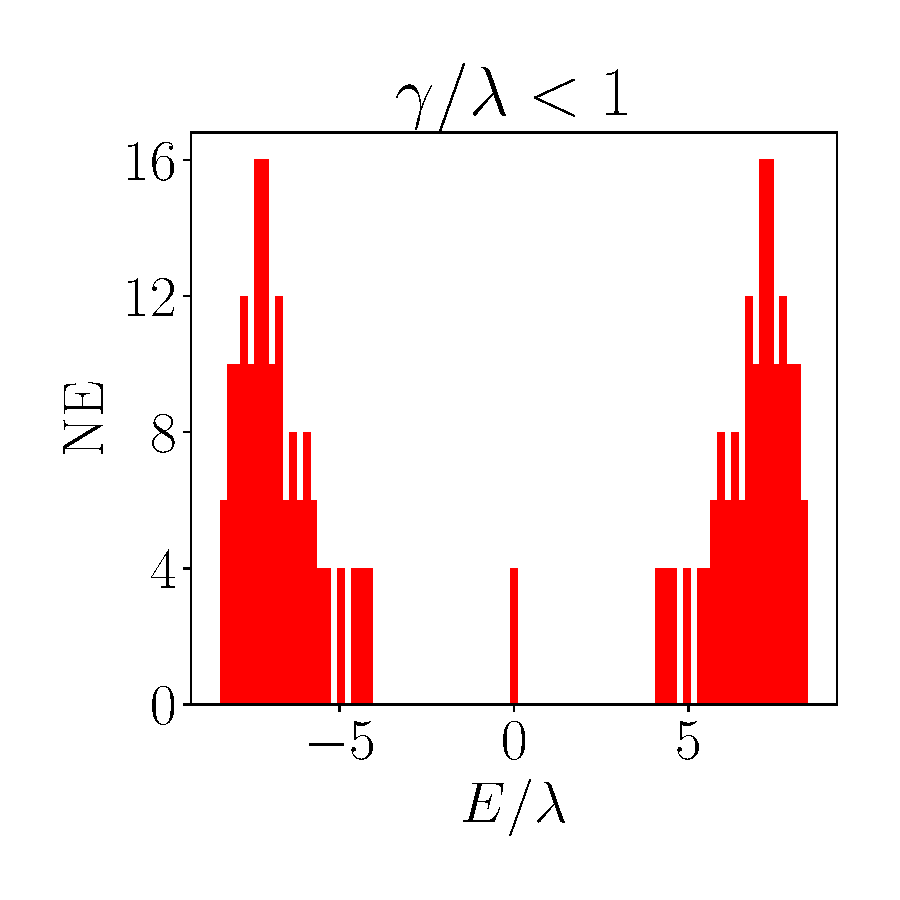
\includegraphics[width=\textwidth]{Imagenes/Resultados_Hoti_Cuadrado/bars_square1.pdf}
     \end{subfigure}\hspace*{1em}
     \begin{subfigure}[b!]{0.3 \textwidth}
         \caption{}
         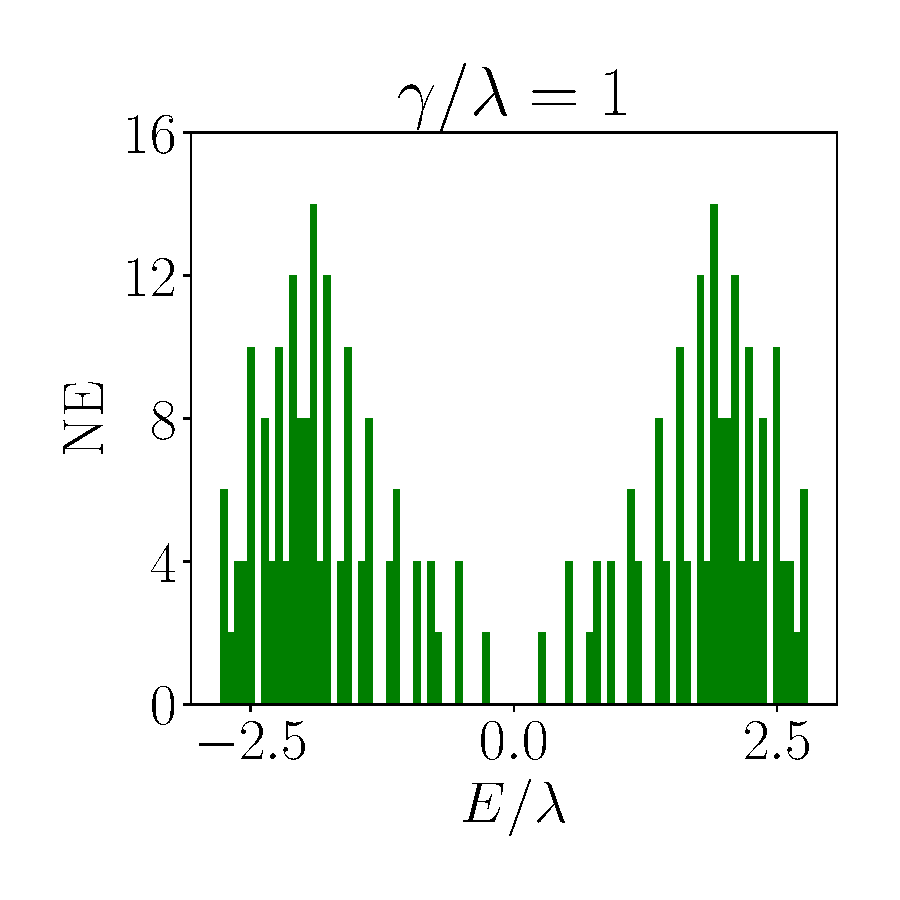
\includegraphics[width=\textwidth]{Imagenes/Resultados_Hoti_Cuadrado/bars_square2.pdf}
     \end{subfigure}\hspace*{1em}
     \begin{subfigure}[b!]{0.3 \textwidth}
         \caption{}
         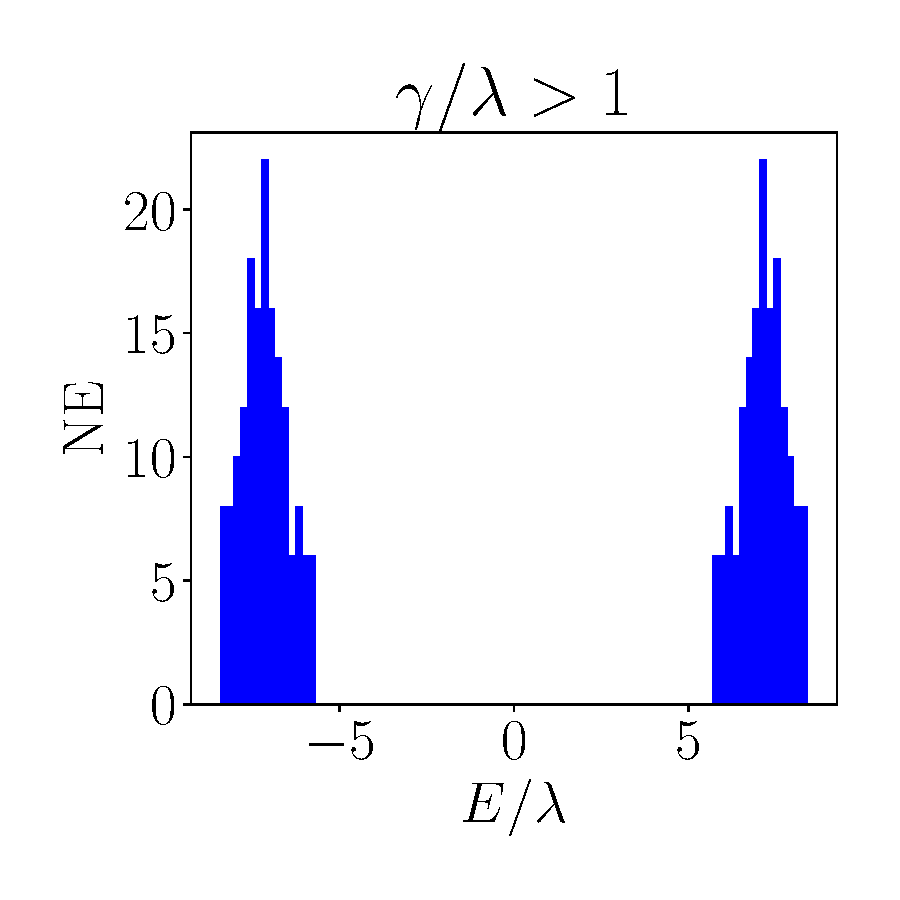
\includegraphics[width=\textwidth]{Imagenes/Resultados_Hoti_Cuadrado/bars_square3.pdf}
     \end{subfigure}\hspace*{1em}\vspace*{-0.5em}
        \caption{Numero de estados por energía en un red con geometría cuadrada para diferentes valores de los parámetros de salto, \textbf{a)} $\gamma /\lambda = 1/2$, \textbf{b)} $\gamma /\lambda = 1$, \textbf{c)} $\gamma /\lambda = 2$.}
        \label{fig:Dos_Cuadrado}
\end{figure}
En la figura \ref{fig:Dos_Cuadrado} podemos ver el comportamiento del número de estados por energía para diferentes valores de $\gamma/\lambda$ y para el modelo de BBH para una red cristalina cuadrada [sec.\ref{sec:Modelo_BBH_square_and_Fractal}]. Notemos que para los valores de $\gamma/\lambda>1$ [Fig.\ref{fig:Dos_Cuadrado} \textbf{(c)}] podemos ver un claro gap energético, lo cual indicaría que nuestra red cristalina se encuentra en un estado trivial, es decir, es un aislante común. Para los valores de $\gamma/\lambda<1$ [Fig. \ref{fig:Dos_Cuadrado} \textbf{(a)}] aparecen 4 estados degenerados carentes de gap en la energía de Fermi, estos aparecen como consecuencia de la finitud de la red cristalina por lo que les llamaremos estados de borde, esta fase del la red es conocida como fase topológica. En la figura \ref{fig:Dos_Cuadrado} \textbf{(c)} para $\gamma/\lambda = 1$ vemos que el gap energético de la red cristalina se cierra, lo cual indica la posible transición de fase entre el estado topológico y trivial con la variación de los parámetros de salto $\gamma/\lambda$ de la red cristalina.


\begin{figure}[h!]
     \centering
    \captionsetup[sub]{font=small}
     \begin{subfigure}[b!]{0.44 \textwidth}
         \caption{}
         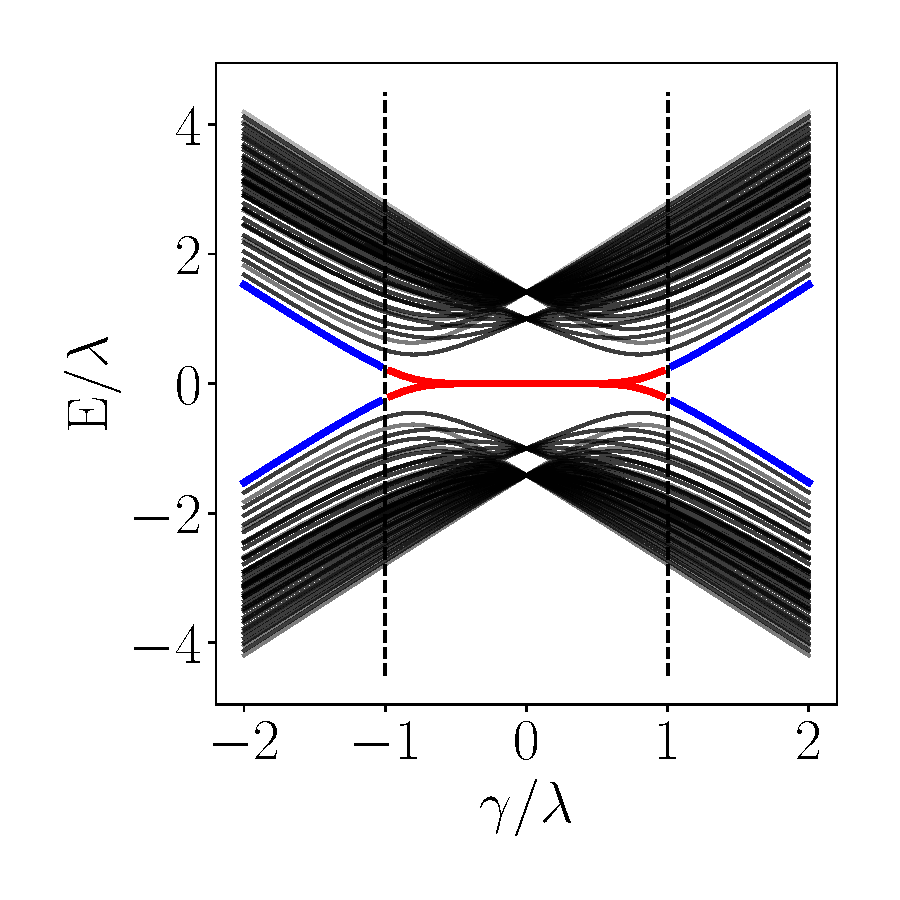
\includegraphics[width=\textwidth]{Imagenes/Resultados_Hoti_Cuadrado/bands_square_shh.pdf}
         \label{}
     \end{subfigure}\hspace*{1em}
     \begin{subfigure}[b!]{0.56 \textwidth}
         \caption{}
         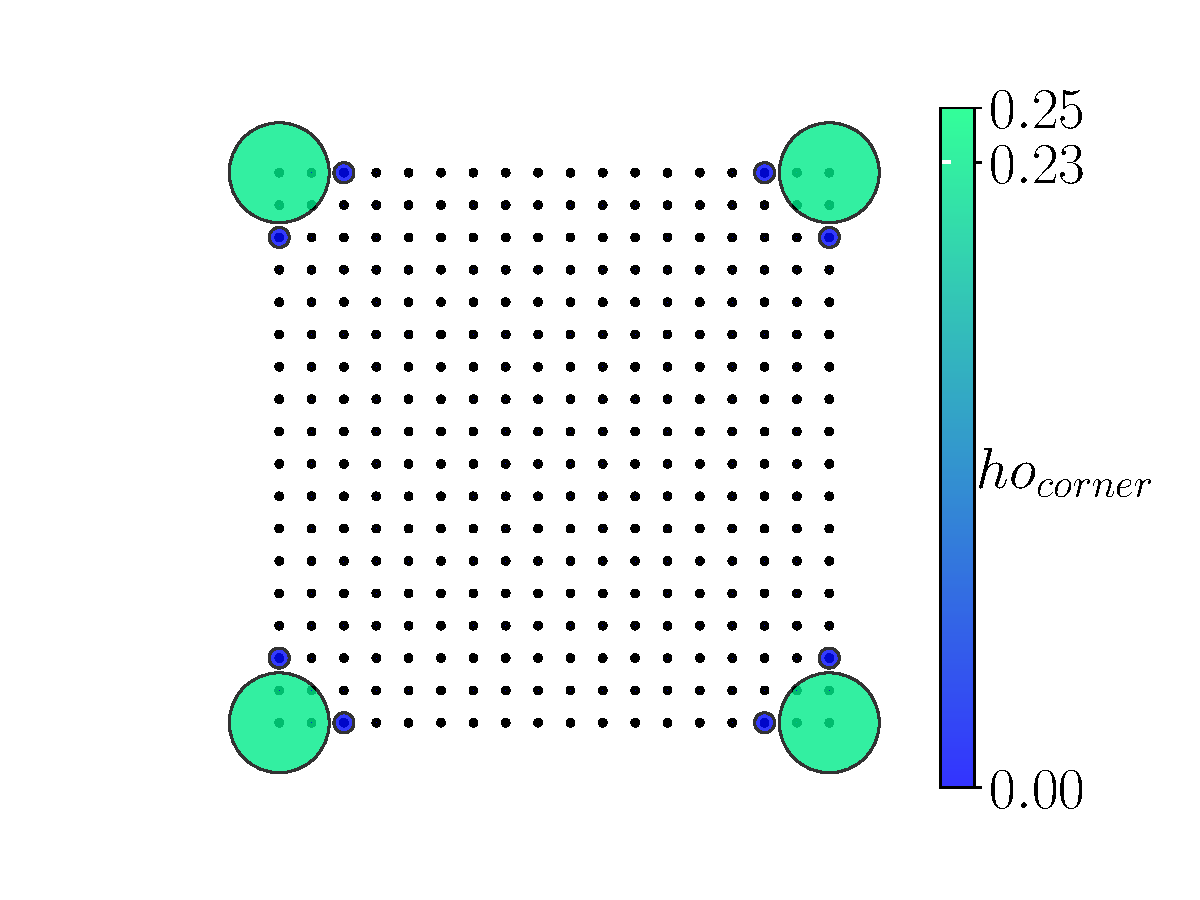
\includegraphics[width=\textwidth]{Imagenes/Resultados_Hoti_Cuadrado/proyection_square.pdf}
         \label{}
     \end{subfigure}\hspace*{1em} \vspace*{-1.5em}
        \caption{\textbf{a)}Espectro de energía del sistema con geometría cuadrada y condiciones abiertas a la frontera, como función de $\gamma/\lambda$. Las energías centrales coloreadas en rojo corresponde a los 4 estados localizados en las esquinas. \textbf{b)} Densidad de probabilidad en un fase no trivial donde $\gamma = 1,\, \, \lambda = 4.5$, en un red cuadrada de $18\times18$ sitios.}
    \label{fig:Pram_Proy_cuadrado}
\end{figure}


\begin{figure}[h!]
    \centering
   \captionsetup[sub]{font=small}

    \begin{subfigure}[b!]{0.5 \textwidth}
        \caption{}
        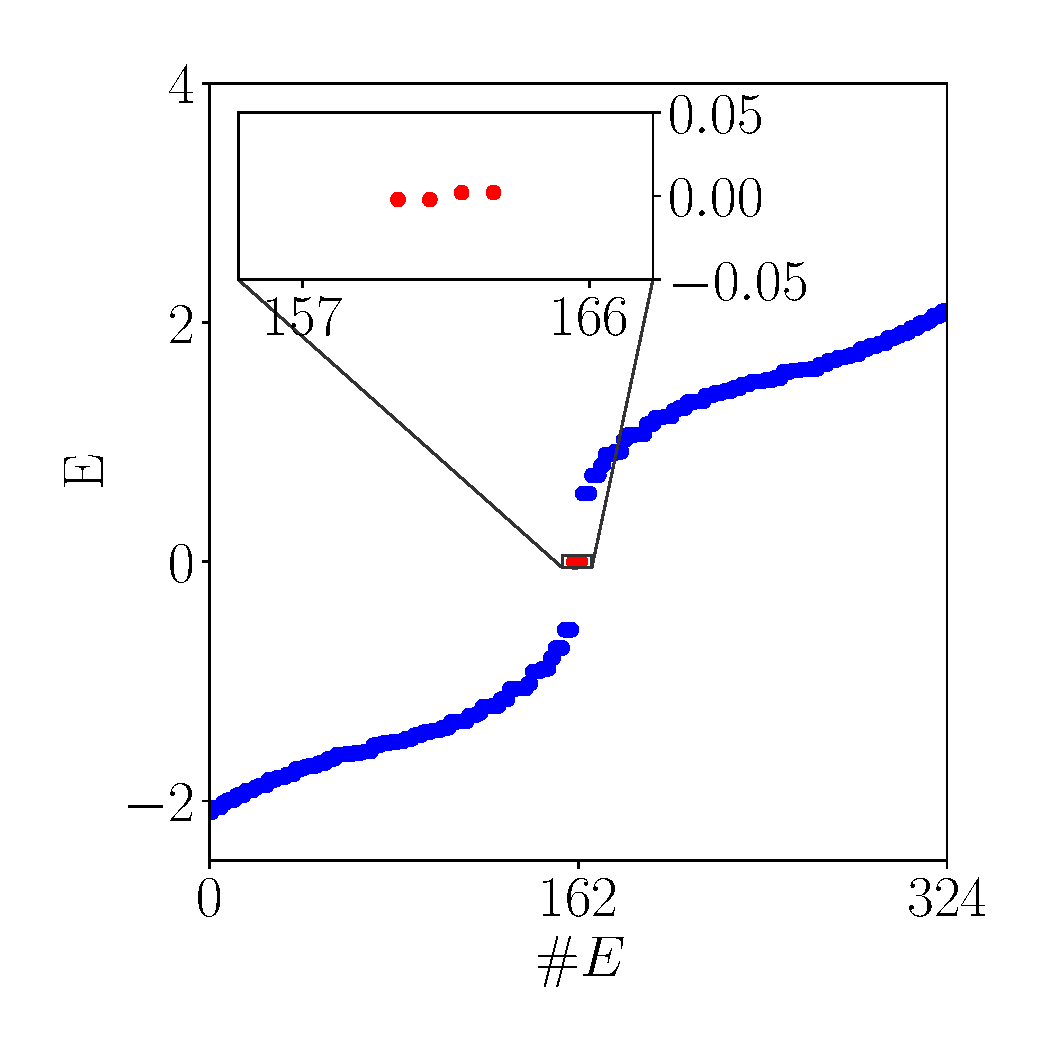
\includegraphics[width=\textwidth]{Imagenes/Resultados_Hoti_Cuadrado/spectre_square.pdf}
    \end{subfigure}
    \begin{subfigure}[b!]{0.5 \textwidth}
        \caption{}
        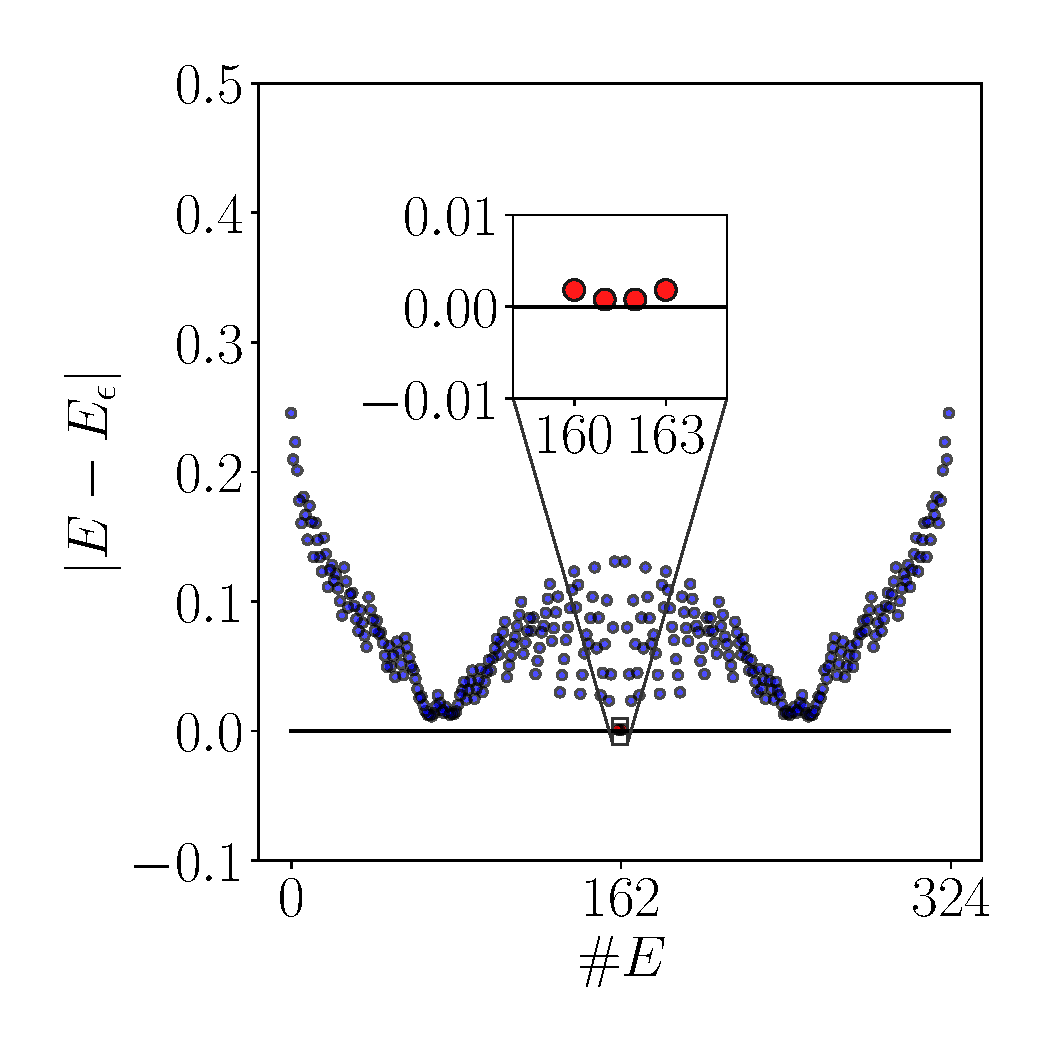
\includegraphics[width=\textwidth]{Imagenes/Resultados_Hoti_Cuadrado/spectre_square_epsi.pdf}
    \end{subfigure}\hspace*{-0.9em}
       \caption{\textbf{(a)} Espectro de energias odenadas para la red cristalina cuadrada con $\gamma = 0.5$ y $\lambda = 1.0$. \textbf{(b)} Cambio del espectro de energias cuando se perturban los parametros de salto con $\epsilon = 50\%$.}
       \label{fig:spectre_square_epsi}
\end{figure}


Para ver más a detalle como sucede esta transición de fase podemos hacer un seguimiento del espectro de energías conforme se varían los parámetros de salto y enfocarnos en las energías centrales correspondientes a los estados de borde [Fig.\ref{fig:Pram_Proy_cuadrado} \textbf{(a)}]. Las energías de los estados de borde están coloreadas con azul en la zona trivial y rojo en la zona topológica, en la zona $|\gamma/\lambda|>1$ el comportamiento de estas energías es similar a las energías de los estados del bulto de la red cristalna, sin embargo, en la zona $|\gamma/\lambda|>1$ las energías centrales se separan del bulto y se degeneran en la energía de Fermi. Al proyectar las densidades de probabilidad de los estados correspondientes a estas 4 energías podemos observar como se distibuyen estas densidades por la red, en la figura \ref{fig:Pram_Proy_cuadrado} \textbf{(b)} podemos ver que las densidades se encuentran claramente localizadas en las equinas de la red con probabilidad de aproximadamente $1/4$, lo cual definiria a nuestra red cirstalina como un aislante topológico de orden superior (HOTI \footnote{Siglas en ingles de High Order Topological Insulator}), donde el valor máximo de $\rho_{corner} = 1/4$ se alcanza en el caso limite $|\gamma/\lambda| = 0$ donde las celdas estarían totalmente cuatrimerizadas.


\vspace{1cm}
    \begin{figure}[thb!]
        \centering
        \begin{minipage}{0.8\textwidth}
           \captionsetup[sub]{font=small}
            \begin{minipage}[h!]{0.8\textwidth}
                \begin{subfigure}[b!]{0.44 \textwidth}
                    \caption{$\epsilon = 1\%$}
                    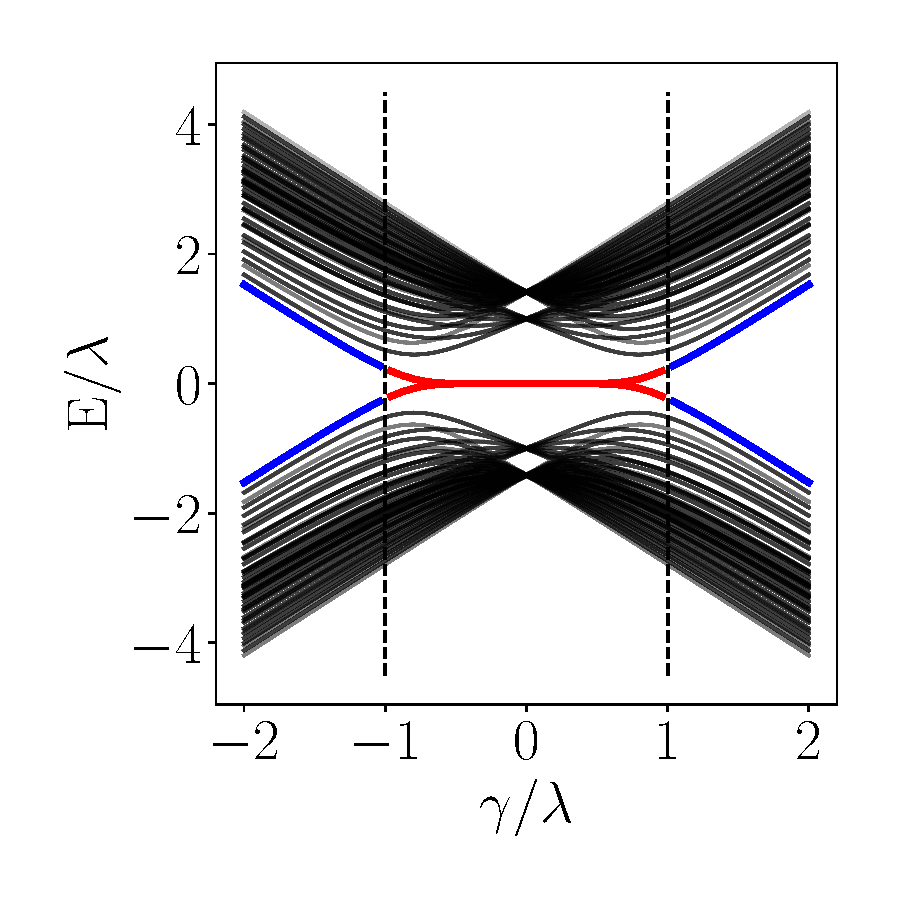
\includegraphics[width=\textwidth]{Imagenes/Resultados_Hoti_Cuadrado/bands_square_shh_0.01.pdf}
                \end{subfigure}\hspace*{-0.5em}
                \begin{subfigure}[b!]{0.56 \textwidth}
                    \caption*{}
                    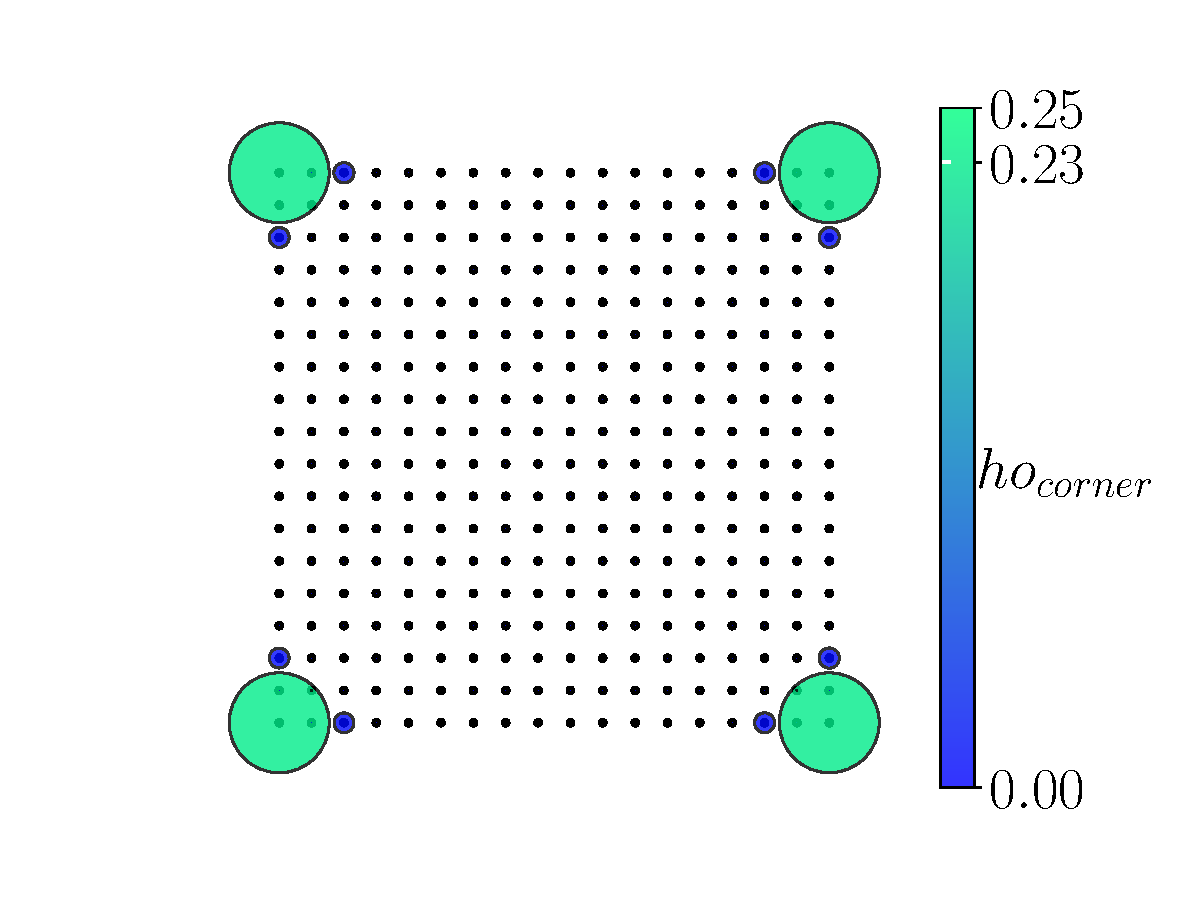
\includegraphics[width=\textwidth]{Imagenes/Resultados_Hoti_Cuadrado/proyection_square_0.01.pdf}
                \end{subfigure}\hspace*{-0.5em}
            \end{minipage}\vspace*{-1.5em}
            
            \begin{minipage}[h!]{0.8\textwidth}
                \begin{subfigure}[b!]{0.44 \textwidth}
                    \caption{$\epsilon = 5\%$}
                    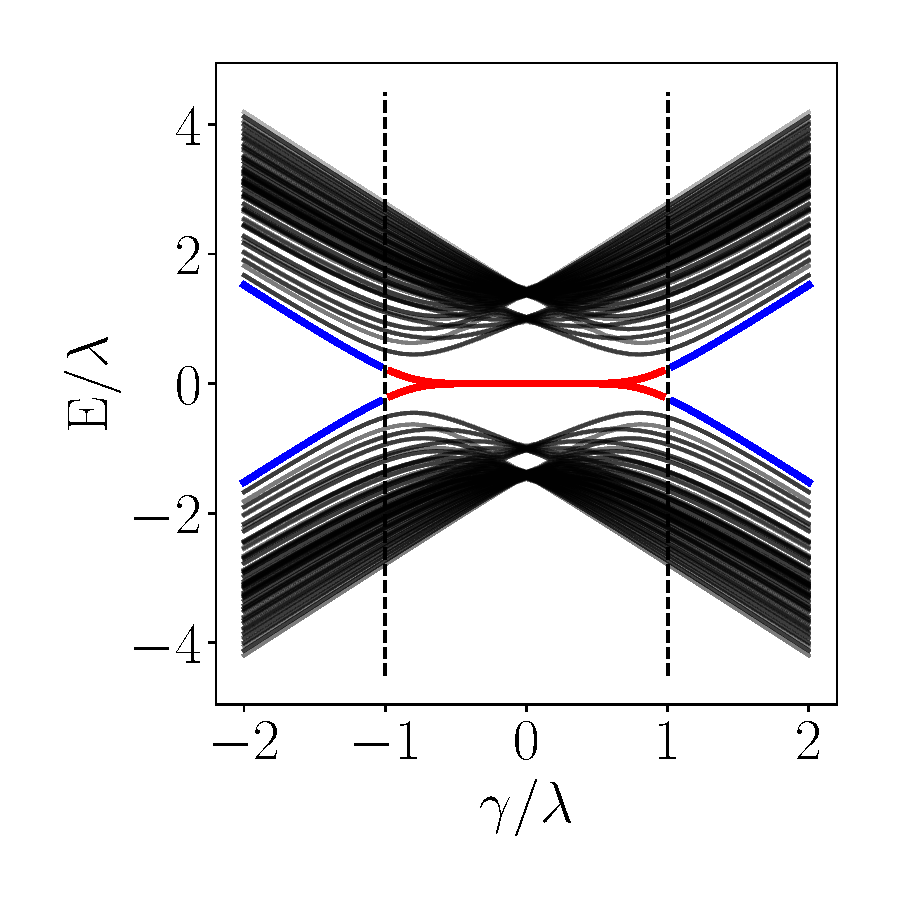
\includegraphics[width=\textwidth]{Imagenes/Resultados_Hoti_Cuadrado/bands_square_shh_0.05.pdf}
                \end{subfigure}\hspace*{-0.5em}
                \begin{subfigure}[b!]{0.56 \textwidth}
                    \caption*{}
                    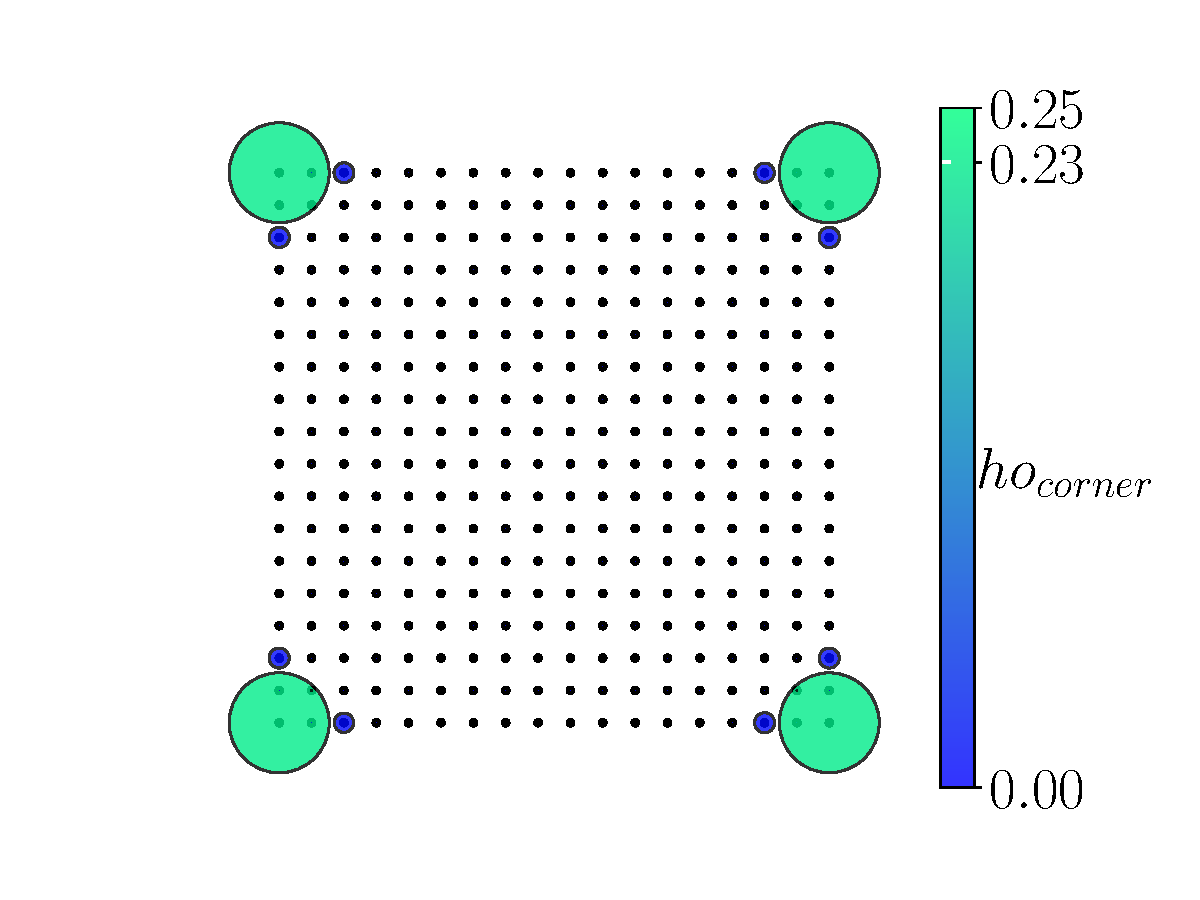
\includegraphics[width=\textwidth]{Imagenes/Resultados_Hoti_Cuadrado/proyection_square_0.05.pdf}
                \end{subfigure}\hspace*{-0.5em}
            \end{minipage}\vspace*{-1.5em}
            
            \begin{minipage}[h!]{0.8\textwidth}
                \begin{subfigure}[b!]{0.44 \textwidth}
                    \caption{$\epsilon = 10\%$}
                    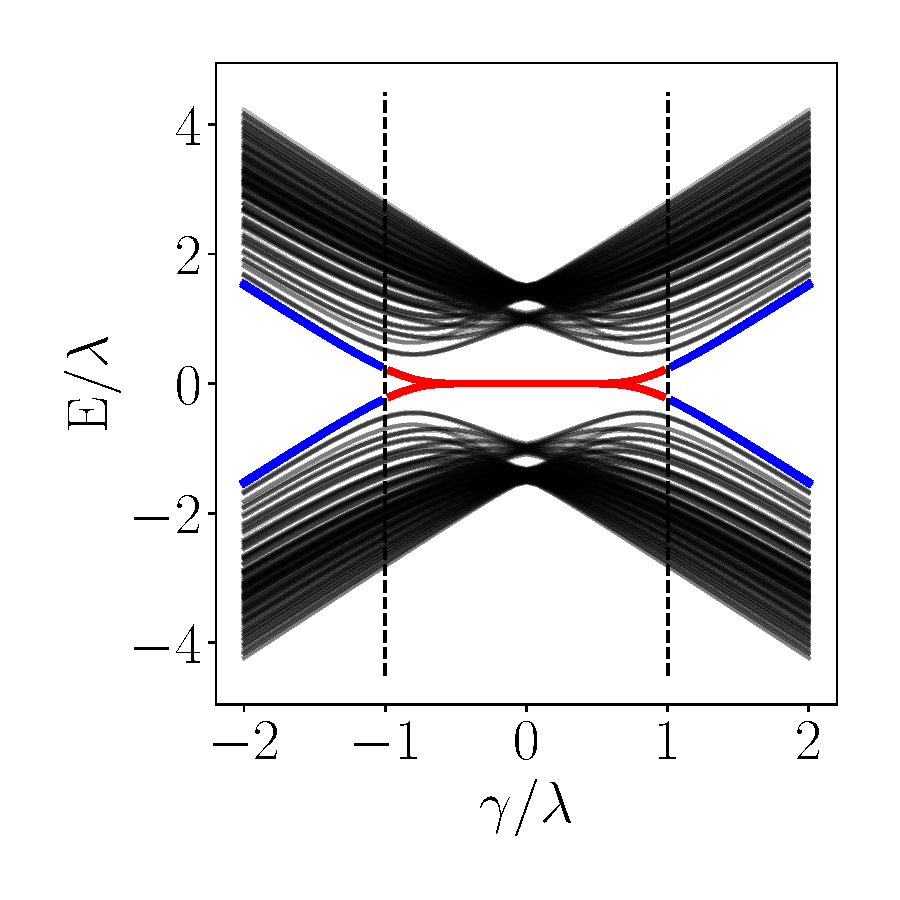
\includegraphics[width=\textwidth]{Imagenes/Resultados_Hoti_Cuadrado/bands_square_shh_0.1.pdf}
                \end{subfigure}\hspace*{-0.5em}
                \begin{subfigure}[b!]{0.56 \textwidth}
                    \caption*{}
                    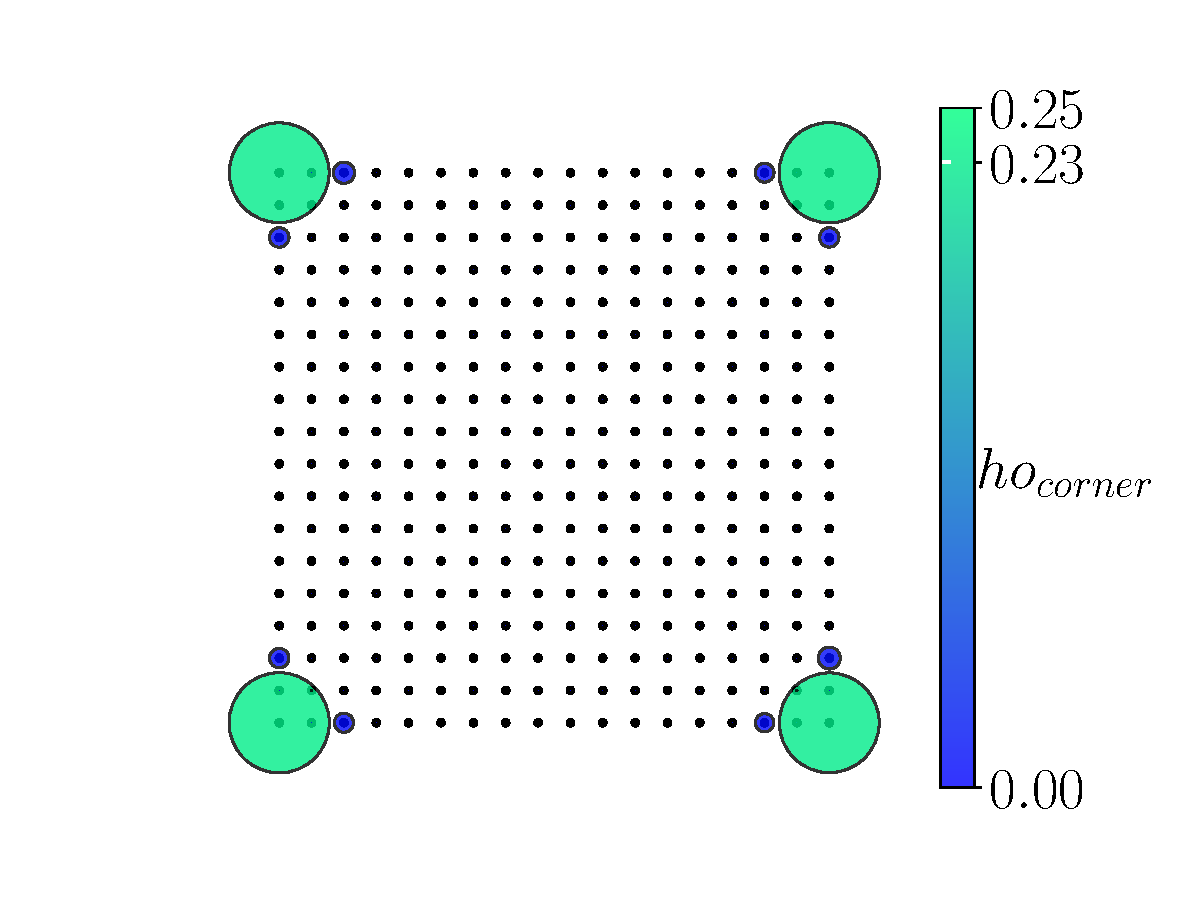
\includegraphics[width=\textwidth]{Imagenes/Resultados_Hoti_Cuadrado/proyection_square_0.1.pdf}
                \end{subfigure}\hspace*{-0.5em}
            \end{minipage}\vspace*{-1.5em}
            
            \begin{minipage}[h!]{0.8\textwidth}
                \begin{subfigure}[b!]{0.44 \textwidth}
                    \caption{$\epsilon = 30\%$}
                    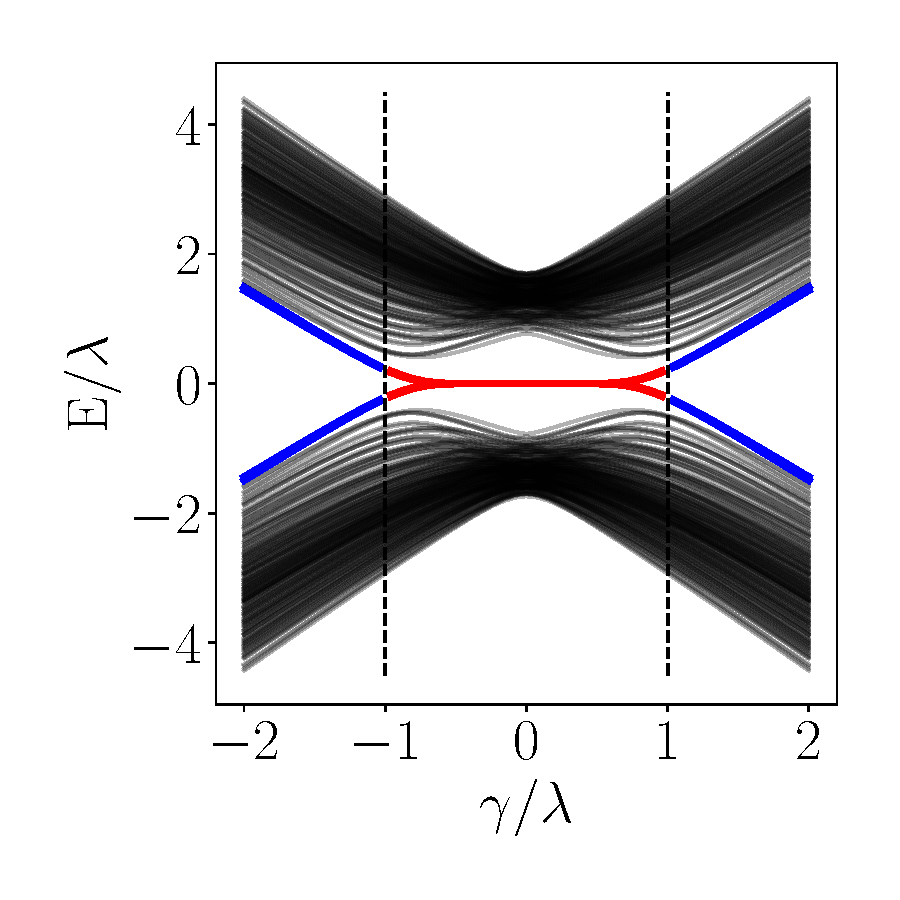
\includegraphics[width=\textwidth]{Imagenes/Resultados_Hoti_Cuadrado/bands_square_shh_0.3.pdf}
                \end{subfigure}\hspace*{-0.5em}
                \begin{subfigure}[b!]{0.56 \textwidth}
                    \caption*{}
                    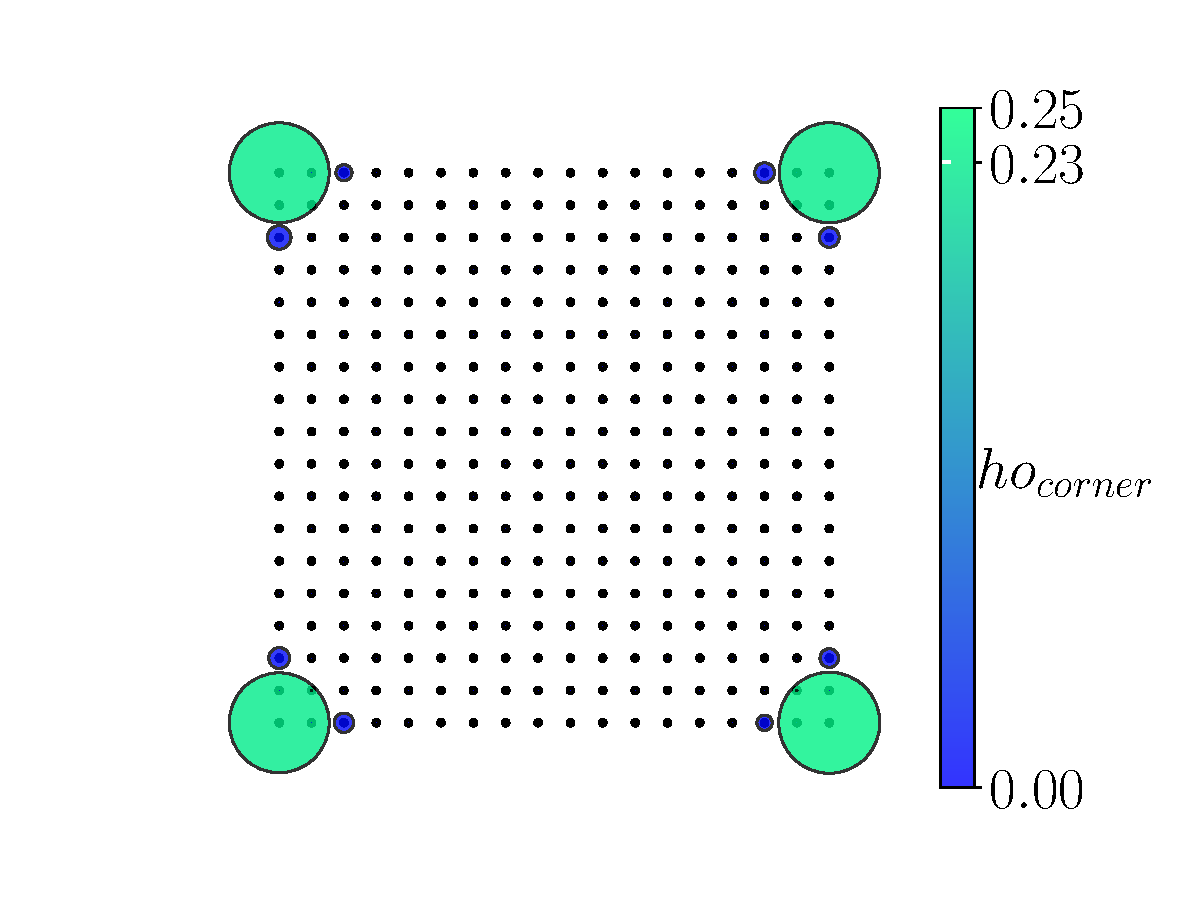
\includegraphics[width=\textwidth]{Imagenes/Resultados_Hoti_Cuadrado/proyection_square_0.3.pdf}
                \end{subfigure}\hspace*{-0.5em}
            \end{minipage}\vspace*{-1.5em}
            
            \begin{minipage}[h!]{0.8\textwidth}
                \begin{subfigure}[b!]{0.44 \textwidth}
                    \caption{$\epsilon = 50\%$}
                    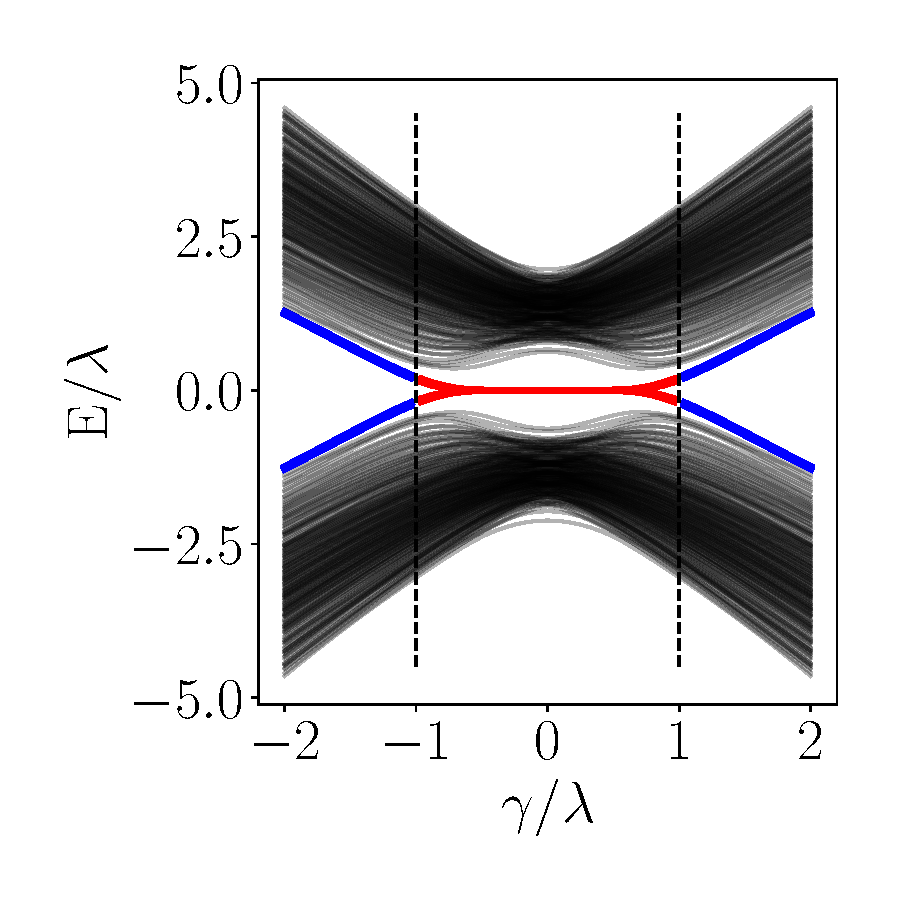
\includegraphics[width=\textwidth]{Imagenes/Resultados_Hoti_Cuadrado/bands_square_shh_0.5.pdf}
                \end{subfigure}\hspace*{-0.5em}
                \begin{subfigure}[b!]{0.56 \textwidth}
                    \caption*{}
                    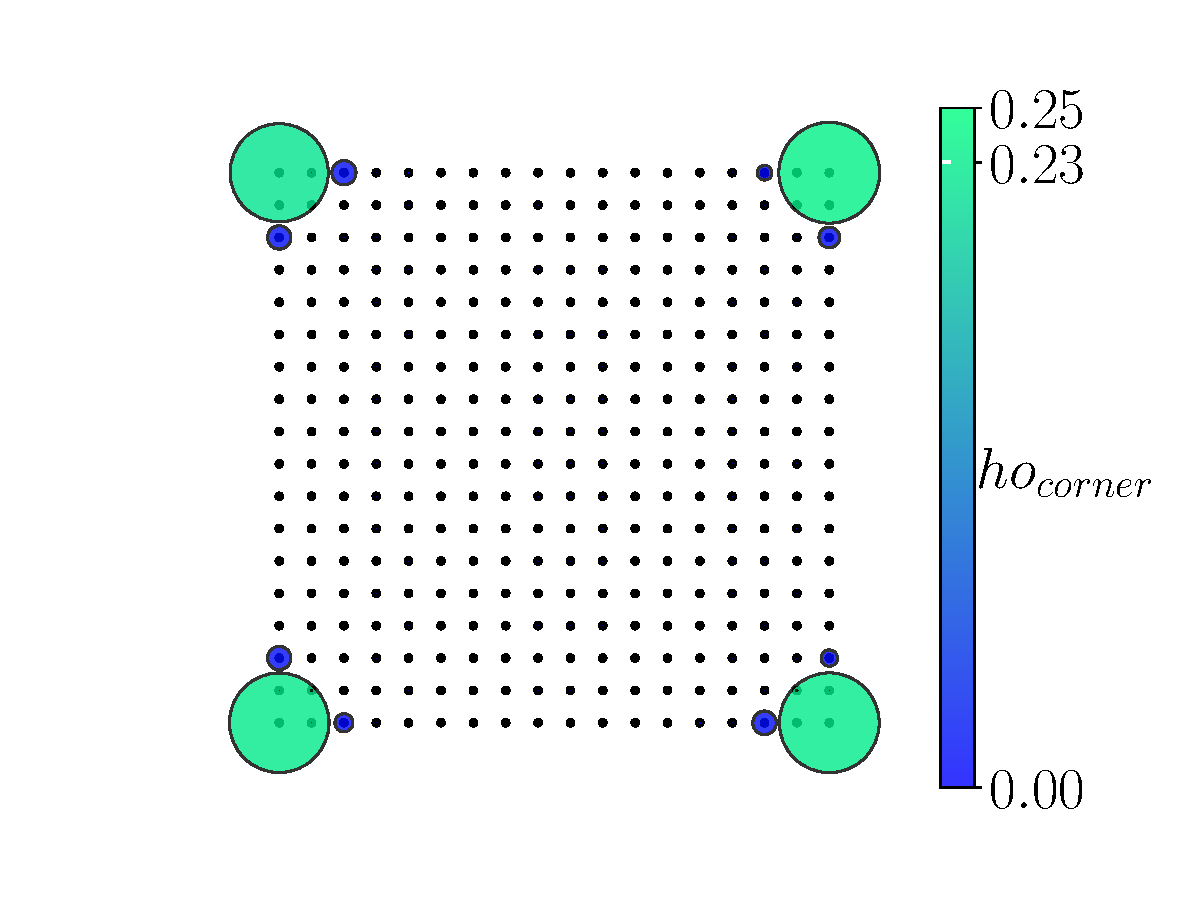
\includegraphics[width=\textwidth]{Imagenes/Resultados_Hoti_Cuadrado/proyection_square_0.5.pdf}
                \end{subfigure}\hspace*{-0.5em}
            \end{minipage}\vspace*{-0.5em}
        \end{minipage} 
           \caption{\textbf{(a)-(e)}En la columna derecha se muestra el espectro de energías en una red cuadrada como función de $\gamma/\lambda $ con un desorden aleatorio en los parámetros de salto, de tamaño $\delta$. Las lineas rojas corresponden a los cuatro estados degenerados que representan los estados localizados en las esquinas. En la columna izquierda se muestra la densidad de probabilidad de la fase no trivial donde $\gamma' = \gamma( 1 \pm \epsilon) ,\, \, \lambda' = \lambda( 1 \pm \epsilon)$.  }
           \label{fig:Pram_Proy_Delta_cuadrado}
         
       \end{figure} 

    



También estos estados son robustos ante perturbaciones adiabáticas como se puede observar en las figuras \ref{fig:para_proy_Delta_fractal} \textbf{(a)-(e)} donde las perturbaciones se ejercieron sobre los parámetros de salto $\gamma' = \gamma( 1 \pm \epsilon) ,\, \, \lambda' = \lambda( 1 \pm \epsilon)$ con $\epsilon = [1\%, 5\%, 10\%,30\%,50\%,]$, se puede notar que estas variaciones solo cambian las energías correspondientes a los estados del bulto [Fig.\ref{fig:spectre_square_epsi} \textbf{(b)}], mientras los estados de borde que permanecen robustos con $|E - E_{\epsilon = 50\%}| < 10^{-3}$. Esta robustes se ve reflejada en que los estados de borde que se localizan en las esquinas permanecen imperturbables.


\section{Hoti Fractal}

\begin{figure}[h!]
     \centering
    \captionsetup[sub]{font=small}
     \begin{subfigure}[b!]{0.3 \textwidth}
         \caption{}
         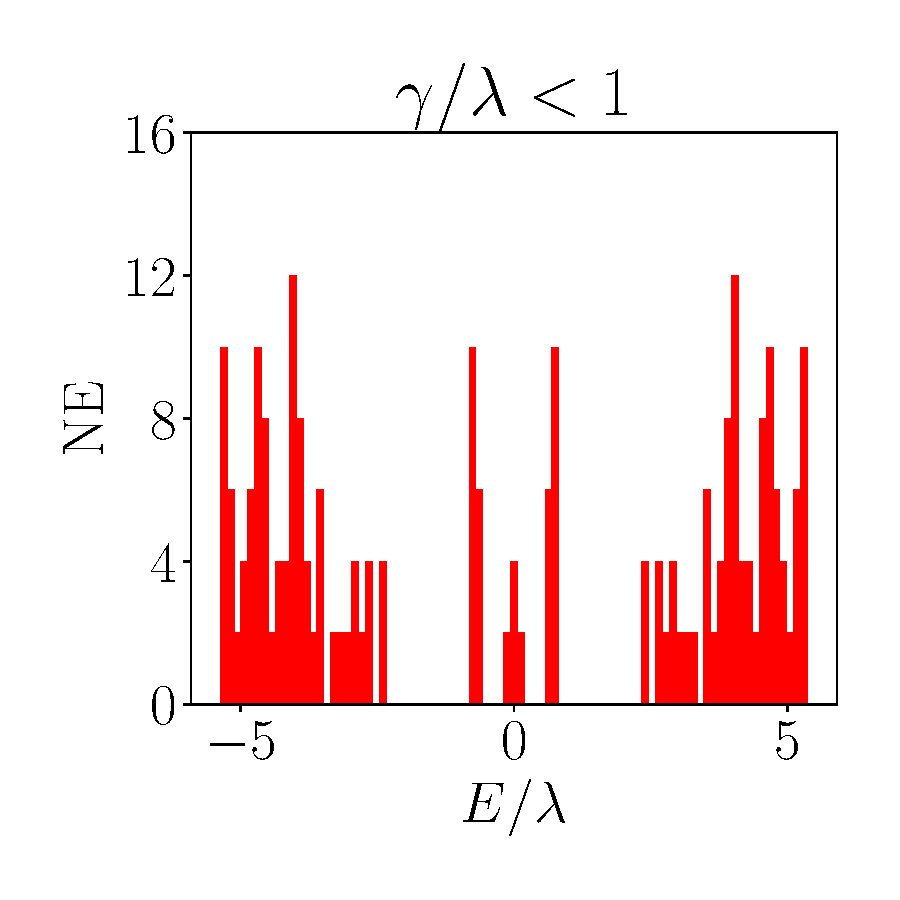
\includegraphics[width=\textwidth]{Imagenes/Resultados_Hoti_Fractal/bars_square1.pdf}
         \label{}
     \end{subfigure}\hspace*{1em}
     \begin{subfigure}[b!]{0.3 \textwidth}
         \caption{}
         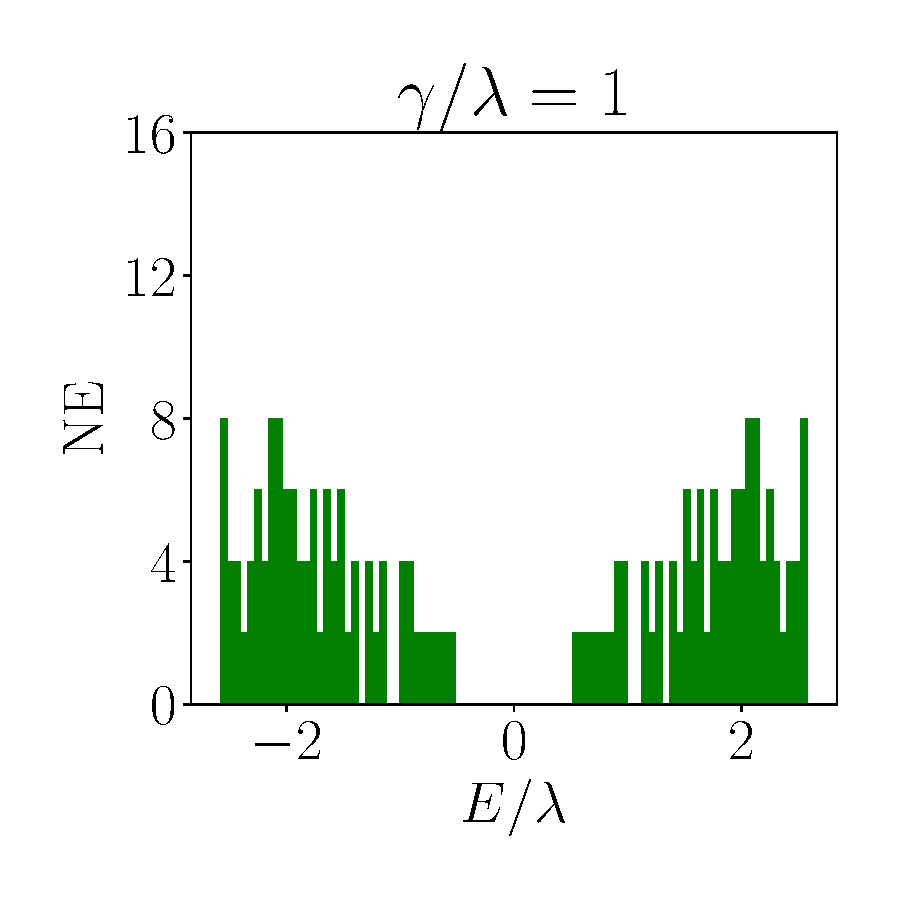
\includegraphics[width=\textwidth]{Imagenes/Resultados_Hoti_Fractal/bars_square2.pdf}
         \label{}
     \end{subfigure}\hspace*{1em}
     \begin{subfigure}[b!]{0.3 \textwidth}
         \caption{}
         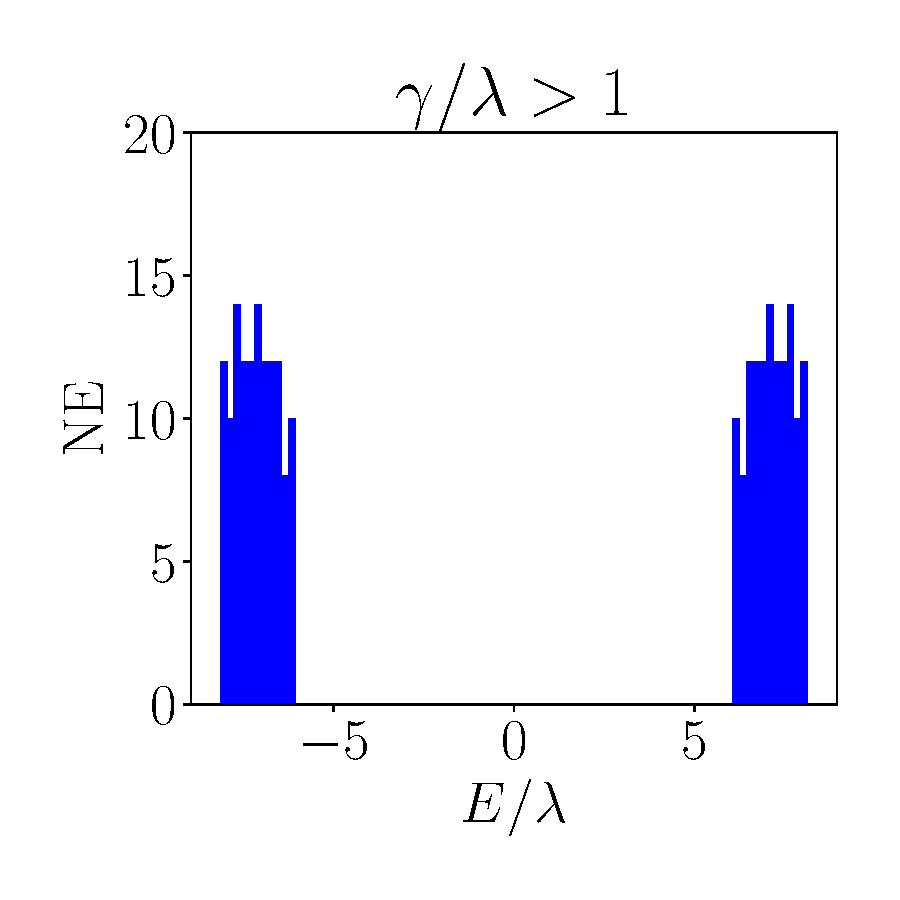
\includegraphics[width=\textwidth]{Imagenes/Resultados_Hoti_Fractal/bars_square3.pdf}
         \label{}
     \end{subfigure}\hspace*{1em}\vspace*{-1.5em}
        \caption{Cantidad de estados por energía en un red con geometría Fractal (2da generación) para diferentes valores de los parámetros de salto, \textbf{a)} $\gamma /\lambda = 1/2$, \textbf{b)} $\gamma /\lambda = 1$, \textbf{c)} $\gamma /\lambda = 2$.}
    \label{fig:Dos_fractal}
\end{figure}


En la figura \ref{fig:Dos_fractal} observamos el número de estados por energía para el modelo de la red de Sierpinski para distintos valores de los parámetros de salto $\gamma/\lambda$. Para valores de $\gamma/\lambda < 1$ seguimos teniendo una la diferencición de los estados de borde y de bulto al igual que 4 estados centrales, sin embargo, a diferencia de el caso de la red cuadrada, estos estados se degeneran sobre la energia de Fermi para valores mas cercanos a esta  $\gamma/\lambda < 0.5$, estos estados aparecen acompañados por otras energias tambien cercanas a la energía de Fermi, estas corresponden a los nuevos estados de borde consecuentes con la geometría de la red de Sierpinski. También podemos ver que para valores $\gamma/\lambda > 1$, al igual que en la red cuadrada, tenemos un histograma correspondiente a una fase trivial, en medio de esta transición tenemos $\gamma/\lambda = 1$ donde se puede ver como la brecha de las energías comienzan a cerrarce, esto se puede ver más a detalle en las figura \ref{fig:Param_Proy_fractal} \textbf{(a)}, donde se puede apreciar el cambio del espectro de las energías conforme se varían los parámetros de salto, en esta figura podemos notar como a partir de estos valores de $\gamma/\lambda = 1$ se comienza a diferenciar el comportamiento de borde del comportamiento de bulto. Notemos que las energías correspondiente a los estados de borde se comienzan a cerrar hasta degenerarse todas en la energía de fermi cuando $\gamma/\lambda = 0$ [Fig. \ref{fig:Param_Proy_fractal} \textbf{(b)}], es decir, cuando las celdas están totalmente cuatrimerizadas, para evitar este caso es necesario que la elección de los 4 estados centrales correspondientes a la acumulación de la densidad de estados en las esquinas se sintonice en puntos de $\gamma/\lambda \in [0.5,0)$ [fig. \ref{fig:Param_Proy_fractal} \textbf{(c)}]. Conforme nos acerquemos al caso limite de $\gamma/\lambda = 0$ la densidad de de probabilidad acumulada en las esquinas también cumple que $\rho_{corner} \approx 1/4$.


\begin{figure}[h!]
     \centering
    \captionsetup[sub]{font=small}
     \begin{subfigure}[b!]{0.24 \textwidth}
         \caption{}
         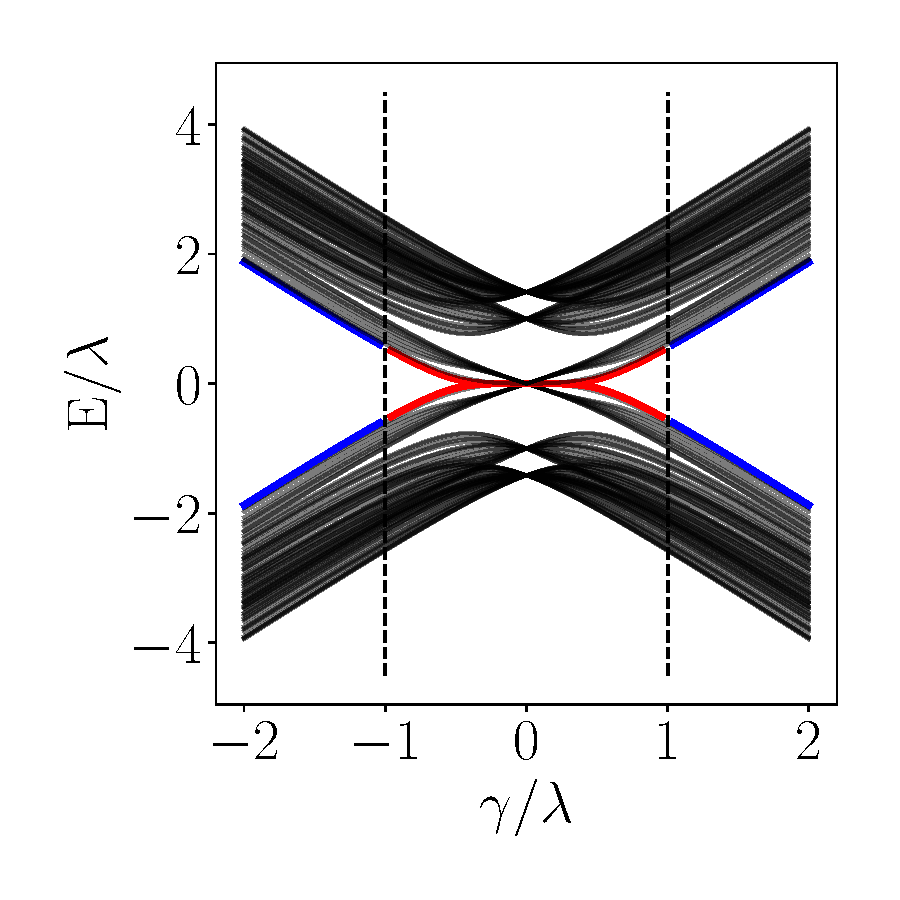
\includegraphics[width=\textwidth]{Imagenes/Resultados_Hoti_Fractal/bands_square_shh.pdf}
     \end{subfigure}\hspace*{-0.5em}
     \begin{subfigure}[b!]{0.24 \textwidth}
         \caption{}
         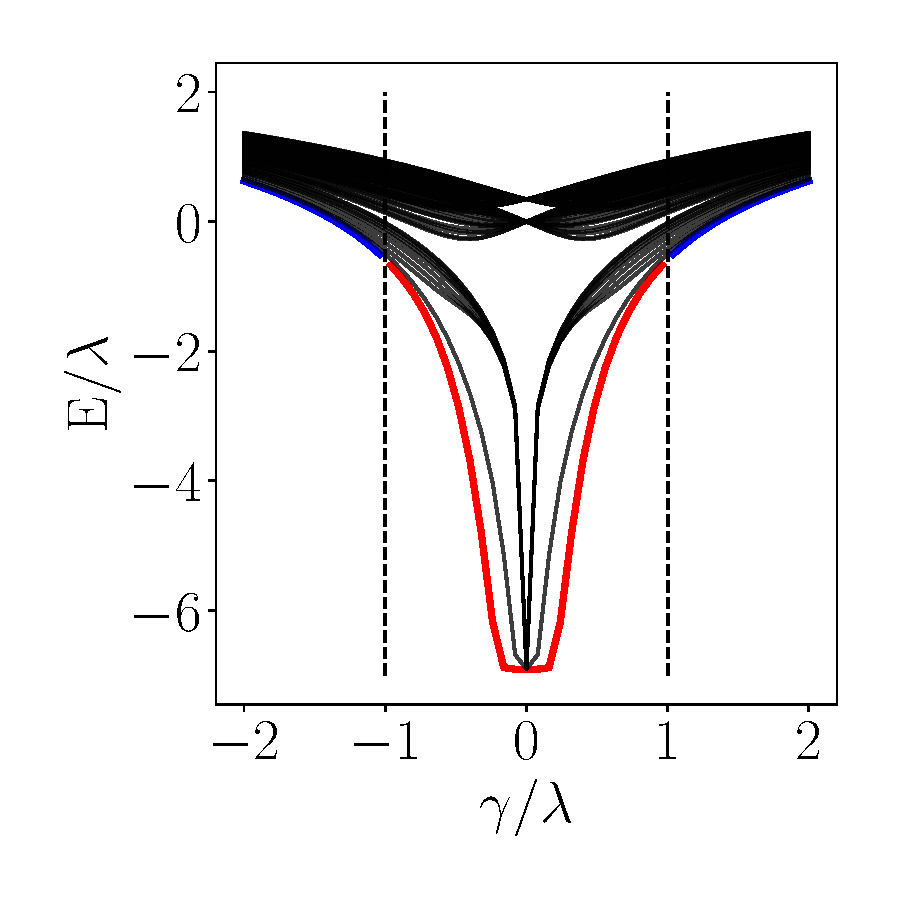
\includegraphics[width=\textwidth]{Imagenes/Resultados_Hoti_Fractal/bands_square_shh_log.pdf}
     \end{subfigure}\hspace*{-0.5em} 
      \begin{subfigure}[b!]{0.28 \textwidth}
         \caption{}
         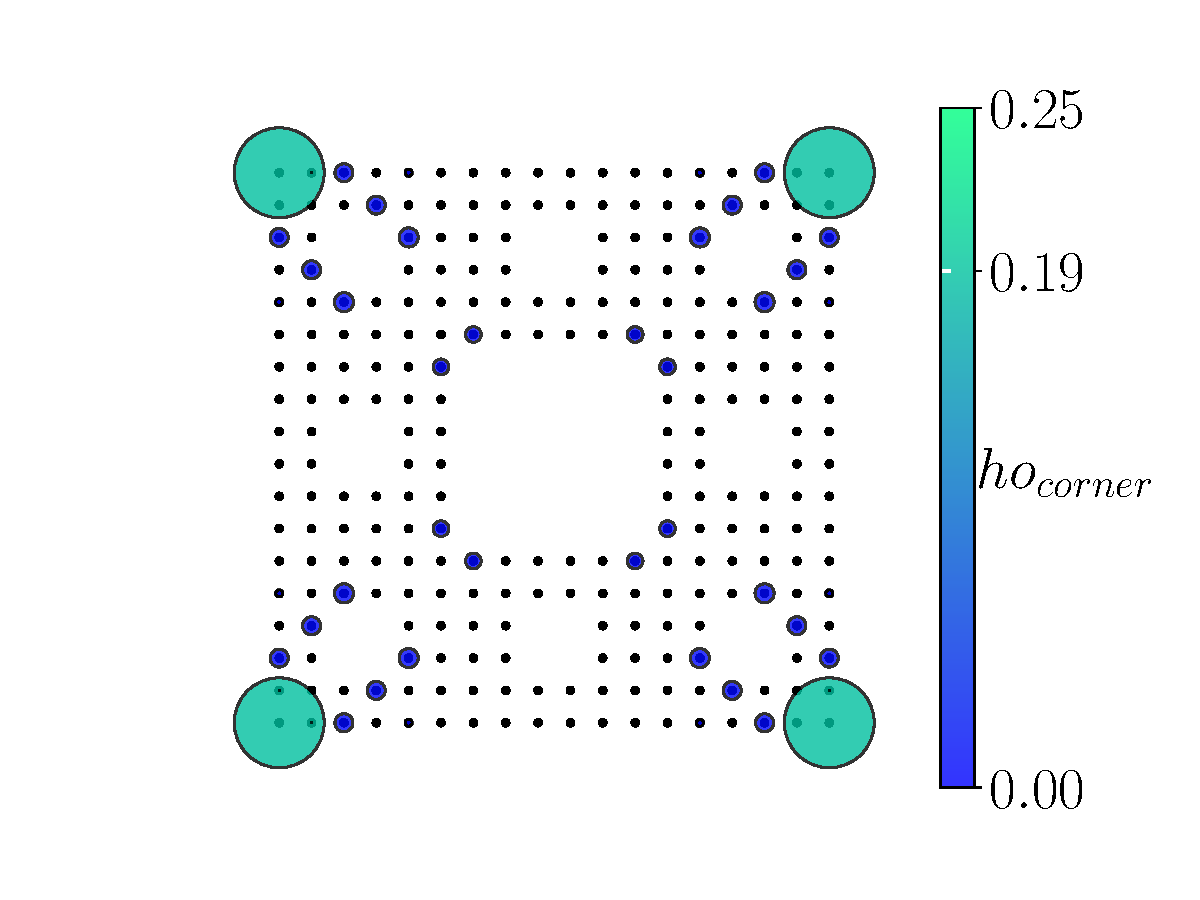
\includegraphics[width=\textwidth]{Imagenes/Resultados_Hoti_Fractal/proyection_square.pdf}
     \end{subfigure}\hspace*{-0.5em} 
     \begin{subfigure}[b!]{0.24 \textwidth}
        \caption{}
        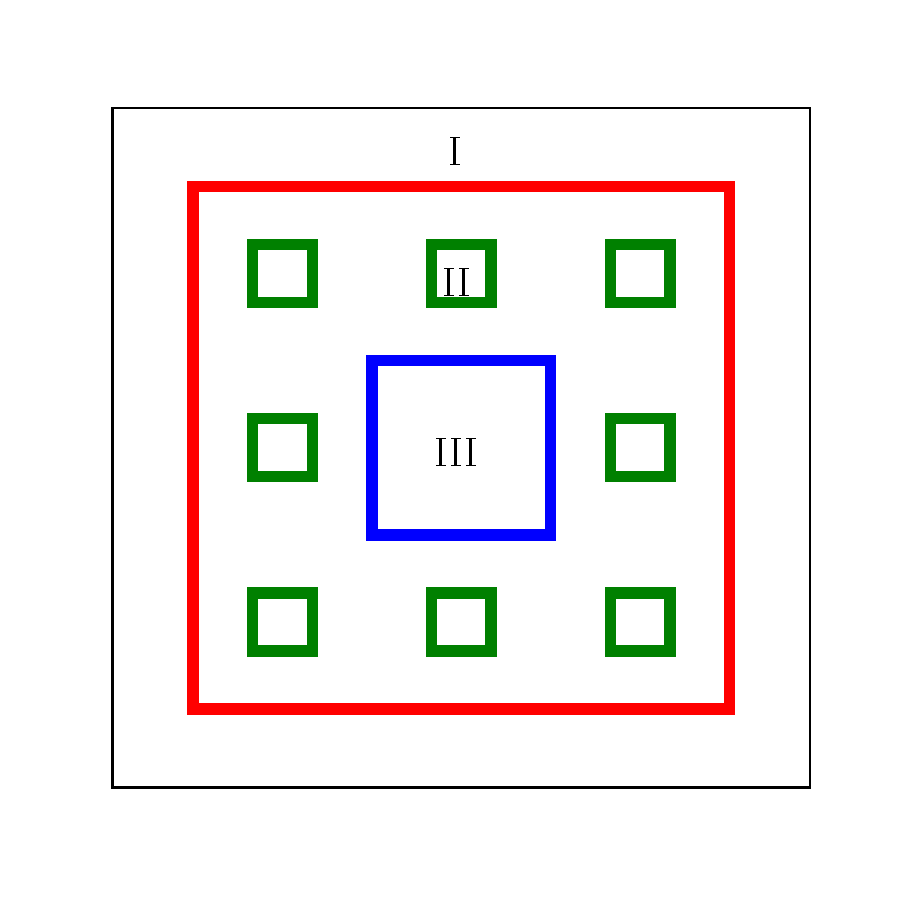
\includegraphics[width=\textwidth]{Imagenes/Models/sierpinski_carpet_color.pdf}
    \end{subfigure}\hspace*{-0.5em} \vspace*{-0.5em}
        \caption{\textbf{(a)} Espectro de energía del sistema con geometría fractal y condiciones abiertas a la frontera, como función de $\gamma/\lambda$. \textbf{(b)} Espectro de energía en escala logarítmica del sistema antes mencionado. Las lineas rojas corresponden a los cuatro estados degenerados que representan los estados localizados en las esquinas. \textbf{(c)} Densidad de probabilidad en un fase no trivial donde $\gamma = 1,\, \, \lambda = 4.5$, en un red fractal de 2da generación. \textbf{(d)} Bordes de la red Fractal de Sierpinski de 2da generación.}
\label{fig:Param_Proy_fractal}
\end{figure}

Si pensamos a la red de Sierpinski como una red cristalina cuadrada que fue sometida a transformaciones espaciales discontinuas como lo es abrirle agujeros, por el anlisis anterior, podemos decir que es posible reporducir las propiedades el Hoti cuadrado en el un HOTI fractal para ciertos parámetros de $\gamma/\lambda$, es decir, es posible conseguir que las densidades de estado se encuentren en localizadas en las esquinas aun con perturbaciones de perforación en la geometría, sin embargo notemos que la estructura de la celda unitaria sigue siendo la misma. Por lo tanto las propiedades topologicas de estas estructuras recide en las simetrias que pueda preservar o romper la celda. 
Estos estados también presentan robustes ante perturbaciones en los parámetros de salto, aunque en menor medida, como se puede ver en la figura \ref{fig:para_proy_Delta_fractal} \textbf{(a)-(e)} conforme $\epsilon$ crece las perturbaciones afectan primero a las energías del bulto y posteriormente deformando la trayectorias de las lineas correspondientes a las energías de borde II y III [Fig. \ref{fig:Param_Proy_fractal} \textbf{(d)}], sin embargo las energías de borde de la zona I,  que corresponden a los estados en las con probabilidades concentradas en las esquinas, no son modificados, sin embargo, al proyectar la densidades de probabilidad sobre la red cristalina podemos ver que las variaciones con $\epsilon \leq 30\%$ generan asimetrías en las las acumulaciones de densidades que se encuentran distribuidas en las fronteras internas de la red.

En la Figura \ref{fig:spectre_fractal_epsi} \textbf{(b)} podemos ver como las energías del bode I  se mantienen robustos con $|E - E_{\epsilon = 30\%}| < 10^{-3}$, es importante recalcar que las energias de borde III comienzan a robustecerse conforme crece el tamaño de generación del fractal, esto significaría que los estados de borde se vuelven Topologicos conforme el bodrde gana significacia respecto al tamaño de la red. Lamentablemente debido a las limitaciones computacionales, por el tamaño de las redes fractales, no fue posible estudiar a fondo esta caracteristica de la red fractal de Sierpinski para mayores generaciones.





\begin{figure}[tbh!]
     \centering
    \captionsetup[sub]{font=small}
     \begin{minipage}[h!]{0.9\textwidth}
         \begin{subfigure}[b!]{0.3 \textwidth}
            \caption{$\epsilon = 1\%$}             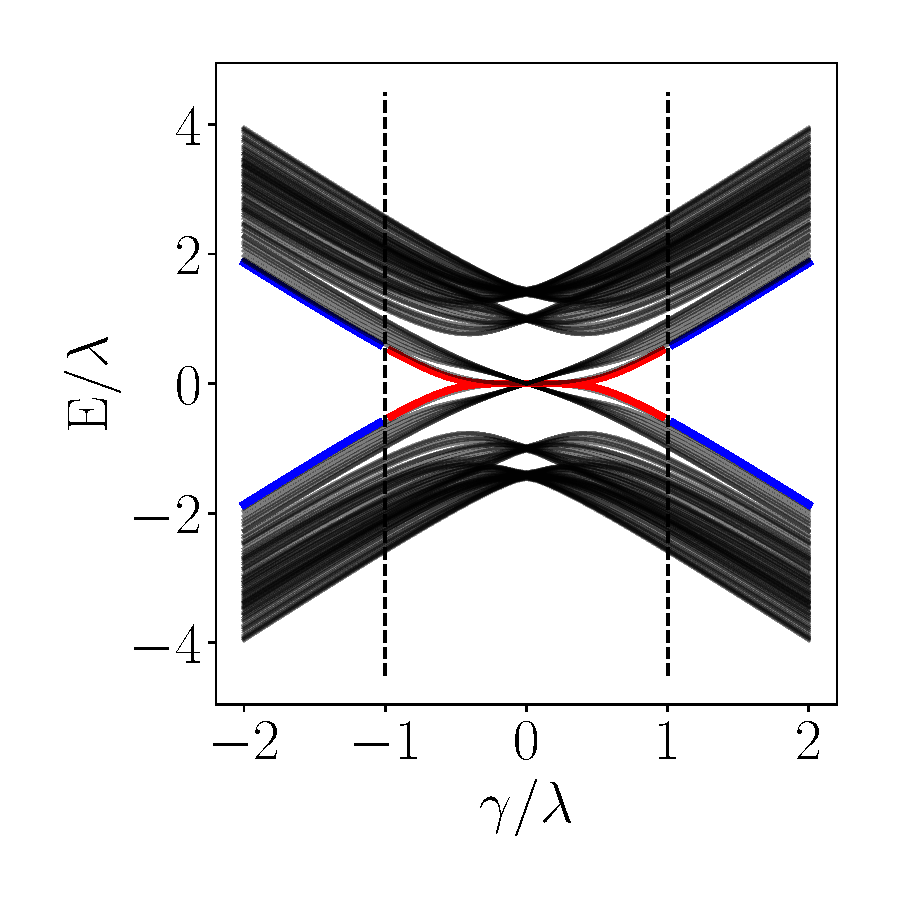
\includegraphics[width=\textwidth]{Imagenes/Resultados_Hoti_Fractal/bands_square_shh_0.05.pdf}
         \end{subfigure}\hspace*{-0.5em}
         \begin{subfigure}[b!]{0.3 \textwidth}
             \caption*{}
             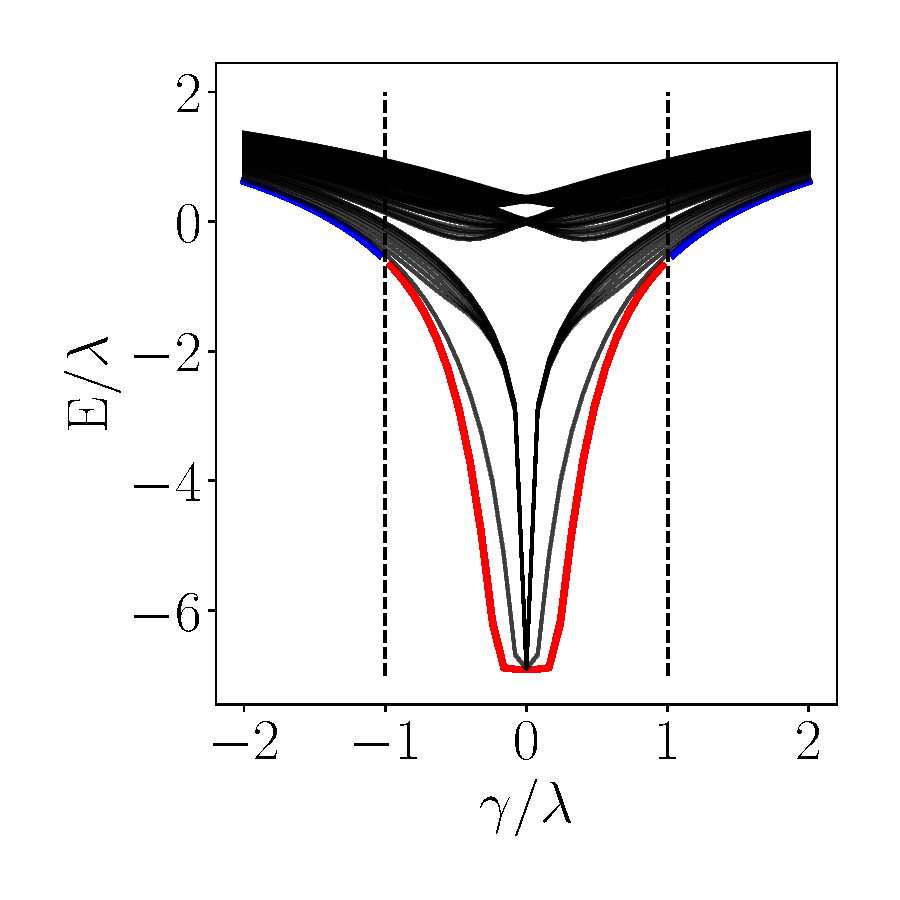
\includegraphics[width=\textwidth]{Imagenes/Resultados_Hoti_Fractal/bands_square_shh_log0.05.pdf}
         \end{subfigure}\hspace*{-0.5em}
         \begin{subfigure}[b!]{0.4 \textwidth}
            \caption*{}
            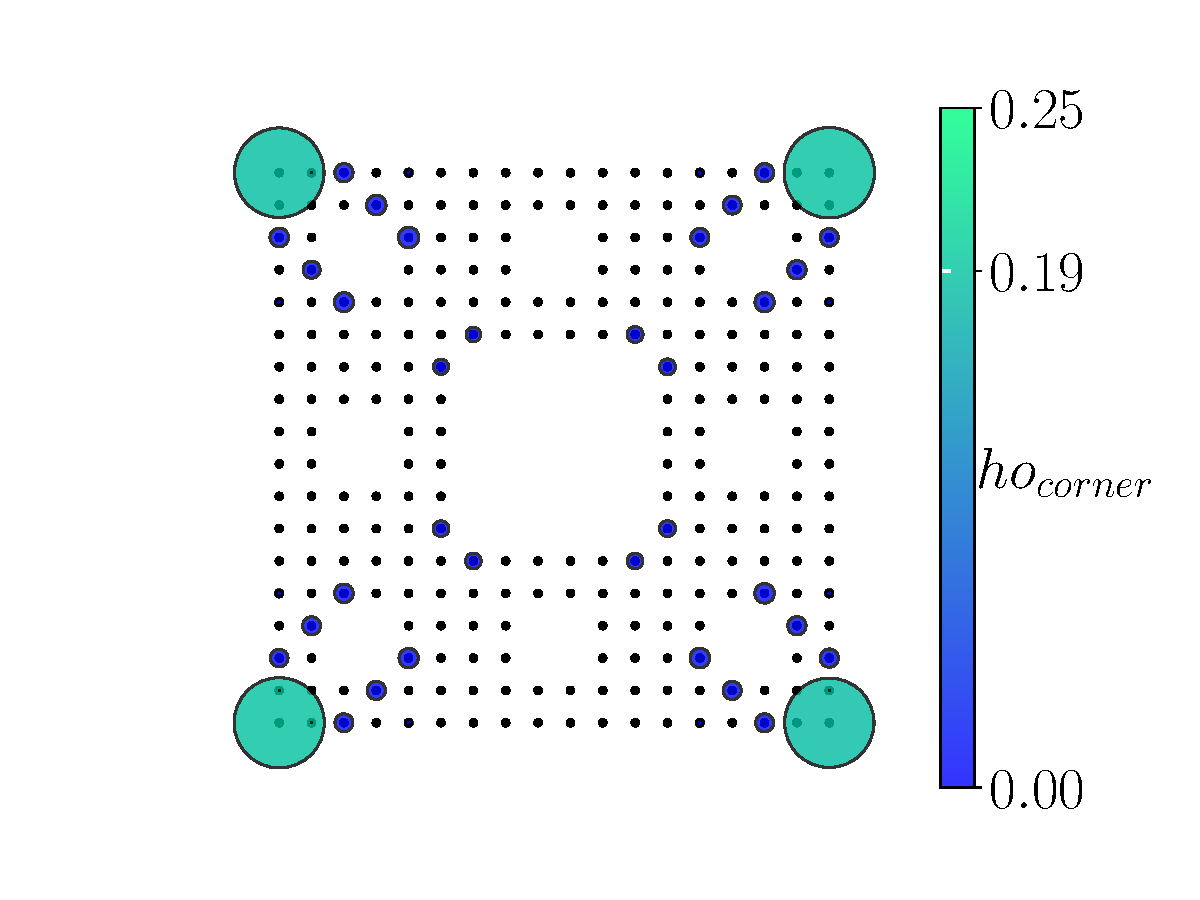
\includegraphics[width=\textwidth]{Imagenes/Resultados_Hoti_Fractal/proyection_square_0.05.pdf}
         \end{subfigure}\hspace*{-0.5em}
     \end{minipage}\vspace*{-1.5em}
     
     \begin{minipage}[h!]{0.9\textwidth}
         \begin{subfigure}[b!]{0.3 \textwidth}
            \caption{$\epsilon = 5\%$}             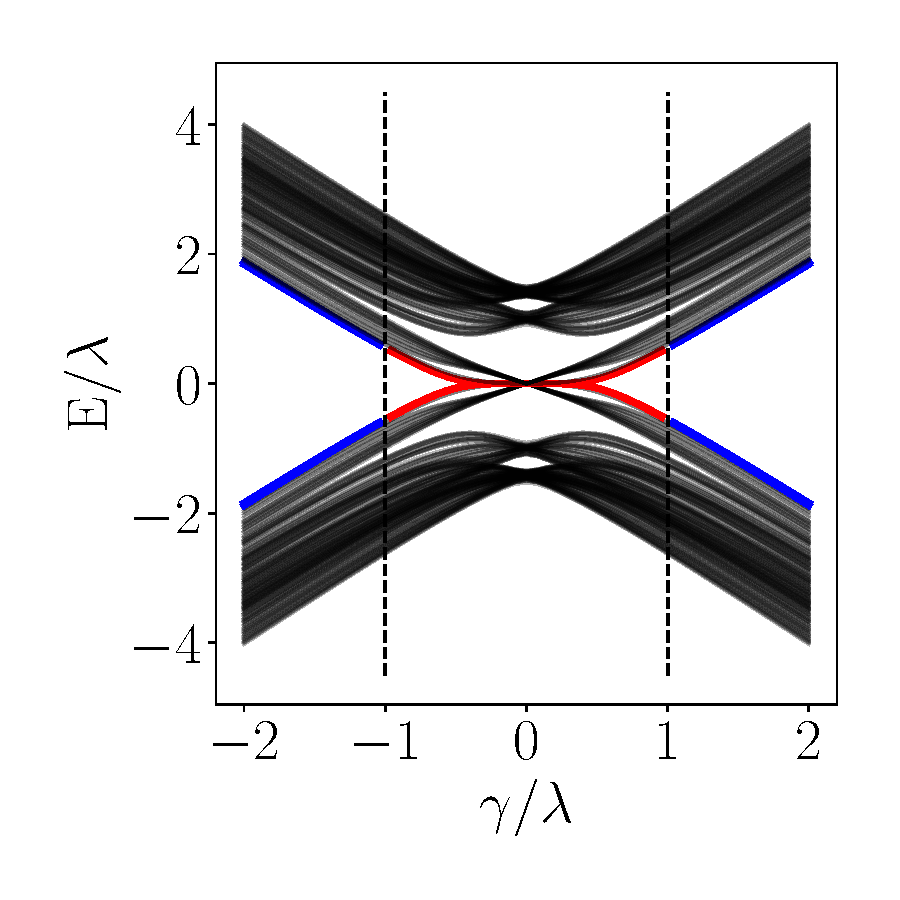
\includegraphics[width=\textwidth]{Imagenes/Resultados_Hoti_Fractal/bands_square_shh_0.1.pdf}
         \end{subfigure}\hspace*{-0.5em}
         \begin{subfigure}[b!]{0.3 \textwidth}
            \caption*{}
            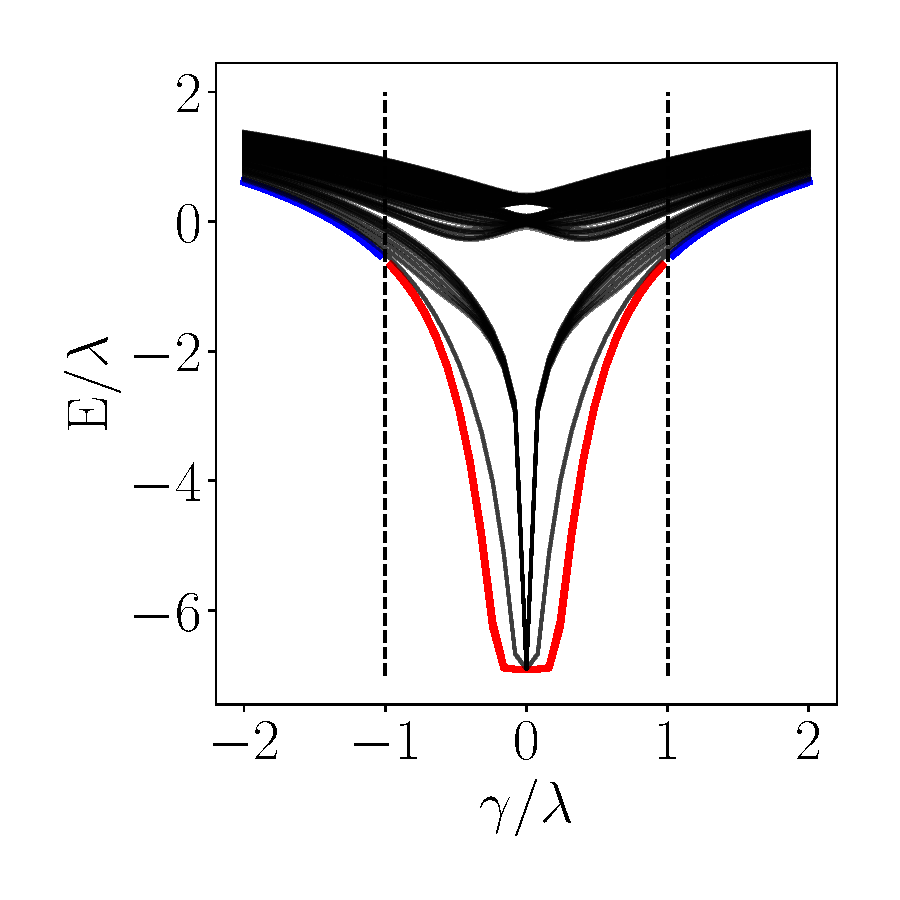
\includegraphics[width=\textwidth]{Imagenes/Resultados_Hoti_Fractal/bands_square_shh_log0.1.pdf}
         \end{subfigure}\hspace*{-0.5em}
         \begin{subfigure}[b!]{0.4 \textwidth}
            \caption*{}
            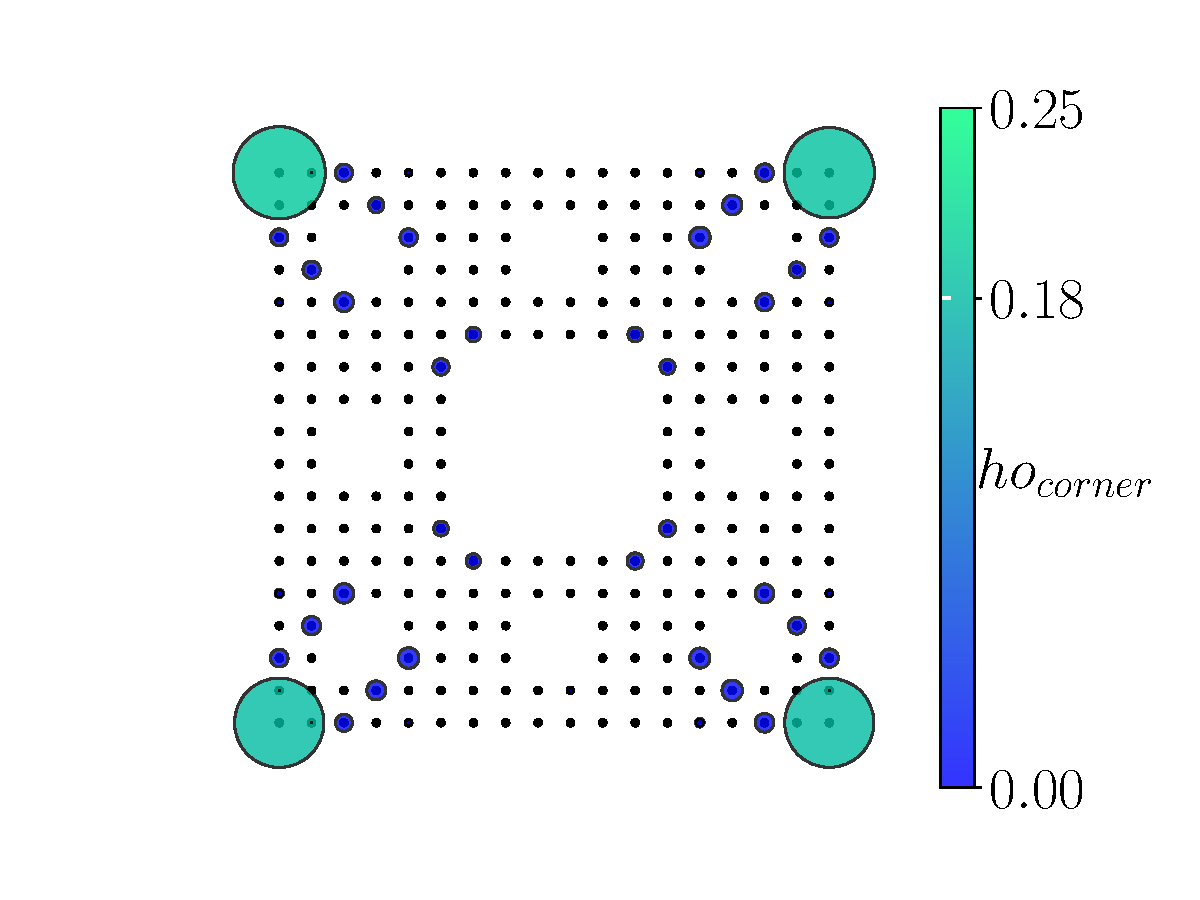
\includegraphics[width=\textwidth]{Imagenes/Resultados_Hoti_Fractal/proyection_square_0.1.pdf}
         \end{subfigure}\hspace*{-0.5em}
     \end{minipage}\vspace*{-1.5em}
     
     \begin{minipage}[h!]{0.9\textwidth}
         \begin{subfigure}[b!]{0.3 \textwidth}
            \caption{$\epsilon = 20\%$}             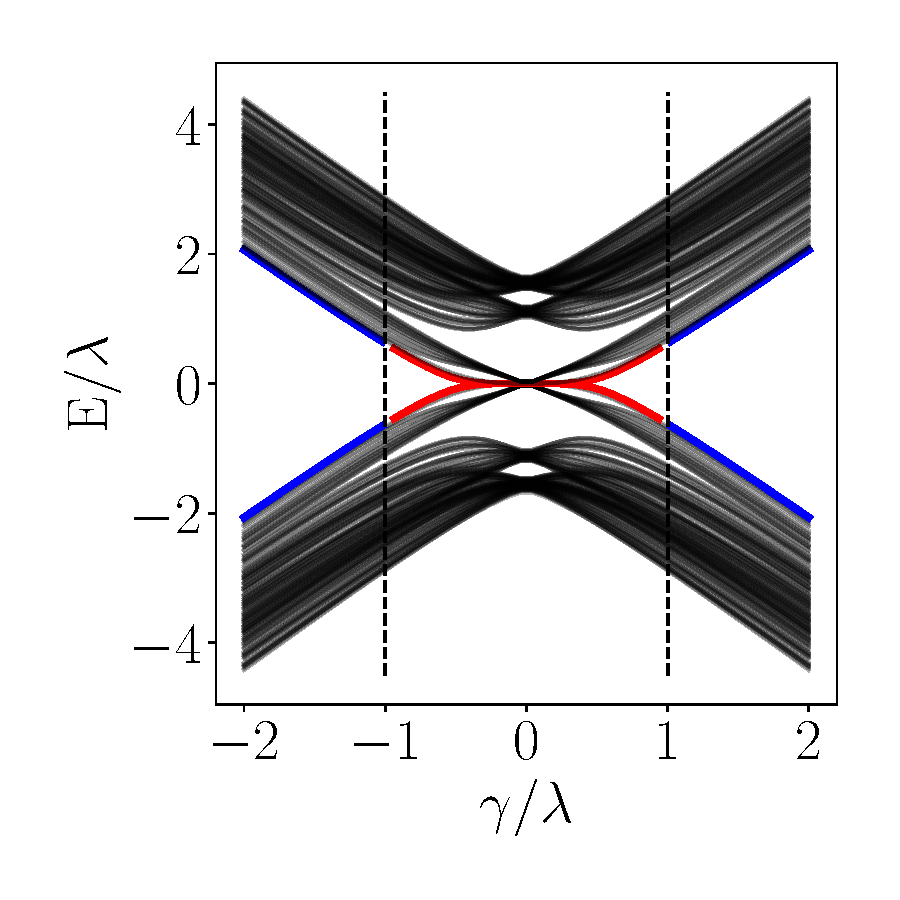
\includegraphics[width=\textwidth]{Imagenes/Resultados_Hoti_Fractal/bands_square_shh_0.2.pdf}
         \end{subfigure}\hspace*{-0.5em}
         \begin{subfigure}[b!]{0.3 \textwidth}
            \caption*{}
            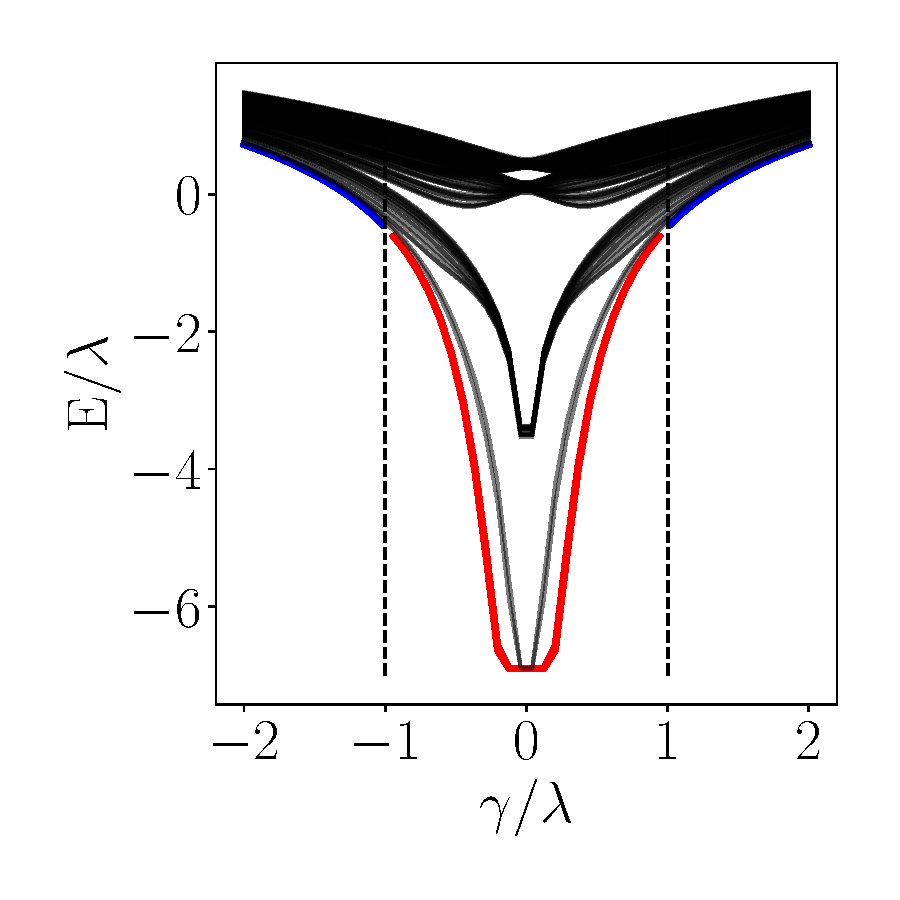
\includegraphics[width=\textwidth]{Imagenes/Resultados_Hoti_Fractal/bands_square_shh_log0.2.pdf}
         \end{subfigure}\hspace*{-0.5em}
         \begin{subfigure}[b!]{0.4 \textwidth}
            \caption*{}
            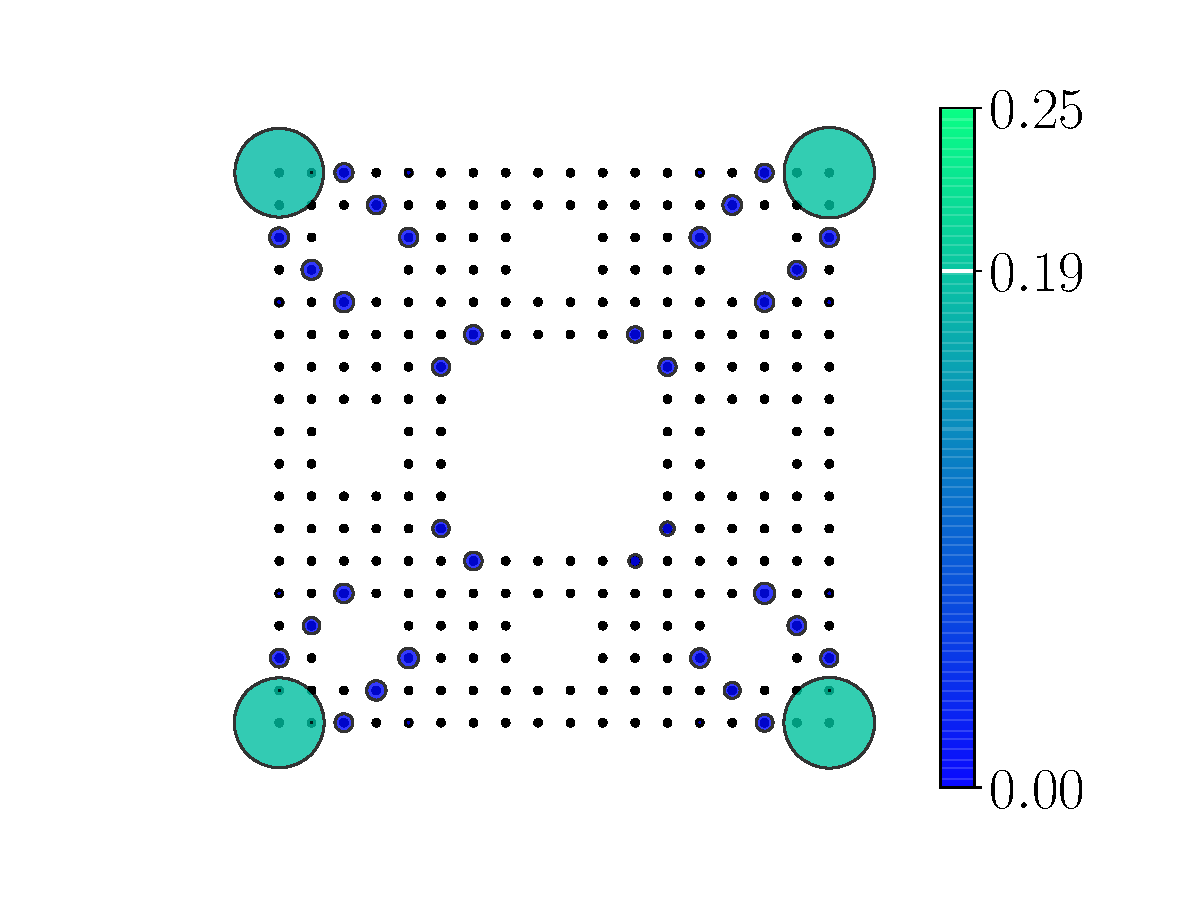
\includegraphics[width=\textwidth]{Imagenes/Resultados_Hoti_Fractal/proyection_square_0.2.pdf}
         \end{subfigure}\hspace*{-0.5em}
     \end{minipage}\vspace*{-1.5em}
     
     \begin{minipage}[h!]{0.9\textwidth}
         \begin{subfigure}[b!]{0.3 \textwidth}
            \caption{$\epsilon = 30\%$}             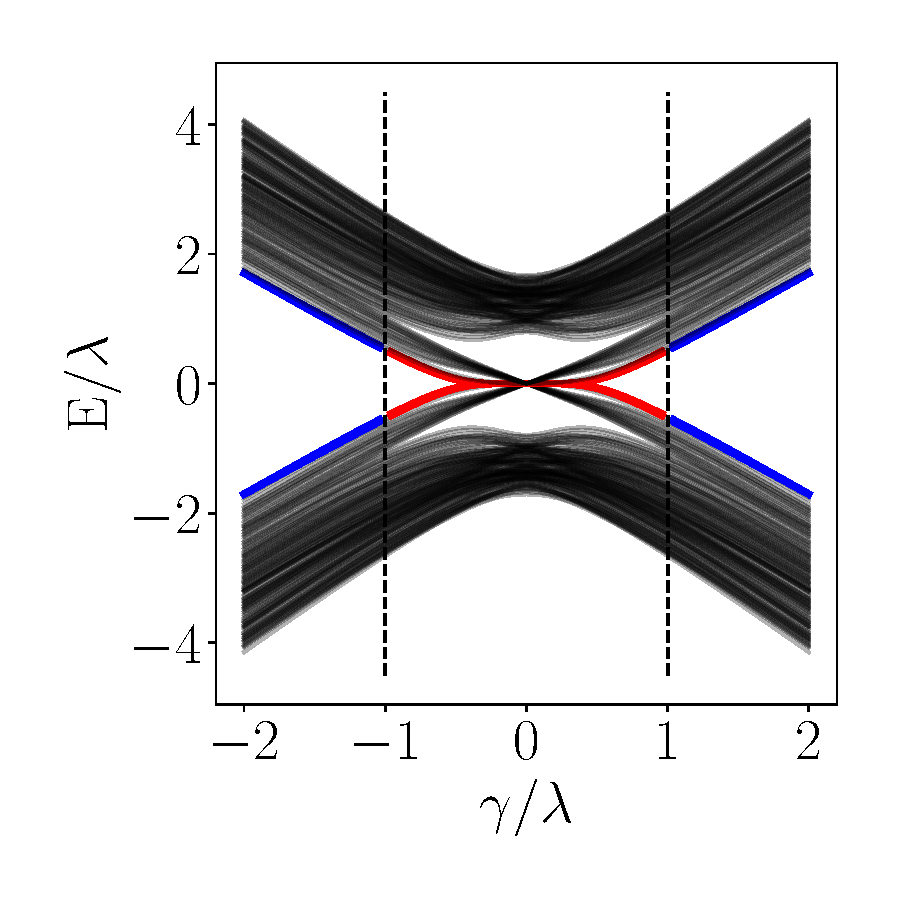
\includegraphics[width=\textwidth]{Imagenes/Resultados_Hoti_Fractal/bands_square_shh_0.3.pdf}
         \end{subfigure}\hspace*{-0.5em}
         \begin{subfigure}[b!]{0.3 \textwidth}
            \caption*{}
            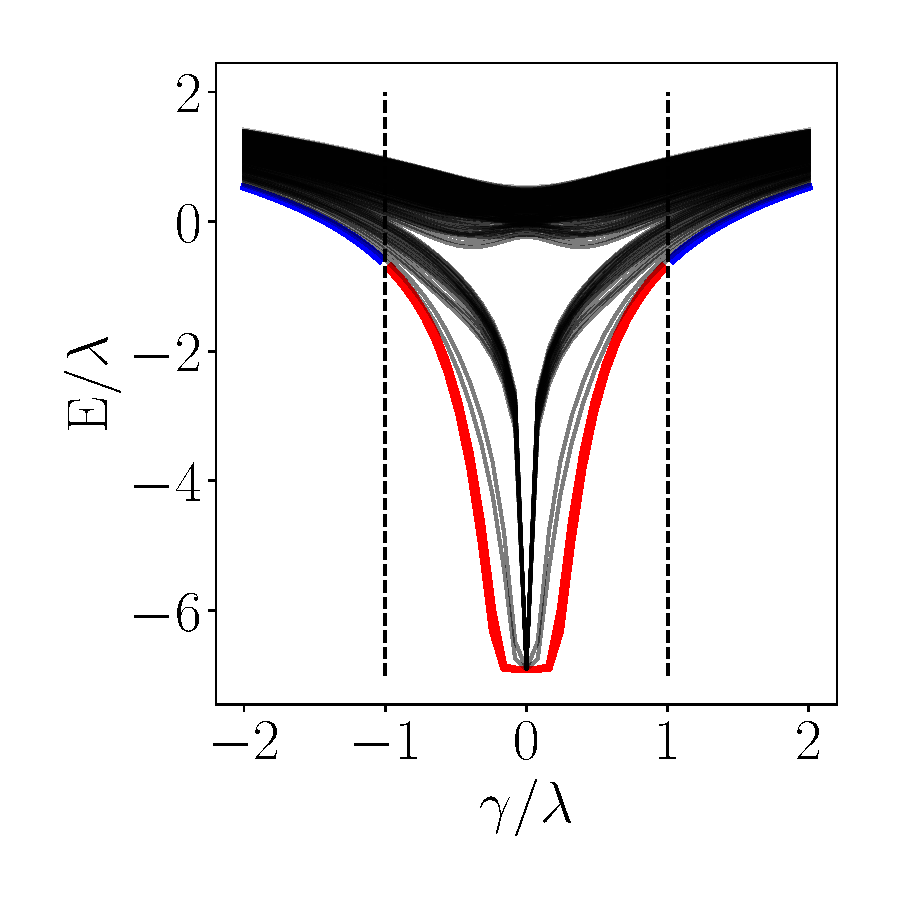
\includegraphics[width=\textwidth]{Imagenes/Resultados_Hoti_Fractal/bands_square_shh_log0.3.pdf}
         \end{subfigure}\hspace*{-0.5em}
         \begin{subfigure}[b!]{0.4 \textwidth}
            \caption*{}
            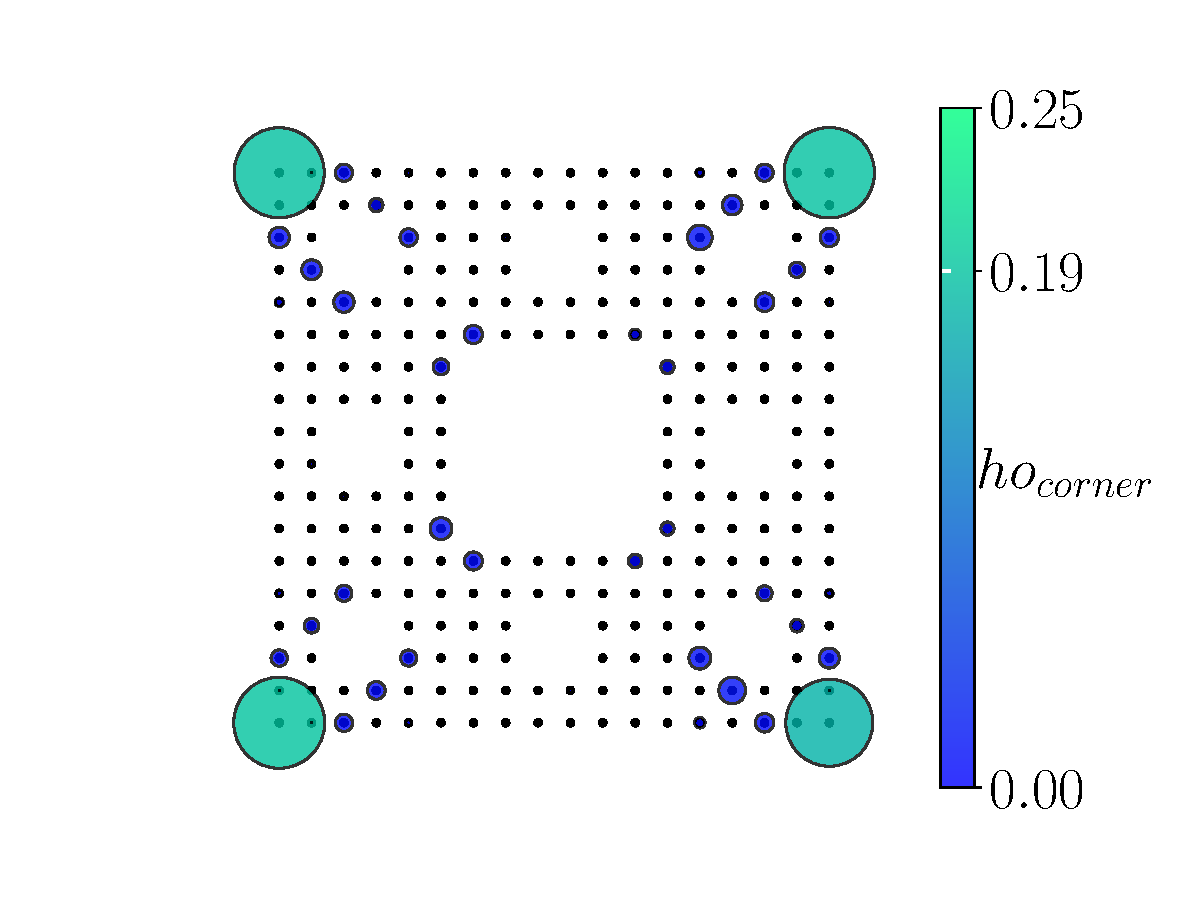
\includegraphics[width=\textwidth]{Imagenes/Resultados_Hoti_Fractal/proyection_square_0.3.pdf}
         \end{subfigure}\hspace*{-0.5em}
     \end{minipage}\vspace*{-1.5em}
     
      \begin{minipage}[h!]{0.9\textwidth}
         \begin{subfigure}[b!]{0.3 \textwidth}
            \caption{$\epsilon = 50\%$}             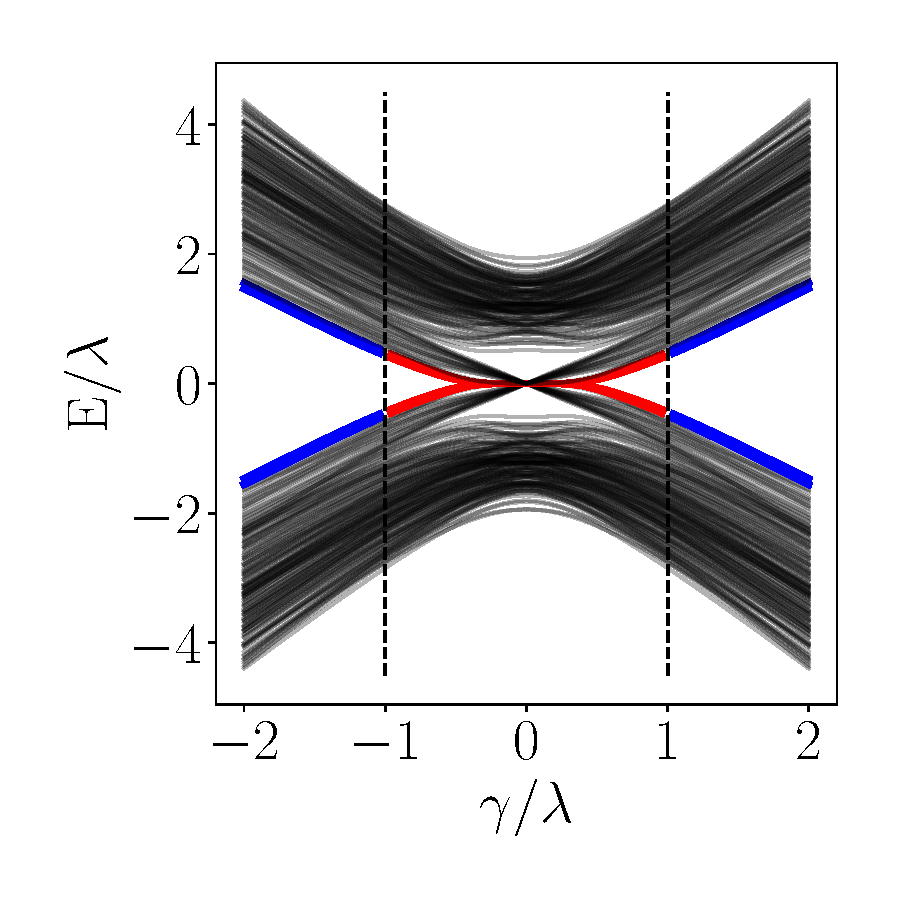
\includegraphics[width=\textwidth]{Imagenes/Resultados_Hoti_Fractal/bands_square_shh_0.5.pdf}
         \end{subfigure}\hspace*{-0.5em}
         \begin{subfigure}[b!]{0.3 \textwidth}
            \caption*{}
            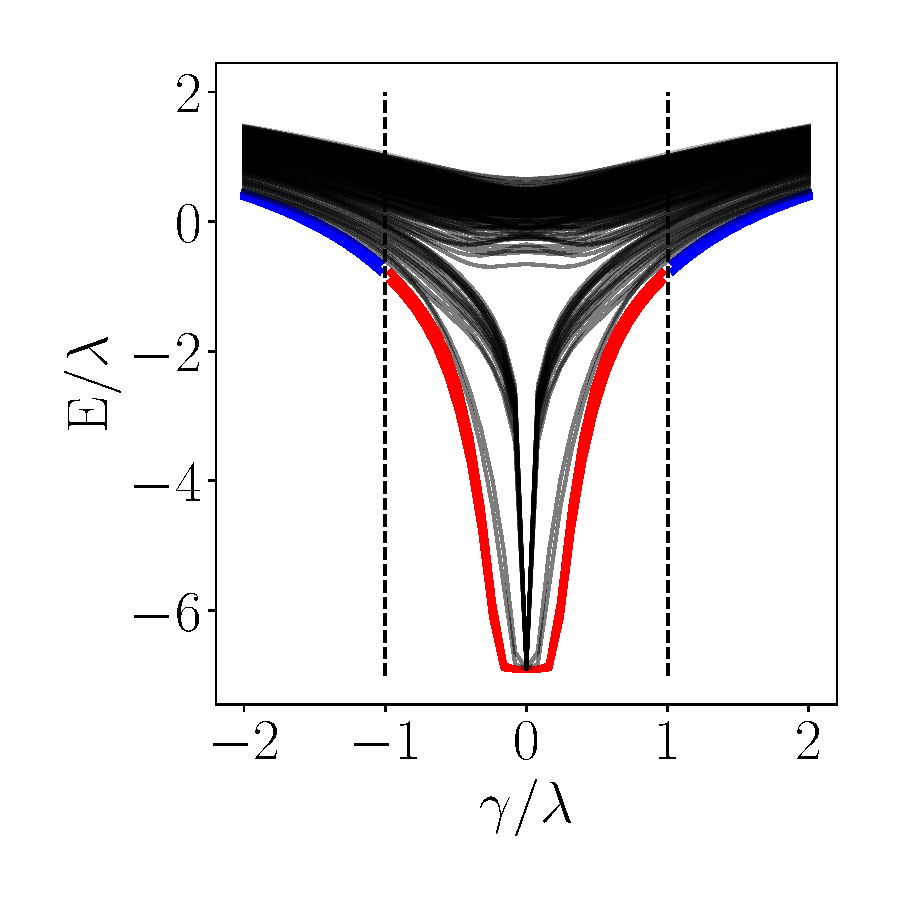
\includegraphics[width=\textwidth]{Imagenes/Resultados_Hoti_Fractal/bands_square_shh_log0.5.pdf}
         \end{subfigure}\hspace*{-0.5em}
         \begin{subfigure}[b!]{0.4 \textwidth}
             \caption*{}
             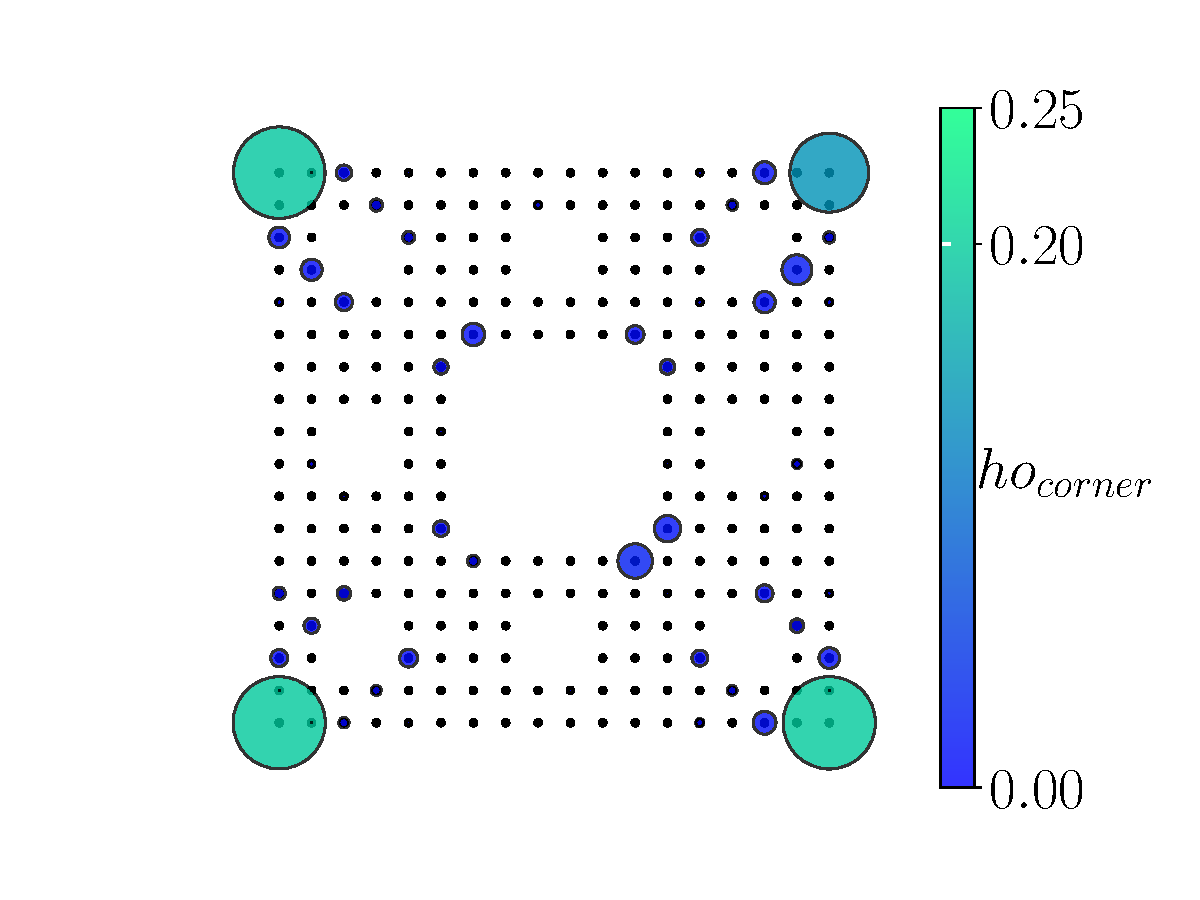
\includegraphics[width=\textwidth]{Imagenes/Resultados_Hoti_Fractal/proyection_square_0.5.pdf}
         \end{subfigure}\hspace*{-0.5em}
     \end{minipage}
     
     
    \caption{En la columna derecha se muestra el espectro de energías en una red cuadrada como función de $\gamma/\lambda $ con un desorden aleatorio en los parámetros de salto, de tamaño $\epsilon$. Las lineas rojas corresponden a los cuatro estados degenerados que representan los estados localizados en las esquinas. En la columna central se muestra el espectro de energías en escala logarítmica. En la columna izquierda se muestra la densidad de probabilidad de la fase no trivial donde $\gamma' = \gamma( 1 \pm \epsilon) ,\, \, \lambda' = \lambda( 1 \pm \epsilon)$.  }
    \label{fig:para_proy_Delta_fractal}
\end{figure}



\begin{figure}[h!]
    \centering
   \captionsetup[sub]{font=small}

    \begin{subfigure}[b!]{0.33 \textwidth}
        \caption{}
        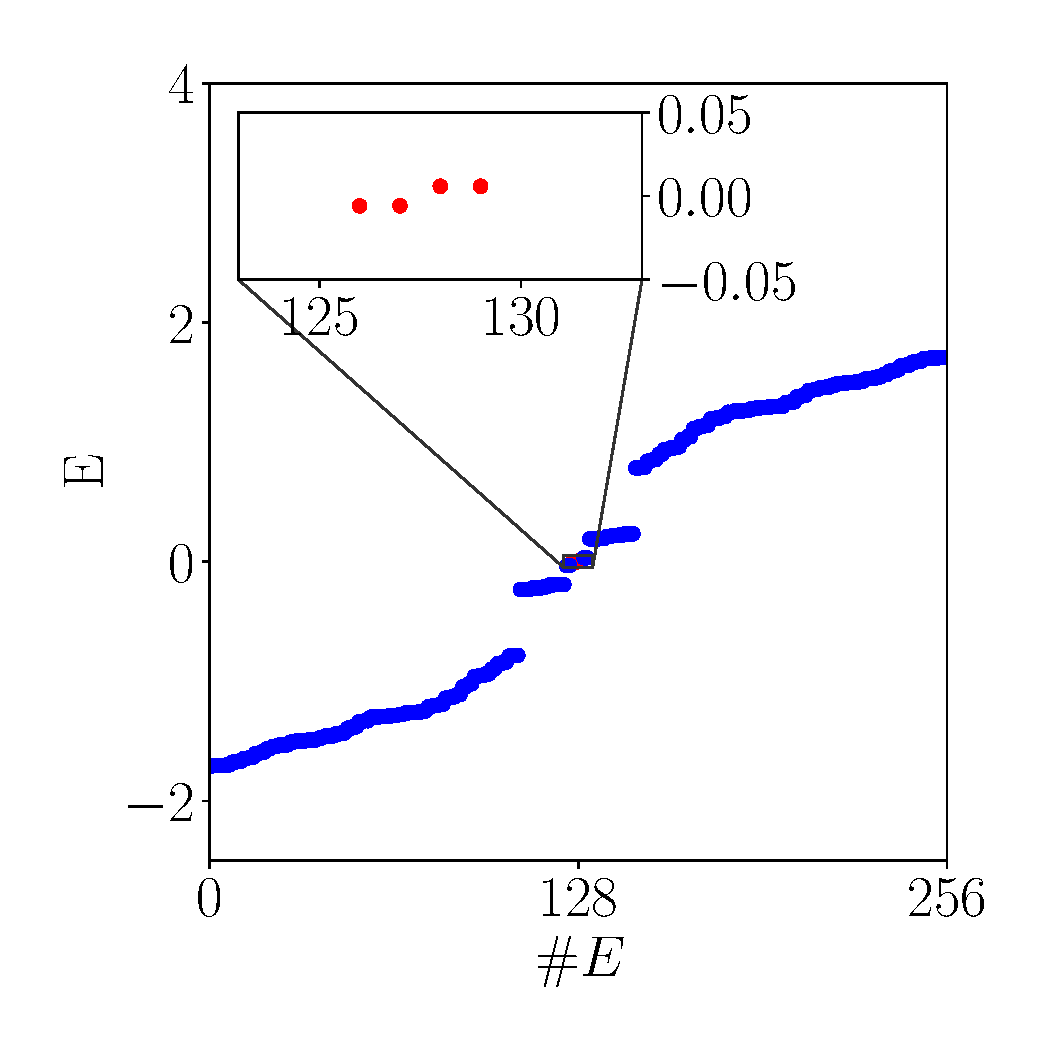
\includegraphics[width=\textwidth]{Imagenes/Resultados_Hoti_Fractal/spectre_square_fractal.pdf}
    \end{subfigure}
    \begin{subfigure}[b!]{0.33 \textwidth}
        \caption{}
        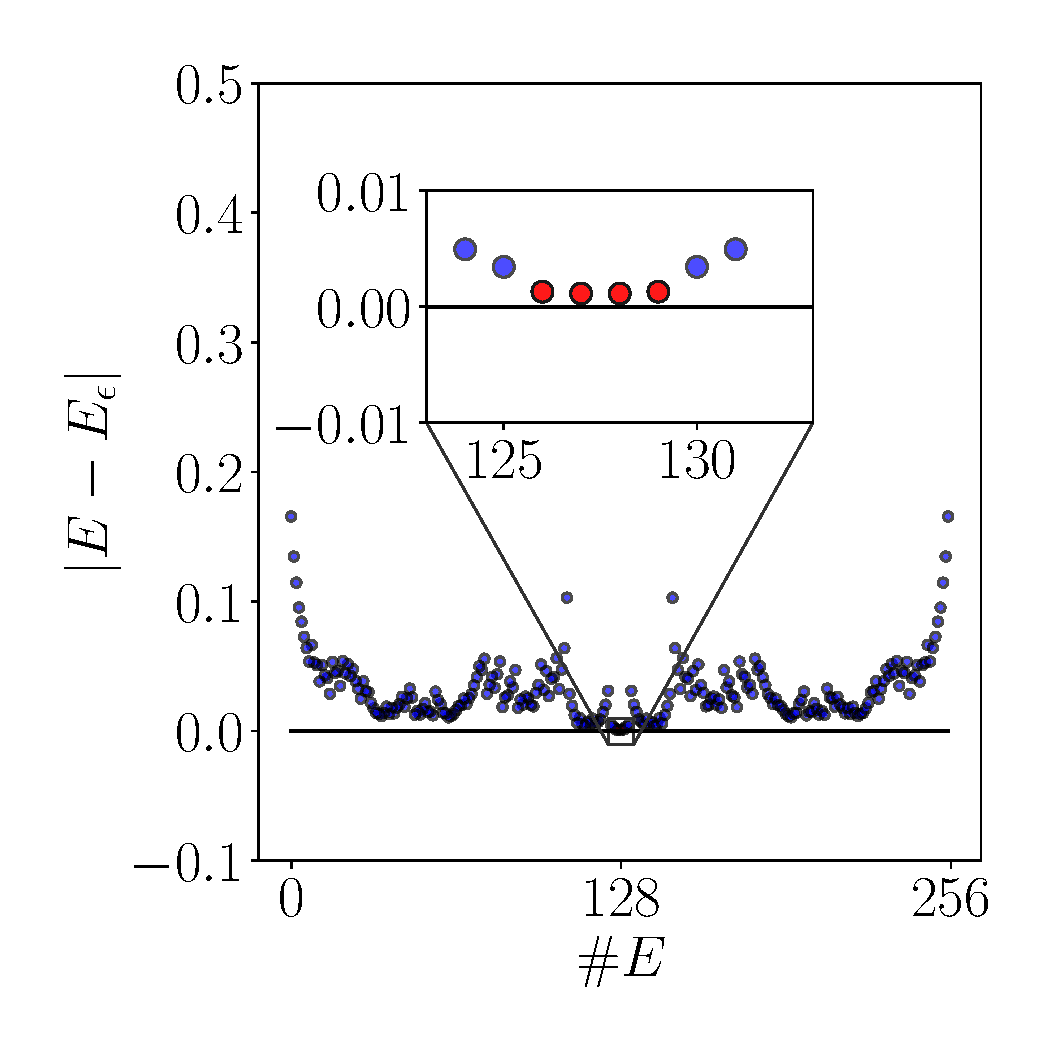
\includegraphics[width=\textwidth]{Imagenes/Resultados_Hoti_Fractal/spectre_square_epsi_fractal.pdf} 
    \end{subfigure}
    \begin{subfigure}[b!]{0.33 \textwidth}
        \caption{}
        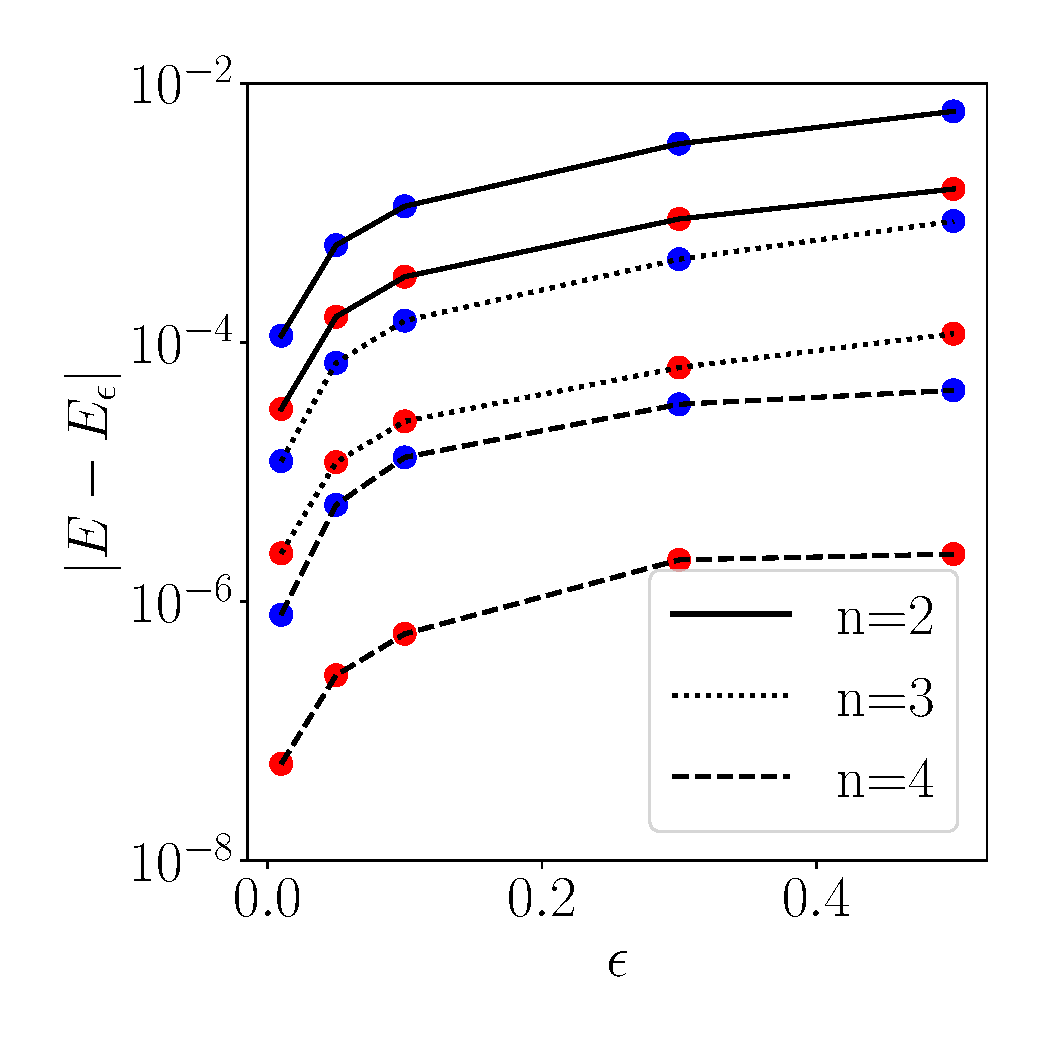
\includegraphics[width=\textwidth]{Imagenes/Resultados_Hoti_Fractal/pertubation_gen_fractal.pdf}
    \end{subfigure}\hspace*{-0.9em}

       \caption{\textbf{(a)} Espectro de energias odenadas para la red Sierpinski con $\gamma = 0.5$ y $\lambda = 1.0$. \textbf{(b)} Cambio del espectro de energias cuando se perturban los parametros de salto con $\epsilon = 30\%$.}
       \label{fig:spectre_fractal_epsi}
\end{figure}

\section{Bombeo en un red cuadrada y en una alfombra de Sierpinski}

Como se mencionó en la introducción existen trabajos recientes que muestran que las propiedades de transporte en aislantes topológicos de pueden presentar con estados protegidos por invariantes como el número de Chern. En el artículo \textit{High order topological pump}\cite{benalcazar2020higher}, Benalcazar at al. muestran estas propiedades en un arreglo experimental con guías de ondas. Inspirados en esta idea decidimos introducir parámetros cíclicos similares a los de una onda evanecente de guía de onda a nuestro modelo anterio de BBH en el Hoti cuadrado y fractal, para lo cual haremos un cambio en los parametros de salto como se muestra en la ecuacion \ref{eq:param_pump}. El parámetro de sitio $\epsilon_0 \apprx \pm 0.5$ toma el signo como se muestra en la figura \ref{fig:Models} \textbf{(a)}, este parametro rompe la simetría de espejo y permite que el moviemiento de los centros de wannier suceda de forma adiabática.

\begin{align}
    \label{eq:param_pump}
    \nonumber\gamma \rightarrow \gamma (\theta) = \gamma_0 e^{\displaystyle-\beta(1 - A \cos \theta )} \; &,\;  \lambda \rightarrow \lambda(\theta) = \lambda_0 e^{\displaystyle-\beta( 1 + A \cos \theta )} \;,\; \\  \epsilon(\theta) &= \epsilon_0 \sin \theta
\end{align}

Estas variaciones ciclicas se realizaron sobre diferentes direcciones en los parametros de nuestras redes: 

\begin{align}
    \label{eq:param_pumpxy}
    \nonumber \gamma_x = \gamma_y = \gamma (\theta) = \gamma_0 e^{\displaystyle-\beta(1 - A \cos \theta )} \\ \lambda_x = \lambda_y = \lambda(\theta) = \lambda_0 e^{\displaystyle-\beta( 1 + A \cos \theta )}
\end{align}
\begin{align}
    \label{eq:param_pumpx}
    \nonumber \gamma_x =\gamma_0 \; &,\; \gamma_y = \gamma (\theta) = \gamma_0 e^{\displaystyle-\beta(1 - A \cos \theta )} \\
    \lambda_x = \lambda_0  \; &,\;  \lambda_y = \lambda(\theta) = \lambda_0 e^{\displaystyle-\beta( 1 + A \cos \theta )}
\end{align}
\begin{align}
    \label{eq:param_pumpy}
    \nonumber \gamma_x = \gamma (\theta) = \gamma_0 e^{\displaystyle-\beta(1 - A \cos \theta )}   \; &,\; \gamma_x =\gamma_0 \\
    \lambda_y = \lambda(\theta) = \lambda_0 e^{\displaystyle-\beta( 1 + A \cos \theta )} \; &,\; \lambda_x = \lambda_0  
\end{align}

Las variciones en los ejes $\mathbf{X}$ y $\mathbf{Y}$ (eq. \ref{eq:param_pumpxy})


Las variciones en el eje $\mathbf{X}$ (eq. \ref{eq:param_pumpx})


Las variciones en el eje $\mathbf{Y}$ (eq. \ref{eq:param_pumpy})

Los moviemientos que generan las variaciones de los parametros de salto sobre la red se pueden observar en la Figura \ref{fig:Model_pump} \textbf{(a)-(f)}, respectivamente.


 %\renewcommand{\thesubfigure}{\roman{subfigure}}
\begin{figure}[h!]
     \centering
    \captionsetup[sub]{font=small}
     \begin{minipage}[h!]{1\textwidth}
         \begin{subfigure}[b!]{0.2 \textwidth}
             \caption{$\theta = - \pi$}
             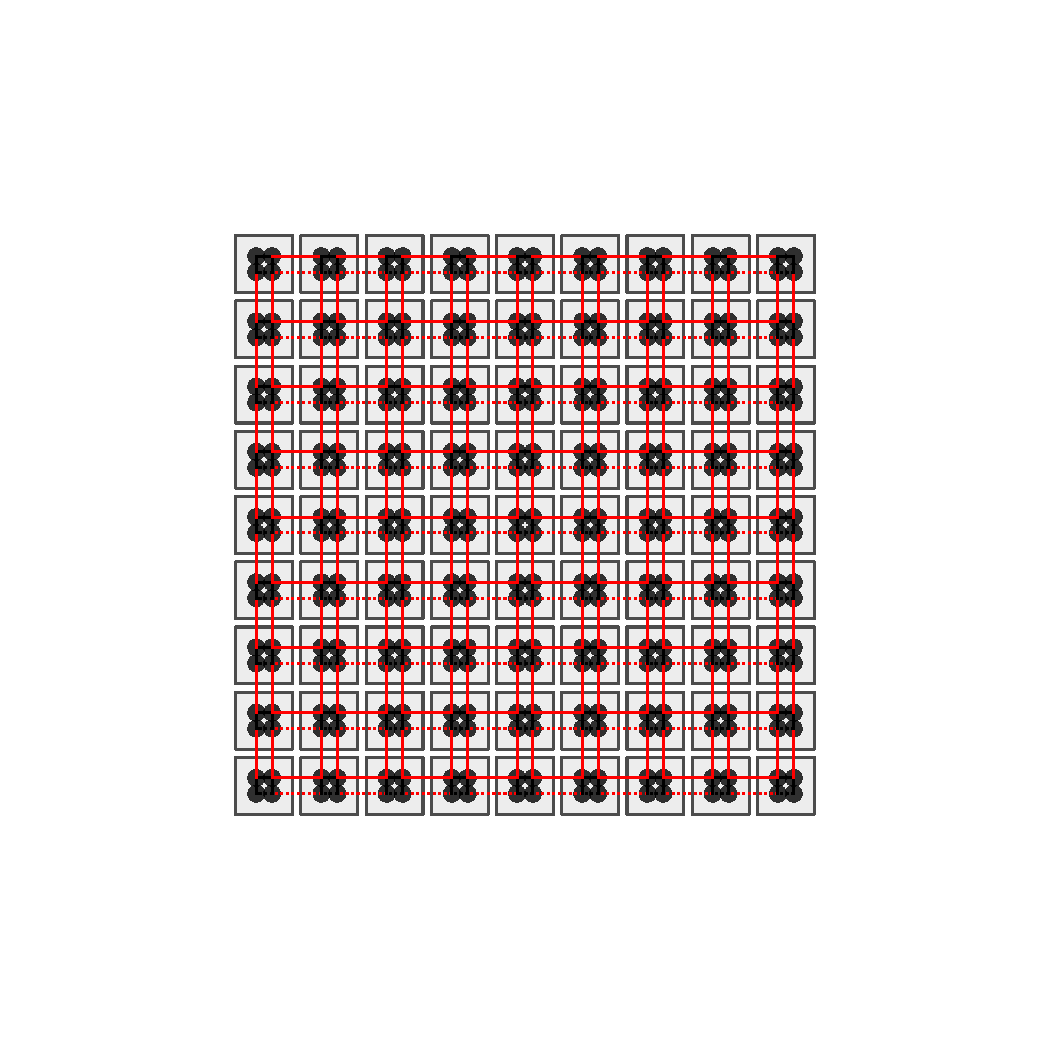
\includegraphics[width=\textwidth]{Imagenes/Models/Model_pump/square_pump_model_xy_0.pdf}
         \end{subfigure}\hspace*{-0.5em}
         \begin{subfigure}[b!]{0.2 \textwidth}
             \caption*{$\theta = -\frac{\pi}{2}$}
             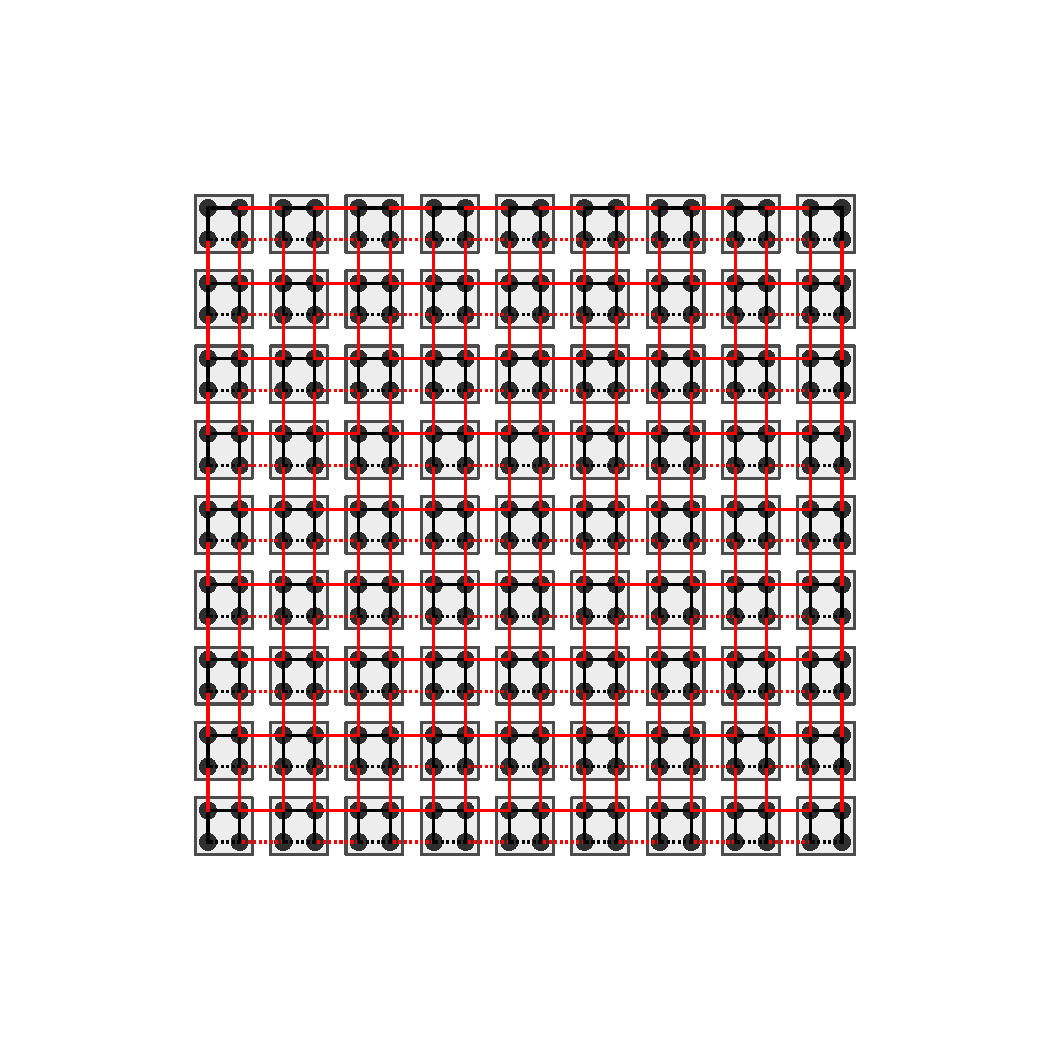
\includegraphics[width=\textwidth]{Imagenes/Models/Model_pump/square_pump_model_xy_5.pdf}
         \end{subfigure}\hspace*{-0.5em}
         \begin{subfigure}[b!]{0.2 \textwidth}
             \caption*{$\theta = 0$}
             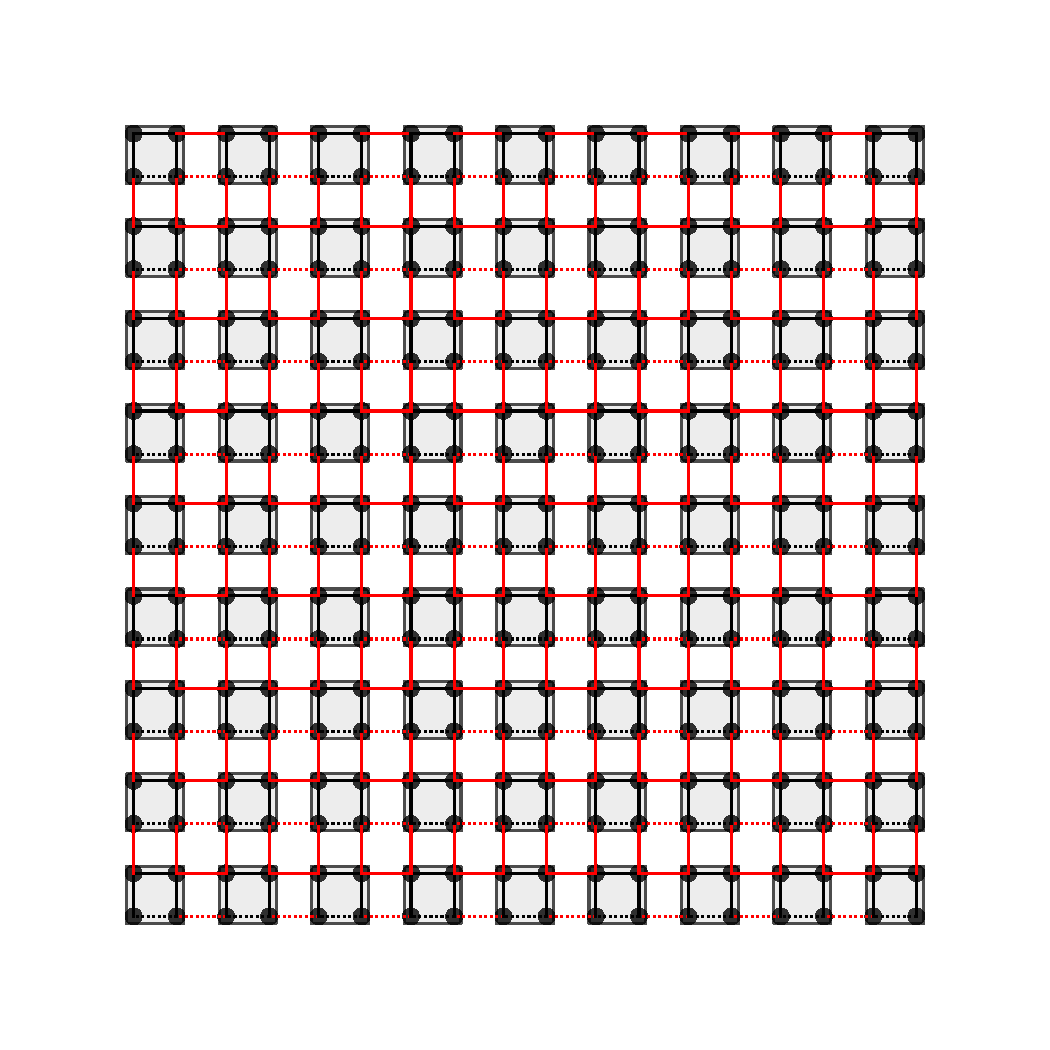
\includegraphics[width=\textwidth]{Imagenes/Models/Model_pump/square_pump_model_xy_8.pdf}
         \end{subfigure}\hspace*{-0.5em}
         \begin{subfigure}[b!]{0.2 \textwidth}
             \caption*{$\theta = \frac{\pi}{2}$}
             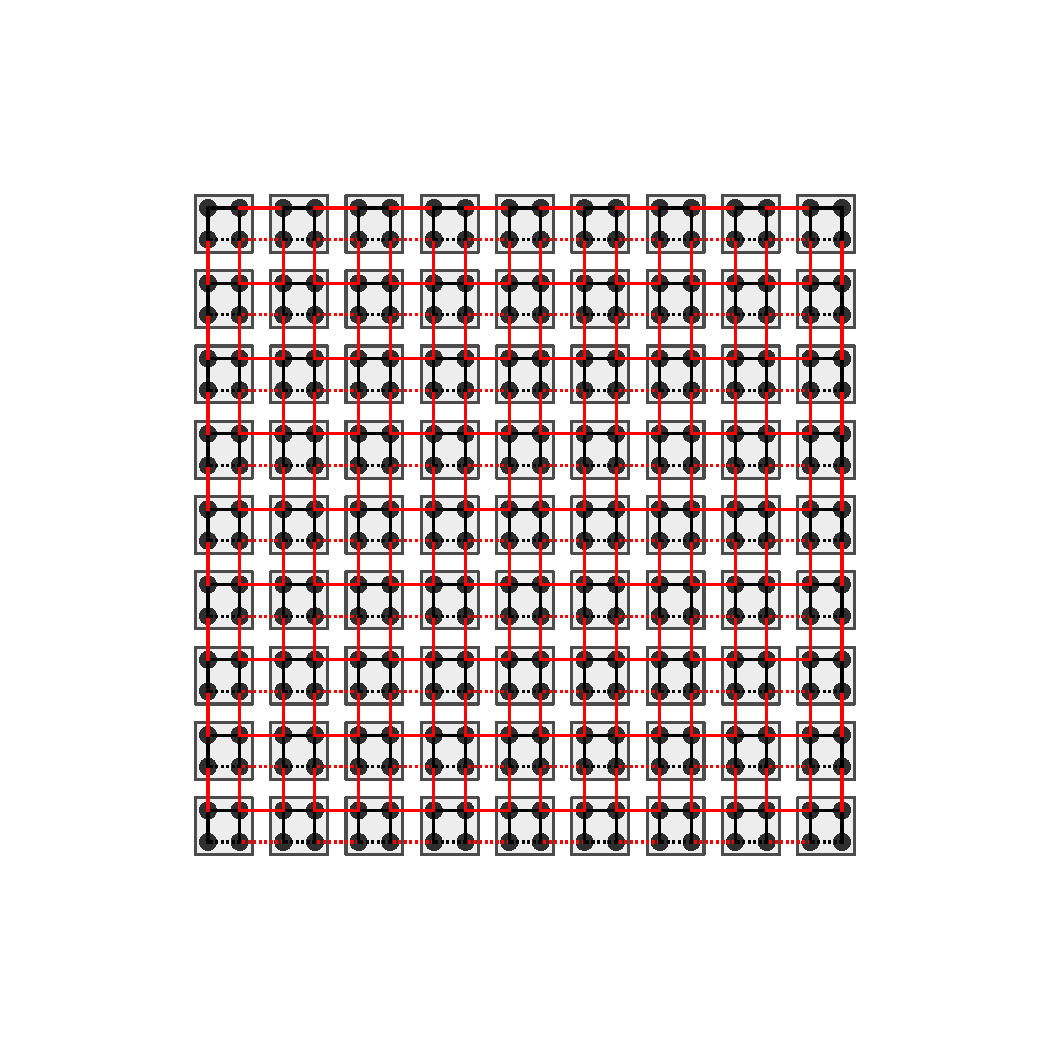
\includegraphics[width=\textwidth]{Imagenes/Models/Model_pump/square_pump_model_xy_11.pdf}
         \end{subfigure}\hspace*{-0.5em}
         \begin{subfigure}[b!]{0.2 \textwidth}
             \caption*{$\theta = \pi$}
             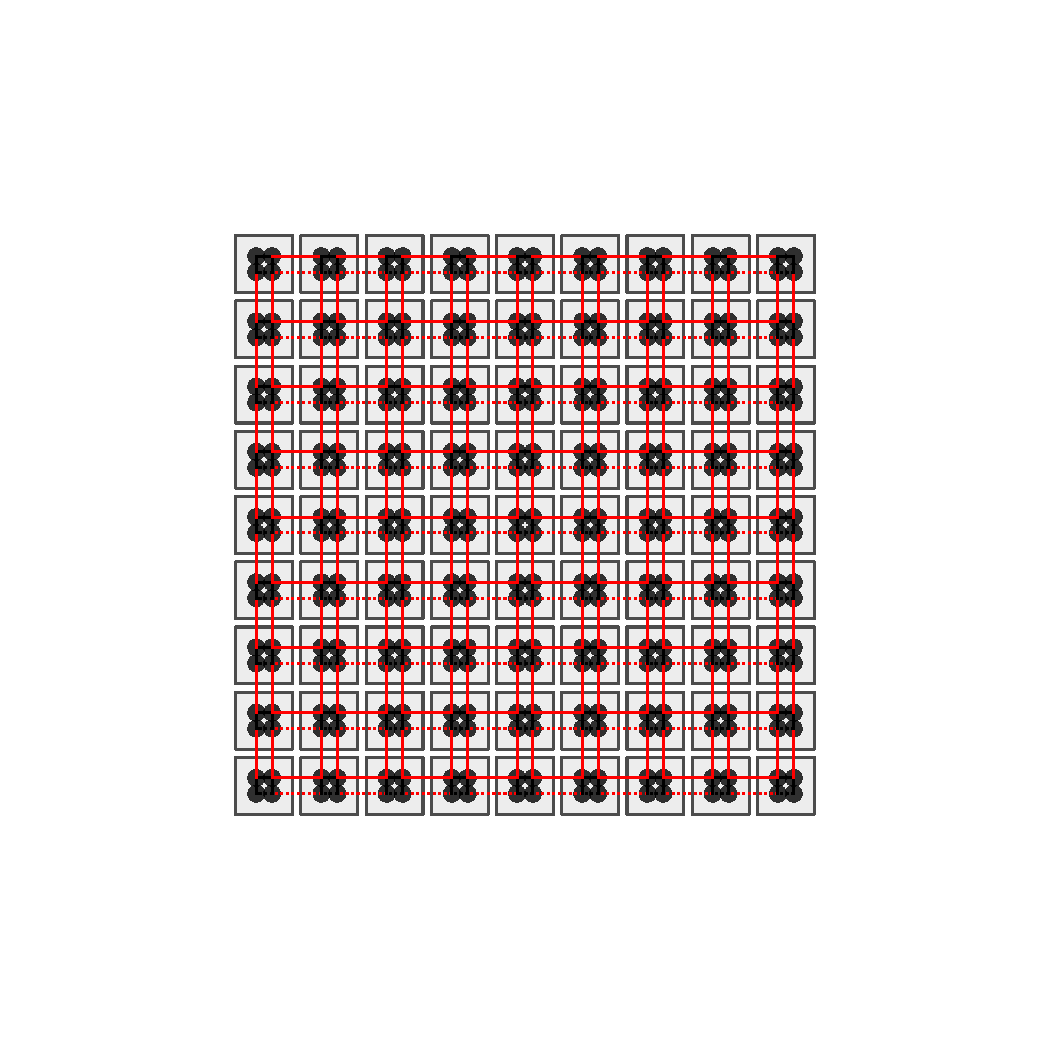
\includegraphics[width=\textwidth]{Imagenes/Models/Model_pump/square_pump_model_xy_16.pdf}
         \end{subfigure}\hspace*{-0.5em}
     \end{minipage}\vspace*{-1em}
     
     
     \begin{minipage}[h!]{1\textwidth}
         \begin{subfigure}[b!]{0.2 \textwidth}
             \caption{}
             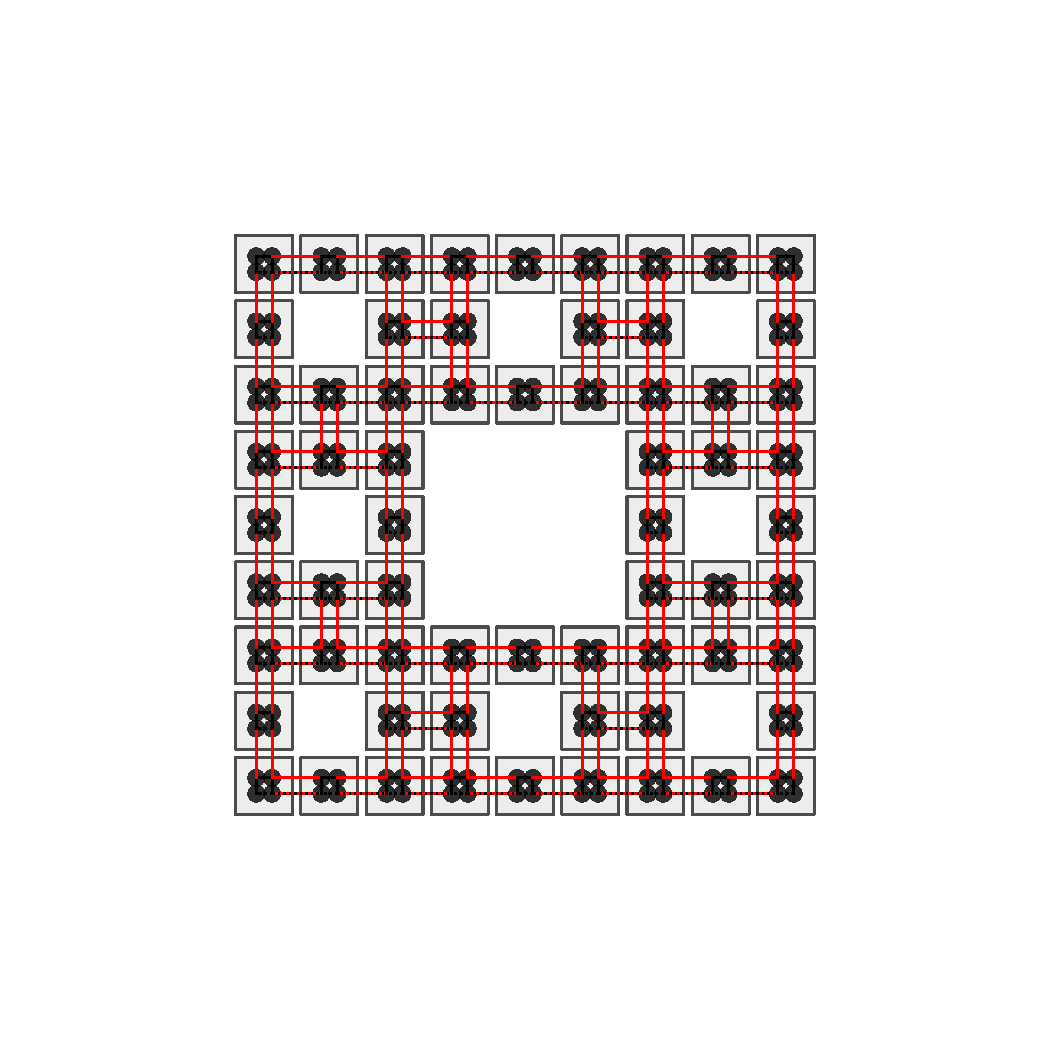
\includegraphics[width=\textwidth]{Imagenes/Models/Model_pump/fractal_pump_model_xy_0.pdf}
         \end{subfigure}\hspace*{-0.5em}
         \begin{subfigure}[b!]{0.2 \textwidth}
             \caption*{}
             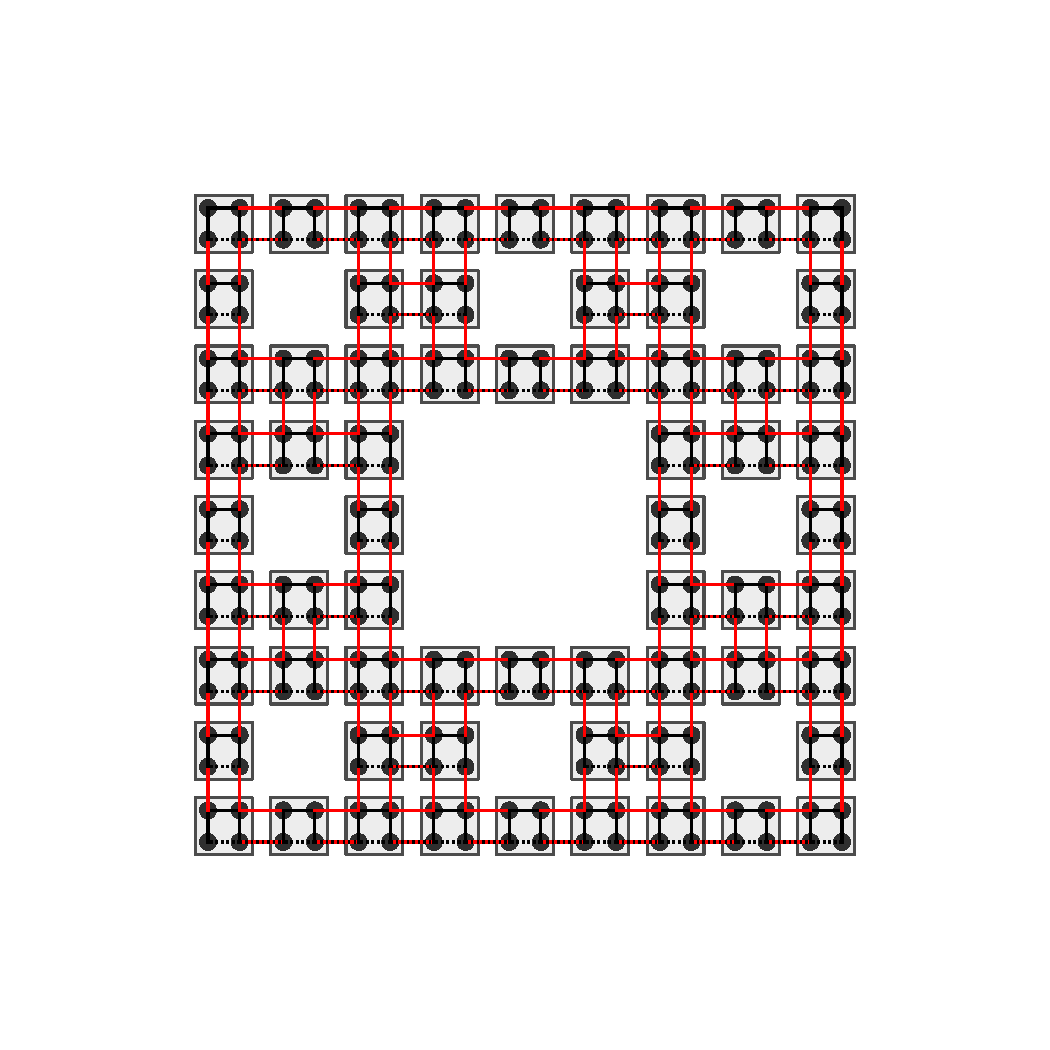
\includegraphics[width=\textwidth]{Imagenes/Models/Model_pump/fractal_pump_model_xy_5.pdf}
         \end{subfigure}\hspace*{-0.5em}
         \begin{subfigure}[b!]{0.2 \textwidth}
             \caption*{}
             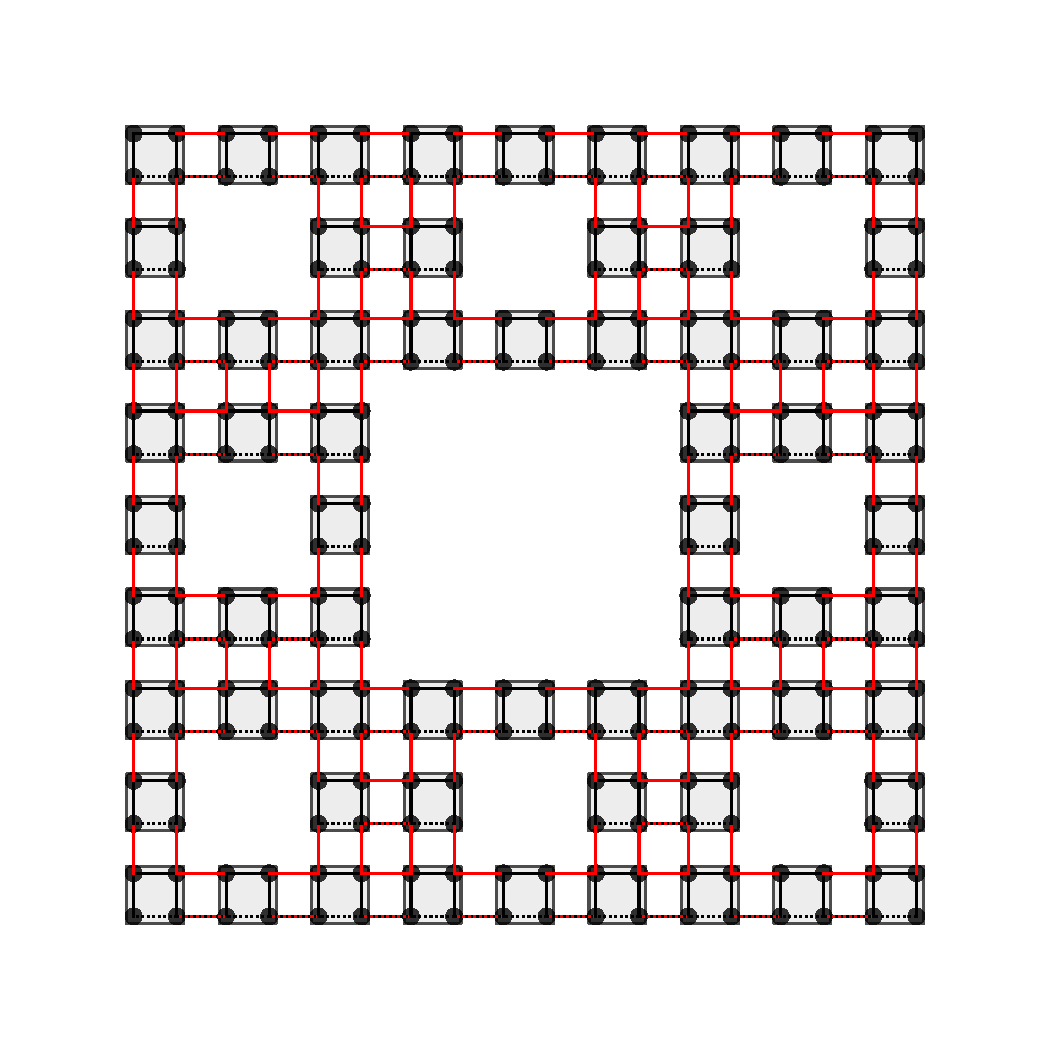
\includegraphics[width=\textwidth]{Imagenes/Models/Model_pump/fractal_pump_model_xy_8.pdf}
         \end{subfigure}\hspace*{-0.5em}
         \begin{subfigure}[b!]{0.2 \textwidth}
             \caption*{}
             \includegraphics[width=\textwidth]{Imagenes/Models/Model_pump/fractal_pump_model_xy_11.pdf}
         \end{subfigure}\hspace*{-0.5em}
         \begin{subfigure}[b!]{0.2 \textwidth}
             \caption*{}
             \includegraphics[width=\textwidth]{Imagenes/Models/Model_pump/fractal_pump_model_xy_16.pdf}
         \end{subfigure}\hspace*{-0.5em}
     \end{minipage}\vspace*{-1em}
     
     
     \begin{minipage}[h!]{1.0\textwidth}
         \begin{subfigure}[b!]{0.2 \textwidth}
             \caption{}
             \includegraphics[width=\textwidth]{Imagenes/Models/Model_pump/square_pump_model_x_0.pdf}
         \end{subfigure}\hspace*{-0.5em}
         \begin{subfigure}[b!]{0.2 \textwidth}
             \caption*{}
             \includegraphics[width=\textwidth]{Imagenes/Models/Model_pump/square_pump_model_x_5.pdf}
         \end{subfigure}\hspace*{-0.5em}
         \begin{subfigure}[b!]{0.2 \textwidth}
             \caption*{}
             \includegraphics[width=\textwidth]{Imagenes/Models/Model_pump/square_pump_model_x_8.pdf}
         \end{subfigure}\hspace*{-0.5em}
         \begin{subfigure}[b!]{0.2 \textwidth}
             \caption*{}
             \includegraphics[width=\textwidth]{Imagenes/Models/Model_pump/square_pump_model_x_11.pdf}
         \end{subfigure}\hspace*{-0.5em}
         \begin{subfigure}[b!]{0.2 \textwidth}
             \caption*{}
             \includegraphics[width=\textwidth]{Imagenes/Models/Model_pump/square_pump_model_x_16.pdf}
         \end{subfigure}\hspace*{-0.5em}
     \end{minipage}\vspace*{-1em}
     
     
     \begin{minipage}[h!]{1.0\textwidth}
         \begin{subfigure}[b!]{0.2 \textwidth}
             \caption{}
             \includegraphics[width=\textwidth]{Imagenes/Models/Model_pump/fractal_pump_model_x_0.pdf}
         \end{subfigure}\hspace*{-0.5em}
         \begin{subfigure}[b!]{0.2 \textwidth}
             \caption*{}
             \includegraphics[width=\textwidth]{Imagenes/Models/Model_pump/fractal_pump_model_x_5.pdf}
         \end{subfigure}\hspace*{-0.5em}
         \begin{subfigure}[b!]{0.2 \textwidth}
             \caption*{}
             \includegraphics[width=\textwidth]{Imagenes/Models/Model_pump/fractal_pump_model_x_8.pdf}
         \end{subfigure}\hspace*{-0.5em}
         \begin{subfigure}[b!]{0.2 \textwidth}
             \caption*{}
             \includegraphics[width=\textwidth]{Imagenes/Models/Model_pump/fractal_pump_model_x_11.pdf}
         \end{subfigure}\hspace*{-0.5em}
         \begin{subfigure}[b!]{0.2 \textwidth}
             \caption*{}
             \includegraphics[width=\textwidth]{Imagenes/Models/Model_pump/fractal_pump_model_x_16.pdf}
         \end{subfigure}\hspace*{-0.5em}
     \end{minipage}\vspace*{-1em}
     
     \begin{minipage}[h!]{1.0\textwidth}
         \begin{subfigure}[b!]{0.2 \textwidth}
             \caption{}
             \includegraphics[width=\textwidth]{Imagenes/Models/Model_pump/square_pump_model_y_0.pdf}
         \end{subfigure}\hspace*{-0.5em}
         \begin{subfigure}[b!]{0.2 \textwidth}
             \caption*{}
             \includegraphics[width=\textwidth]{Imagenes/Models/Model_pump/square_pump_model_y_5.pdf}
         \end{subfigure}\hspace*{-0.5em}
         \begin{subfigure}[b!]{0.2 \textwidth}
             \caption*{}
             \includegraphics[width=\textwidth]{Imagenes/Models/Model_pump/square_pump_model_y_8.pdf}
         \end{subfigure}\hspace*{-0.5em}
         \begin{subfigure}[b!]{0.2 \textwidth}
             \caption*{}
             \includegraphics[width=\textwidth]{Imagenes/Models/Model_pump/square_pump_model_y_11.pdf}
         \end{subfigure}\hspace*{-0.5em}
         \begin{subfigure}[b!]{0.2 \textwidth}
             \caption*{}
             \includegraphics[width=\textwidth]{Imagenes/Models/Model_pump/square_pump_model_y_16.pdf}
         \end{subfigure}\hspace*{-0.5em}
     \end{minipage}\vspace*{-1em}
     
     
     \begin{minipage}[h!]{1.0\textwidth}
         \begin{subfigure}[b!]{0.2 \textwidth}
             \caption{}
             \includegraphics[width=\textwidth]{Imagenes/Models/Model_pump/fractal_pump_model_y_0.pdf}
         \end{subfigure}\hspace*{-0.5em}
         \begin{subfigure}[b!]{0.2 \textwidth}
             \caption*{}
             \includegraphics[width=\textwidth]{Imagenes/Models/Model_pump/fractal_pump_model_y_5.pdf}
         \end{subfigure}\hspace*{-0.5em}
         \begin{subfigure}[b!]{0.2 \textwidth}
             \caption*{}
             \includegraphics[width=\textwidth]{Imagenes/Models/Model_pump/fractal_pump_model_y_8.pdf}
         \end{subfigure}\hspace*{-0.5em}
         \begin{subfigure}[b!]{0.2 \textwidth}
             \caption*{}
             \includegraphics[width=\textwidth]{Imagenes/Models/Model_pump/fractal_pump_model_y_11.pdf}
         \end{subfigure}\hspace*{-0.5em}
         \begin{subfigure}[b!]{0.2 \textwidth}
             \caption*{}
             \includegraphics[width=\textwidth]{Imagenes/Models/Model_pump/fractal_pump_model_y_16.pdf}
         \end{subfigure}\hspace*{-0.5em}
     \end{minipage}\vspace*{-0.2em}     
    \caption{Variaciones de la geometría de las redes cristalinas cuadrada y fractal cuando varian los parametros de salto en las direcciones: \textbf{(a) - (b)} $\textbf{X}$ y $\textbf{Y}$, \textbf{(c) - (d)} $\textbf{X}$, \textbf{(e) - (f)} $\textbf{Y}$. }
    \label{fig:Model_pump}
\end{figure}


\subsection{Bombeo en red Cuadrada}
%% pump_cuadrado

En las figuras \ref{fig:Pump_cuadrado_x}, \ref{fig:Pump_cuadrado_y} y \ref{fig:Pump_cuadrado_xy} se muestran los resultados para el bombeo sobre una red cristalina cuadrada con variaciones cíclicas de los parámetros de salto en las direcciones \textbf{X}, \textbf{Y} y \textbf{XY}, respectivamente con un modelo de Rice-Mele aplicado a una red 2-dimensional. Notemos que la variación del espectro de energías tenemos dos clases de comportamiento conforme varia el parámetro cíclico $\theta$. La fase trivial donde el comportamiento donde las energías centrales mas cercanas al nivel de Fermi se comportan como parte del bulto, con $\theta \in [-\pi/2, \pi/2]$, y la fase topológica donde las energías centrales de borde se diferencian de las energías de bulto en $\theta \in (-\pi,-\pi/2] \cup [\pi/2,\pi)$ hasta degenerarse en la energía de Fermi completamente en $\theta = \pi,\pi$. El parámetro de sitio $\delta(\theta)$ nos permite separar la degeneración de la trayectoria de las energías de 4 a 2 energías por encima y 2 por debajo del nivel de Fermi, sin embargo, estas energías se vuelven a juntar en $\theta = \pi,\pi$ donde vuelven a ser indistinguibles, por lo que este estudio solo se hizo en el intervalo abierto $\theta \in (-\pi,\pi)$ . 
La proyección de la densidad de probabilidad de estados correspondientes a estas dos trayectorias de las energías positivas y negativas se muestran en la figura \ref{fig:Proy_pump_xy} [\textbf{(a)-(b)}], respectivamente, donde podemos ver como la densidad de probabilidad comienza localizada en 2 de las esquinas con $\rho_{corner} = 1/2$ y se comienza dispersar por todo el material hasta localizarse en las esquinas contrarias a las que comenzó, nuevamente con $\rho_{corner} = 1/2$, este proceso podría se un indicio de bombeo de densidad de probabilidad, pues estamos moviendo estas densidades por todo el material de un lado al otro, pasando por todo el bulto del material a través del cambio adiabático de fase. 

Las flechas que aparecen en la figura \ref{fig:Proy_pump_xy} [\textbf{(a)-(b)}] son la densidad de corriente por cada celda \ref{eq:current_density_cell}:
\begin{equation}
    \label{eq:current_density_cell}
    \mathbf{J}^{\pm}(\theta) = \frac{1}{N_{cell}}\sum_{i \in cell} \frac{d \rho_{i,\pm}(\theta)}{d\theta} \mathbf{R}_i  
\end{equation}

Donde el signo $\pm$ corresponde a la trayectoria de energía que se elija, $\mathbf{R_i}$ es la posición del $i-$esimo sitio en la celda y $N_{cell}$ el número de sitios en la celda. Esta corriente nos permite visualizar la dirección y magnitud del flujo de la densidad de probabilidad en cada celda. En las figuras \ref{fig:Pump_cuadrado_xy} [\textbf{(b, c)}] se visualiza el espacio fase que involucra, los parámetros de salto $\gamma/\lambda$, la densidad de corriente promedio por cuadrante \ref{eq:current_density_cuadrant} en el eje \textbf{X}, donde $N_C$ es el número de celdas en cada uno de los 4 cuadrantes de la red cristalina cuadrada \footnote{Para esta gráfica se tomo en cuenta el cuadrante inferior izquierdo.}, y como estos evolucionan en el parámetro cíclico, donde podemos ver que la corriente define una especie de curva que divide las dos fases de la red cristalina: al interior de la curva tendríamos la fase trivial y al exterior tendríamos la fase topológica, delimitadas por los puntos donde existe mayor flujo de densidad. Los puntos naranjas describen cuando el flujo de la densidad de probabilidad hacia dentro del cuadrante es mayor y los puntos azules describen cuando el flujo de la densidad hacia afuera del cuadrante es mayor. Los parámetros de $\gamma/\lambda \approx 1$ son para los cuales la corriente se ve mas favorecida y coinciden con los puntos en los cuales la transición de fase sucede en $\theta \approx \pi/2 $ o $-\pi/2$.

\begin{equation}
    \label{eq:current_density_cuadrant}
    \bar{J}^{\pm}_x(\theta) =\frac{1}{N_C N_{cell}} \sum_{C} \sum_{i \in cell} \frac{d \rho_{i,\pm}(\theta)}{d\theta} \mathbf{R}_i \cdot \mathbf{\hat{x}}  
\end{equation}

Sin embargo para poder asegurar que existe un bombeo consecuencia del cambio de la polarización generado por la variación de los parámetros de salto cíclicamente es necesario que exista un desplazamiento efectivo de los centros de Wannier (eq.\ref{eq:Wannier_center}) como se observa en el ejemplo del modelo de Rice-Mele en 1D en la cadena de poliacetileno. En la figura \ref{fig:Pump_cuadrado_xy} \textbf{(e)} muestra el valor esperado de la posición de los estados con energías positivas para el modelo donde el bombeo sucede en las direcciones \textbf{XY} donde podemos que existen centros de wannier los cuales comienzan en un una celda y después de un ciclo estos se desplazan a la siguiente celda o a la anterior, el punto de desplazamiento de una celda a otra ocurre en el régimen de la fase topológica. 

El bombeo de densidad de probabilidad se da por este desplazamiento del valores esperado de la posición o centros de wannier de un sitio a otro. Para la red cristalina cuadrada fue posible encontrar parámetros de $\gamma/\lambda$ para los cuales pudiéramos ver este desplazamiento cuando el bombeo correspondiera a la variación de parámetros de salto en las direcciones \textbf{X}  y \textbf{Y} ($\gamma/\lambda  = 0.5$), en las figuras \ref{fig:Pump_cuadrado_x} \textbf{(e)} y \ref{fig:Pump_cuadrado_y} \textbf{(d)} se puede ver claramente el desplazamiento del los centros de Wannier entre las celdas cuando el eje donde se calculan coincide con el eje de la variación de los parametros. Sin embargo, si observamos el desplazamiento de los centros de Wannier sobre el eje que no coincide con el eje del bombeo, como se puede ver en las figuras \ref{fig:Pump_cuadrado_x} \textbf{(d)} y \ref{fig:Pump_cuadrado_y} \textbf{(e)} los centros de Wannier se mueven de una celda a otra pero no llegan al centro de la celda lo que que hace que se queden ``atrapados'' en un ir y venir. Lo interesante es que estos bombeos permiten mover las densidades principalmente por los bordes de la red cristalina de las figuras \ref{fig:Proy_pump_x} y \ref{fig:Proy_pump_y} [\textbf{(a)-(b)}] y no principalmente por el bulto, tambien estos bombeos se dan de forma unidireccional, en la direccion en la que se realiza el bombeo.
\begin{figure}[h!]
     \centering
    \captionsetup[sub]{font=small}
     \begin{minipage}[h!]{1\textwidth}
         \begin{subfigure}[b!]{0.3 \textwidth}
             \caption{}
             \includegraphics[width=\textwidth]{Imagenes/Resultados_pump_Cuadrado/xy/param_pump_A=0.5.pdf}
             \label{}
         \end{subfigure}\hspace*{-0.5em}
         \begin{subfigure}[b!]{0.35 \textwidth}
             \caption{}
             \includegraphics[width=\textwidth]{Imagenes/Resultados_pump_Cuadrado/xy/current_square_pump.pdf}
             \label{}
         \end{subfigure}\hspace*{-0.5em}
         \begin{subfigure}[b!]{0.35 \textwidth}
             \caption{}
             \includegraphics[width=\textwidth]{Imagenes/Resultados_pump_Cuadrado/xy/current_square_pump_neg.pdf}
             \label{}
         \end{subfigure}\hspace*{-0.5em}
     \end{minipage}\vspace*{-1em}
     
     
     \begin{minipage}[h!]{1\textwidth}
         \begin{subfigure}[b!]{0.37 \textwidth}
             \caption{}
             \includegraphics[width=\textwidth]{Imagenes/Resultados_pump_Cuadrado/xy/current_square_pump_pn.pdf}
             \label{}
         \end{subfigure}\hspace{-0.5em}
         \begin{subfigure}[b!]{0.63 \textwidth}
             \caption{}
             \includegraphics[width=\textwidth]{Imagenes/Resultados_pump_Cuadrado/xy/wannier_center.pdf}
             \label{}
         \end{subfigure}\hspace*{-0.5em}
     \end{minipage}\vspace*{-1em}
     
     
    \caption{}
    \label{fig:Pump_cuadrado_xy}
\end{figure}


\begin{figure}[h!]
     \centering
    \captionsetup[sub]{font=small}
     \begin{minipage}[h!]{1.1\textwidth}
         \begin{subfigure}[b!]{0.2 \textwidth}
             \caption{$\theta = -\pi$}
             \includegraphics[width=\textwidth]{Imagenes/Resultados_pump_Cuadrado/xy/hoti_pomp_xy_pos1.pdf}
         \end{subfigure}\hspace*{-0.5em}
          \begin{subfigure}[b!]{0.2 \textwidth}
             \caption*{$\theta = -\frac{\pi}{2}$}
             \includegraphics[width=\textwidth]{Imagenes/Resultados_pump_Cuadrado/xy/hoti_pomp_xy_pos2.pdf}
         \end{subfigure}\hspace*{-0.5em}
          \begin{subfigure}[b!]{0.2 \textwidth}
             \caption*{$\theta = 0$}
             \includegraphics[width=\textwidth]{Imagenes/Resultados_pump_Cuadrado/xy/hoti_pomp_xy_pos3.pdf}
         \end{subfigure}\hspace*{-0.5em}
          \begin{subfigure}[b!]{0.2 \textwidth}
             \caption*{$\theta = \frac{\pi}{2}$}
             \includegraphics[width=\textwidth]{Imagenes/Resultados_pump_Cuadrado/xy/hoti_pomp_xy_pos4.pdf}
         \end{subfigure}\hspace*{-0.5em}
          \begin{subfigure}[b!]{0.2 \textwidth}
             \caption*{$\theta = \pi$}
             \includegraphics[width=\textwidth]{Imagenes/Resultados_pump_Cuadrado/xy/hoti_pomp_xy_pos5.pdf}
         \end{subfigure}\hspace*{-0.5em}
     \end{minipage}\vspace*{-1em}
     
     
     \begin{minipage}[h!]{1.1\textwidth}
          \begin{subfigure}[b!]{0.2 \textwidth}
             \caption{$\theta = -\pi$}
             \includegraphics[width=\textwidth]{Imagenes/Resultados_pump_Cuadrado/xy/hoti_pomp_xy_neg1.pdf}
         \end{subfigure}\hspace*{-0.5em}
          \begin{subfigure}[b!]{0.2 \textwidth}
             \caption*{$\theta = -\frac{\pi}{2}$}
             \includegraphics[width=\textwidth]{Imagenes/Resultados_pump_Cuadrado/xy/hoti_pomp_xy_neg2.pdf}
         \end{subfigure}\hspace*{-0.5em}
          \begin{subfigure}[b!]{0.2 \textwidth}
             \caption*{$\theta = 0$}
             \includegraphics[width=\textwidth]{Imagenes/Resultados_pump_Cuadrado/xy/hoti_pomp_xy_neg3.pdf}
         \end{subfigure}\hspace*{-0.5em}
          \begin{subfigure}[b!]{0.2 \textwidth}
             \caption*{$\theta = \frac{\pi}{2}$}
             \includegraphics[width=\textwidth]{Imagenes/Resultados_pump_Cuadrado/xy/hoti_pomp_xy_neg4.pdf}
         \end{subfigure}\hspace*{-0.5em}
          \begin{subfigure}[b!]{0.2 \textwidth}
             \caption*{$\theta = \pi$}
             \includegraphics[width=\textwidth]{Imagenes/Resultados_pump_Cuadrado/xy/hoti_pomp_xy_neg5.pdf}
         \end{subfigure}\hspace*{-0.5em}
     \end{minipage}\vspace*{-0.5em}
     
    \caption{\textbf{(a)-(b)} Proyeccion del cambio de la densidad de estados en la red cristalina cuadrada con bombeo BBH en las direcciones \textbf{XY}, las flechas corresponden al flujo de la densidad por celda $\mathbf{J}^{\pm}(\theta)$ [eq. \ref{eq:current_density_cell}]. Las figuras corresponden al especto positivo y negativo de las energias de borde, respectivamente. }
    \label{fig:Proy_pump_xy}
\end{figure}


\begin{figure}[h!]
     \centering
    \captionsetup[sub]{font=small}
     \begin{minipage}[h!]{1\textwidth}
         \begin{subfigure}[b!]{0.3 \textwidth}
             \caption{}
             \includegraphics[width=\textwidth]{Imagenes/Resultados_pump_Cuadrado/x/param_pump_A=0.5x.pdf}
         \end{subfigure}\hspace*{-0.5em}
         \begin{subfigure}[b!]{0.35 \textwidth}
             \caption{}
             \includegraphics[width=\textwidth]{Imagenes/Resultados_pump_Cuadrado/x/current_square_pumpx.pdf}
         \end{subfigure}\hspace*{-0.5em}
         \begin{subfigure}[b!]{0.35 \textwidth}
             \caption{}
             \includegraphics[width=\textwidth]{Imagenes/Resultados_pump_Cuadrado/x/current_square_pump_negx.pdf}
         \end{subfigure}\hspace*{-0.5em}
     \end{minipage}\vspace*{-1em}
     
     
     \begin{minipage}[h!]{1\textwidth}
         \begin{subfigure}[b!]{1.0 \textwidth}
             \caption{}
             \includegraphics[width=\textwidth]{Imagenes/Resultados_pump_Cuadrado/x/wannier_centerx.pdf}
         \end{subfigure}\hspace*{-0.5em}
     \end{minipage}\vspace*{-1em}

     \begin{minipage}[h!]{1\textwidth}
        \begin{subfigure}[b!]{1.0 \textwidth}
            \caption{}
            \includegraphics[width=\textwidth]{Imagenes/Resultados_pump_Cuadrado/x/wannier_centery.pdf}
        \end{subfigure}\hspace*{-0.5em}
    \end{minipage}\vspace*{-0.5em}
     
     
    \caption{\textbf{(a)} Variación del espectro de energías conforme cambia el parametro ciclico, las energias centrales corresponden a los estados de borde. En rojo se encuentra la fase topologica y en azul la fase trivial. \textbf{(b)-(c)} Flujo de densidad de corriente para diferentes elecciones de $\gamma$ y $\lambda$ conforme cambia el parametro $\theta$, para el espectro positivo y el espectro negativo de energias de borde, respectivamente. \textbf{(d)-(e)} Cambio de los centros de Wannier para el espectro de energias negativas, en \textbf{X} y \textbf{Y}. Estos resultados corresponden al modelo de bombeo BBH en una red cuadrada en las direcciones \textbf{X}.}
    \label{fig:Pump_cuadrado_x}
\end{figure}


\begin{figure}[h!]
     \centering
    \captionsetup[sub]{font=small}
     \begin{minipage}[h!]{1.1\textwidth}
         \begin{subfigure}[b!]{0.2 \textwidth}
             \caption{$\theta = -\pi$}
             \includegraphics[width=\textwidth]{Imagenes/Resultados_pump_Cuadrado/x/hoti_pomp_x_pos1.pdf}
         \end{subfigure}\hspace*{-0.5em}
          \begin{subfigure}[b!]{0.2 \textwidth}
             \caption*{$\theta = -\frac{\pi}{2}$}
             \includegraphics[width=\textwidth]{Imagenes/Resultados_pump_Cuadrado/x/hoti_pomp_x_pos2.pdf}
         \end{subfigure}\hspace*{-0.5em}
          \begin{subfigure}[b!]{0.2 \textwidth}
             \caption*{$\theta = 0$}
             \includegraphics[width=\textwidth]{Imagenes/Resultados_pump_Cuadrado/x/hoti_pomp_x_pos3.pdf}
         \end{subfigure}\hspace*{-0.5em}
          \begin{subfigure}[b!]{0.2 \textwidth}
             \caption*{$\theta = \frac{\pi}{2}$}
             \includegraphics[width=\textwidth]{Imagenes/Resultados_pump_Cuadrado/x/hoti_pomp_x_pos4.pdf}
         \end{subfigure}\hspace*{-0.5em}
          \begin{subfigure}[b!]{0.2 \textwidth}
             \caption*{$\theta = \pi$}
             \includegraphics[width=\textwidth]{Imagenes/Resultados_pump_Cuadrado/x/hoti_pomp_x_pos5.pdf}
         \end{subfigure}\hspace*{-0.5em}
     \end{minipage}\vspace*{-1em}
     
     
     \begin{minipage}[h!]{1.1\textwidth}
          \begin{subfigure}[b!]{0.2 \textwidth}
             \caption{$\theta = -\pi$}
             \includegraphics[width=\textwidth]{Imagenes/Resultados_pump_Cuadrado/x/hoti_pomp_x_neg1.pdf}
         \end{subfigure}\hspace*{-0.5em}
          \begin{subfigure}[b!]{0.2 \textwidth}
             \caption*{$\theta = -\frac{\pi}{2}$}
             \includegraphics[width=\textwidth]{Imagenes/Resultados_pump_Cuadrado/x/hoti_pomp_x_neg2.pdf}
         \end{subfigure}\hspace*{-0.5em}
          \begin{subfigure}[b!]{0.2 \textwidth}
             \caption*{$\theta = 0$}
             \includegraphics[width=\textwidth]{Imagenes/Resultados_pump_Cuadrado/x/hoti_pomp_x_neg3.pdf}
         \end{subfigure}\hspace*{-0.5em}
          \begin{subfigure}[b!]{0.2 \textwidth}
             \caption*{$\theta = \frac{\pi}{2}$}
             \includegraphics[width=\textwidth]{Imagenes/Resultados_pump_Cuadrado/x/hoti_pomp_x_neg4.pdf}
         \end{subfigure}\hspace*{-0.5em}
          \begin{subfigure}[b!]{0.2 \textwidth}
             \caption*{$\theta = \pi$}
             \includegraphics[width=\textwidth]{Imagenes/Resultados_pump_Cuadrado/x/hoti_pomp_x_neg5.pdf}
         \end{subfigure}\hspace*{-0.5em}
     \end{minipage}\vspace*{-0.5em}
     
    \caption{\textbf{(a)-(b)} Proyeccion del cambio de la densidad de estados en la red cristalina cuadrada con bombeo BBH en la dirección \textbf{X}, las flechas corresponden al flujo de la densidad por celda $\mathbf{J}^{\pm}(\theta)$ [eq. \ref{eq:current_density_cell}]. Las figuras corresponden al especto positivo y negativo de las energias de borde, respectivamente.}
    \label{fig:Proy_pump_x}
\end{figure}


\begin{figure}[h!]
     \centering
    \captionsetup[sub]{font=small}
     \begin{minipage}[h!]{1\textwidth}
         \begin{subfigure}[b!]{0.3 \textwidth}
             \caption{}
             \includegraphics[width=\textwidth]{Imagenes/Resultados_pump_Cuadrado/y/param_pump_A=0.5y.pdf}
         \end{subfigure}\hspace*{-0.5em}
         \begin{subfigure}[b!]{0.35 \textwidth}
             \caption{}
             \includegraphics[width=\textwidth]{Imagenes/Resultados_pump_Cuadrado/y/current_square_pumpy.pdf}
         \end{subfigure}\hspace*{-0.5em}
         \begin{subfigure}[b!]{0.35 \textwidth}
             \caption{}
             \includegraphics[width=\textwidth]{Imagenes/Resultados_pump_Cuadrado/y/current_square_pump_negy.pdf}
         \end{subfigure}\hspace*{-0.5em}
     \end{minipage}\vspace*{-1em}
     
     
     \begin{minipage}[h!]{1\textwidth}
         \begin{subfigure}[b!]{1.0 \textwidth}
             \caption{}
             \includegraphics[width=\textwidth]{Imagenes/Resultados_pump_Cuadrado/y/wannier_centerx.pdf}
         \end{subfigure}\hspace*{-0.5em}
     \end{minipage}\vspace*{-1em}

     \begin{minipage}[h!]{1\textwidth}
        \begin{subfigure}[b!]{1.0 \textwidth}
            \caption{}
            \includegraphics[width=\textwidth]{Imagenes/Resultados_pump_Cuadrado/y/wannier_centery.pdf}
        \end{subfigure}\hspace*{-0.5em}
    \end{minipage}\vspace*{-0.5em}
     
     
    \caption{\textbf{(a)} Variación del espectro de energías conforme cambia el parametro ciclico, las energias centrales corresponden a los estados de borde. En rojo se encuentra la fase topologica y en azul la fase trivial. \textbf{(b)-(c)} Flujo de densidad de corriente para diferentes elecciones de $\gamma$ y $\lambda$ conforme cambia el parametro $\theta$, para el espectro positivo y el espectro negativo de energias de borde, respectivamente. \textbf{(d)-(e)} Cambio de los centros de Wannier para el espectro de energias negativas, en \textbf{X} y \textbf{Y}. Estos resultados corresponden al modelo de bombeo BBH en una red cuadrada en las direcciones \textbf{Y}.}
    \label{fig:Pump_cuadrado_y}
\end{figure}


\begin{figure}[h!]
     \centering
    \captionsetup[sub]{font=small}
     \begin{minipage}[h!]{1.1\textwidth}
         \begin{subfigure}[b!]{0.2 \textwidth}
             \caption{$\theta = -\pi$}
             \includegraphics[width=\textwidth]{Imagenes/Resultados_pump_Cuadrado/y/hoti_pomp_y_pos1.pdf}
         \end{subfigure}\hspace*{-0.5em}
          \begin{subfigure}[b!]{0.2 \textwidth}
             \caption*{$\theta = -\frac{\pi}{2}$}
             \includegraphics[width=\textwidth]{Imagenes/Resultados_pump_Cuadrado/y/hoti_pomp_y_pos2.pdf}
         \end{subfigure}\hspace*{-0.5em}
          \begin{subfigure}[b!]{0.2 \textwidth}
             \caption*{$\theta = 0$}
             \includegraphics[width=\textwidth]{Imagenes/Resultados_pump_Cuadrado/y/hoti_pomp_y_pos3.pdf}
         \end{subfigure}\hspace*{-0.5em}
          \begin{subfigure}[b!]{0.2 \textwidth}
             \caption*{$\theta = \frac{\pi}{2}$}
             \includegraphics[width=\textwidth]{Imagenes/Resultados_pump_Cuadrado/y/hoti_pomp_y_pos4.pdf}
         \end{subfigure}\hspace*{-0.5em}
          \begin{subfigure}[b!]{0.2 \textwidth}
             \caption*{$\theta = \pi$}
             \includegraphics[width=\textwidth]{Imagenes/Resultados_pump_Cuadrado/y/hoti_pomp_y_pos5.pdf}
         \end{subfigure}\hspace*{-0.5em}
     \end{minipage}\vspace*{-1em}
     
     
     \begin{minipage}[h!]{1.1\textwidth}
          \begin{subfigure}[b!]{0.2 \textwidth}
             \caption{$\theta = -\pi$}
             \includegraphics[width=\textwidth]{Imagenes/Resultados_pump_Cuadrado/y/hoti_pomp_y_neg1.pdf}
         \end{subfigure}\hspace*{-0.5em}
          \begin{subfigure}[b!]{0.2 \textwidth}
             \caption*{$\theta = -\frac{\pi}{2}$}
             \includegraphics[width=\textwidth]{Imagenes/Resultados_pump_Cuadrado/y/hoti_pomp_y_neg2.pdf}
         \end{subfigure}\hspace*{-0.5em}
          \begin{subfigure}[b!]{0.2 \textwidth}
             \caption*{$\theta = 0$}
             \includegraphics[width=\textwidth]{Imagenes/Resultados_pump_Cuadrado/y/hoti_pomp_y_neg3.pdf}
         \end{subfigure}\hspace*{-0.5em}
          \begin{subfigure}[b!]{0.2 \textwidth}
             \caption*{$\theta = \frac{\pi}{2}$}
             \includegraphics[width=\textwidth]{Imagenes/Resultados_pump_Cuadrado/y/hoti_pomp_y_neg4.pdf}
         \end{subfigure}\hspace*{-0.5em}
          \begin{subfigure}[b!]{0.2 \textwidth}
             \caption*{$\theta = \pi$}
             \includegraphics[width=\textwidth]{Imagenes/Resultados_pump_Cuadrado/y/hoti_pomp_y_neg5.pdf}
         \end{subfigure}\hspace*{-0.5em}
     \end{minipage}\vspace*{-1em}
     
    
     
     
    \caption{\textbf{(a)-(b)} Proyeccion del cambio de la densidad de estados en la red cristalina cuadrada con bombeo BBH en la dirección \textbf{Y}, las flechas corresponden al flujo de la densidad por celda $\mathbf{J}^{\pm}(\theta)$ [eq. \ref{eq:current_density_cell}]. Las figuras corresponden al especto positivo y negativo de las energias de borde, respectivamente.}
    \label{fig:Proy_pump_y}
\end{figure}




\subsection{Bombeo en red de Sierpinski}
%% Pump_fractal
%-Comparacion del espectro de energias
%- mencionar que en las gráficas de las energías la zona entre topológico y trivial es altamente deformada 
%- sin embargo en las gráficas del bombeo es posible ver un %desplazamiento de las cargas.
%-Este desplazamiento de las cargas es corrobórale en las gráficas de los centros de wannier para la variación de parámetros en $x$ y $y$ sin embargo en la gráfica de para el bombeo en $XY$ esto no se corrobora pues el valor medio de la posición para la energías mas cercanas a la energía de fermi no logran desplazarse por toda la red fractal. 


En las figuras \ref{fig:Pump_fractal_xy}, \ref{fig:Pump_fractal_x} y \ref{fig:Pump_fractal_y} se muestran los resultados para el bombeo  de BBH sobre una red fractal de Sierpinski de 2da generación con variaciones cíclicas de los parámetros de salto en las direcciones \textbf{X}, \textbf{Y} y \textbf{XY}, respectivamente. En las figuras \ref{fig:Pump_fractal_xy}, \ref{fig:Pump_fractal_x} y \ref{fig:Pump_fractal_y} \textbf{(a)} podemos ver que a diferencia del caso de la red cirstalina cuadrada, las energias de bulto no se observan uniformemente distribuidas, sin embargo, podemos ver que en la zona donde $\theta \in (-\pi,-\pi/2] \cup [\pi/2,\pi)$ las energias de los brodes I, II y III se camienzan a diferenciar del bulto, dando lugar a la fase topologica. Estas lineas que forman los espectros de las energias de borde no estan degeneradas y existen 4 que son las mas cercanas a la energia de Fermi, 2 positivas y 2 negativas y corresponde al borde I. Al proyectar sobre la red de Sierpinski la densidad de probabilidad de correspondientes a estas energias obtenemos las figuras \ref{fig:Proy_pump_fractal_xy}, \ref{fig:Proy_pump_fractal_x} y  \ref{fig:Proy_pump_fractal_y} \textbf{(a)-(b)}, donde podemos ver como se desplaza la densidad de probabilidad por todo la red conforme cambiamos el parametro ciclico $\theta$, podemos notar que independientemente de la dirección donde se ejerza el bombeo, al igual que en la red cuadrada, la densidad de probabilidad estará localizada al principio del ciclo en dos de las esquinas de la red y al finalizar estará localizado en las esquinas contrarias, sin embargo, de lo que si depende la dirección del bombeo es por donde se desplazaran principalmente estas densidades conforme el parametro $theta$ cambia. Esta densidades se dezplazaran principalmente en el sentido en el que se haya realizado el bombeo. Por ejemplo las densidades sobre el bombeo en las direcciones \textbf{XY} [fig.\ref{fig:Proy_pump_fractal_xy}  \textbf{(a)-(b)}] se dezplazan por toda la red en la direccion \textbf{XY}, pero por otro lado, cuando el bombeo se realiza en las direcciones \textbf{X} o \textbf{Y} [fig.\ref{fig:Proy_pump_fractal_x}  \textbf{(a)-(b)} y fig.\ref{fig:Proy_pump_fractal_y}  \textbf{(a)-(b)} ] las densidades se desplazan principalmente sobre las orillas de la red en las direcciones del bombeo. 

Pero ¿Estos desplazamientos de bombeos generan al final un bombeo efectivo? En este caso en especifico, esto puede ser un poco dificil de analizar, pues no tenemos simetría traslacional en la red, lo cual nos impide usar usar el valor medio de la posición como centros de wannier, por lo tanto, como un indicador de que estamos dezplazando efectivamente las densidades. Sin embargo podemos usar el cambio de los eigenvalores del operador de posición para saber como cambia el valor esperado de la posición y tener indicios de como se distribuyen las densidades por la red conforme cambia el parametro $\theta$.


En la figura \ref{fig:Proy_pump_fractal_xy} \textbf{(d)} y \textbf{(e)} podemos ver el cambio del valor esperado de la posición en la red fractal cuando el bombreo es en las direcciones \textbf{XY}, podemos ver como existen estados para los cuales el valores esperado se desplaza tanto en \textbf{X} como en \textbf{X}. Pero, por otro lado, en los bombeos unidireccionales \ref{fig:Proy_pump_fractal_x} y ref{fig:Proy_pump_fractal_y}





\begin{figure}[h!]
     \centering
    \captionsetup[sub]{font=small}
     \begin{minipage}[h!]{1\textwidth}
         \begin{subfigure}[b!]{0.3 \textwidth}
             \caption{}
             \includegraphics[width=\textwidth]{Imagenes/Resultados_pump_Fractal/xy/param_pump_A=0.5.pdf}
             \label{}
         \end{subfigure}\hspace*{-0.5em}
         \begin{subfigure}[b!]{0.35 \textwidth}
             \caption{}
             \includegraphics[width=\textwidth]{Imagenes/Resultados_pump_Fractal/xy/current_square_pump.pdf}
             \label{}
         \end{subfigure}\hspace*{-0.5em}
         \begin{subfigure}[b!]{0.35 \textwidth}
             \caption{}
             \includegraphics[width=\textwidth]{Imagenes/Resultados_pump_Fractal/xy/current_square_pump_neg.pdf}
             \label{}
         \end{subfigure}\hspace*{-0.5em}
     \end{minipage}\vspace*{-1em}
     
     
     \begin{minipage}[h!]{1\textwidth}
         \begin{subfigure}[b!]{0.37 \textwidth}
             \caption{}
             \includegraphics[width=\textwidth]{Imagenes/Resultados_pump_Fractal/xy/current_square_pump_pn.pdf}
             \label{}
         \end{subfigure}\hspace{-0.5em}
         \begin{subfigure}[b!]{0.63 \textwidth}
             \caption{}
             \includegraphics[width=\textwidth]{Imagenes/Resultados_pump_Fractal/xy/wannier_center.pdf}
             \label{}
         \end{subfigure}\hspace*{-0.5em}
     \end{minipage}\vspace*{-1em}
     
     
    \caption{}
    \label{fig:Pump_fractal_xy}
\end{figure}


\begin{figure}[h!]
     \centering
    \captionsetup[sub]{font=small}
     \begin{minipage}[h!]{1.1\textwidth}
         \begin{subfigure}[b!]{0.2 \textwidth}
             \caption{$\theta = -\pi$}
             \includegraphics[width=\textwidth]{Imagenes/Resultados_pump_Fractal/xy/hoti_pomp_xy_pos1.pdf}
             \label{}
         \end{subfigure}\hspace*{-0.5em}
          \begin{subfigure}[b!]{0.2 \textwidth}
             \caption*{$\theta = -\frac{\pi}{2}$}
             \includegraphics[width=\textwidth]{Imagenes/Resultados_pump_Fractal/xy/hoti_pomp_xy_pos2.pdf}
             \label{}
         \end{subfigure}\hspace*{-0.5em}
          \begin{subfigure}[b!]{0.2 \textwidth}
             \caption*{$\theta = 0$}
             \includegraphics[width=\textwidth]{Imagenes/Resultados_pump_Fractal/xy/hoti_pomp_xy_pos3.pdf}
             \label{}
         \end{subfigure}\hspace*{-0.5em}
          \begin{subfigure}[b!]{0.2 \textwidth}
             \caption*{$\theta = \frac{\pi}{2}$}
             \includegraphics[width=\textwidth]{Imagenes/Resultados_pump_Fractal/xy/hoti_pomp_xy_pos4.pdf}
             \label{}
         \end{subfigure}\hspace*{-0.5em}
          \begin{subfigure}[b!]{0.2 \textwidth}
             \caption*{$\theta = \pi$}
             \includegraphics[width=\textwidth]{Imagenes/Resultados_pump_Fractal/xy/hoti_pomp_xy_pos5.pdf}
             \label{}
         \end{subfigure}\hspace*{-0.5em}
     \end{minipage}\vspace*{-1em}
     
     
     \begin{minipage}[h!]{1.1\textwidth}
          \begin{subfigure}[b!]{0.2 \textwidth}
             \caption{$\theta = -\pi$}
             \includegraphics[width=\textwidth]{Imagenes/Resultados_pump_Fractal/xy/hoti_pomp_xy_neg1.pdf}
             \label{}
         \end{subfigure}\hspace*{-0.5em}
          \begin{subfigure}[b!]{0.2 \textwidth}
             \caption*{$\theta = -\frac{\pi}{2}$}
             \includegraphics[width=\textwidth]{Imagenes/Resultados_pump_Fractal/xy/hoti_pomp_xy_neg2.pdf}
             \label{}
         \end{subfigure}\hspace*{-0.5em}
          \begin{subfigure}[b!]{0.2 \textwidth}
             \caption*{$\theta = 0$}
             \includegraphics[width=\textwidth]{Imagenes/Resultados_pump_Fractal/xy/hoti_pomp_xy_neg3.pdf}
             \label{}
         \end{subfigure}\hspace*{-0.5em}
          \begin{subfigure}[b!]{0.2 \textwidth}
             \caption*{$\theta = \frac{\pi}{2}$}
             \includegraphics[width=\textwidth]{Imagenes/Resultados_pump_Fractal/xy/hoti_pomp_xy_neg4.pdf}
             \label{}
         \end{subfigure}\hspace*{-0.5em}
          \begin{subfigure}[b!]{0.2 \textwidth}
             \caption*{$\theta = \pi$}
             \includegraphics[width=\textwidth]{Imagenes/Resultados_pump_Fractal/xy/hoti_pomp_xy_neg5.pdf}
             \label{}
         \end{subfigure}\hspace*{-0.5em}
     \end{minipage}\vspace*{-1em}
     
    
     
     
    \caption{}
    \label{fig:Proy_pump_fractal_x}
\end{figure}


\begin{figure}[h!]
     \centering
    \captionsetup[sub]{font=small}
     \begin{minipage}[h!]{1\textwidth}
         \begin{subfigure}[b!]{0.3 \textwidth}
             \caption{}
             \includegraphics[width=\textwidth]{Imagenes/Resultados_pump_Fractal/x/param_pump_A=0.5x.pdf}
         \end{subfigure}\hspace*{-0.5em}
         \begin{subfigure}[b!]{0.35 \textwidth}
             \caption{}
             \includegraphics[width=\textwidth]{Imagenes/Resultados_pump_Fractal/x/current_square_pumpx.pdf}
         \end{subfigure}\hspace*{-0.5em}
         \begin{subfigure}[b!]{0.35 \textwidth}
             \caption{}
             \includegraphics[width=\textwidth]{Imagenes/Resultados_pump_Fractal/x/current_square_pump_negx.pdf}
         \end{subfigure}\hspace*{-0.5em}
     \end{minipage}\vspace*{-1em}
     
     
     \begin{minipage}[h!]{1\textwidth}
         \begin{subfigure}[b!]{1.0 \textwidth}
             \caption{}
             \includegraphics[width=\textwidth]{Imagenes/Resultados_pump_Fractal/x/wannier_centerx.pdf}
         \end{subfigure}\hspace*{-0.5em}
     \end{minipage}\vspace*{-1em}
     

     \begin{minipage}[h!]{1\textwidth}
        \begin{subfigure}[b!]{1.0 \textwidth}
            \caption{}
            \includegraphics[width=\textwidth]{Imagenes/Resultados_pump_Fractal/x/wannier_centery.pdf}
        \end{subfigure}\hspace*{-0.5em}
    \end{minipage}\vspace*{-0.5em}
     
    \caption{\textbf{(a)} Variación del espectro de energías conforme cambia el parametro ciclico, las energias centrales corresponden a los estados de borde. En rojo se encuentra la fase topologica y en azul la fase trivial. \textbf{(b)-(c)} Flujo de densidad de corriente para diferentes elecciones de $\gamma$ y $\lambda$ conforme cambia el parametro $\theta$, para el espectro positivo y el espectro negativo de energias de borde, respectivamente. \textbf{(d)-(e)} Cambio de los centros de Wannier para el espectro de energias negativas, en \textbf{X} y \textbf{Y}. Estos resultados corresponden al modelo de bombeo BBH en una red de Sierpinski en la dirección \textbf{X}.}
    \label{fig:Pump_fractal_x}
\end{figure}


\begin{figure}[h!]
     \centering
    \captionsetup[sub]{font=small}
     \begin{minipage}[h!]{1.1\textwidth}
         \begin{subfigure}[b!]{0.2 \textwidth}
             \caption{$\theta = -\pi$}
             \includegraphics[width=\textwidth]{Imagenes/Resultados_pump_Fractal/x/hoti_pomp_x_pos1.pdf}
             \label{}
         \end{subfigure}\hspace*{-0.5em}
          \begin{subfigure}[b!]{0.2 \textwidth}
             \caption*{$\theta = -\frac{\pi}{2}$}
             \includegraphics[width=\textwidth]{Imagenes/Resultados_pump_Fractal/x/hoti_pomp_x_pos2.pdf}
             \label{}
         \end{subfigure}\hspace*{-0.5em}
          \begin{subfigure}[b!]{0.2 \textwidth}
             \caption*{$\theta = 0$}
             \includegraphics[width=\textwidth]{Imagenes/Resultados_pump_Fractal/x/hoti_pomp_x_pos3.pdf}
             \label{}
         \end{subfigure}\hspace*{-0.5em}
          \begin{subfigure}[b!]{0.2 \textwidth}
             \caption*{$\theta = \frac{\pi}{2}$}
             \includegraphics[width=\textwidth]{Imagenes/Resultados_pump_Fractal/x/hoti_pomp_x_pos4.pdf}
             \label{}
         \end{subfigure}\hspace*{-0.5em}
          \begin{subfigure}[b!]{0.2 \textwidth}
             \caption*{$\theta = \pi$}
             \includegraphics[width=\textwidth]{Imagenes/Resultados_pump_Fractal/x/hoti_pomp_x_pos5.pdf}
             \label{}
         \end{subfigure}\hspace*{-0.5em}
     \end{minipage}\vspace*{-1em}
     
     
     \begin{minipage}[h!]{1.1\textwidth}
          \begin{subfigure}[b!]{0.2 \textwidth}
             \caption{$\theta = -\pi$}
             \includegraphics[width=\textwidth]{Imagenes/Resultados_pump_Fractal/x/hoti_pomp_x_neg1.pdf}
             \label{}
         \end{subfigure}\hspace*{-0.5em}
          \begin{subfigure}[b!]{0.2 \textwidth}
             \caption*{$\theta = -\frac{\pi}{2}$}
             \includegraphics[width=\textwidth]{Imagenes/Resultados_pump_Fractal/x/hoti_pomp_x_neg2.pdf}
             \label{}
         \end{subfigure}\hspace*{-0.5em}
          \begin{subfigure}[b!]{0.2 \textwidth}
             \caption*{$\theta = 0$}
             \includegraphics[width=\textwidth]{Imagenes/Resultados_pump_Fractal/x/hoti_pomp_x_neg3.pdf}
             \label{}
         \end{subfigure}\hspace*{-0.5em}
          \begin{subfigure}[b!]{0.2 \textwidth}
             \caption*{$\theta = \frac{\pi}{2}$}
             \includegraphics[width=\textwidth]{Imagenes/Resultados_pump_Fractal/x/hoti_pomp_x_neg4.pdf}
             \label{}
         \end{subfigure}\hspace*{-0.5em}
          \begin{subfigure}[b!]{0.2 \textwidth}
             \caption*{$\theta = \pi$}
             \includegraphics[width=\textwidth]{Imagenes/Resultados_pump_Fractal/x/hoti_pomp_x_neg5.pdf}
             \label{}
         \end{subfigure}\hspace*{-0.5em}
     \end{minipage}\vspace*{-1em}
     
    
     
     
    \caption{}
    \label{fig:Proy_pump_fractal_xy}
\end{figure}


\begin{figure}[tbh!]
     \centering
    \captionsetup[sub]{font=small}
     \begin{minipage}[h!]{1\textwidth}
         \begin{subfigure}[b!]{0.3 \textwidth}
             \caption{}
             \includegraphics[width=\textwidth]{Imagenes/Resultados_pump_Fractal/y/param_pump_A=0.5y.pdf}
         \end{subfigure}\hspace*{-0.5em}
         \begin{subfigure}[b!]{0.35 \textwidth}
             \caption{}
             \includegraphics[width=\textwidth]{Imagenes/Resultados_pump_Fractal/y/current_square_pumpy.pdf}
         \end{subfigure}\hspace*{-0.5em}
         \begin{subfigure}[b!]{0.35 \textwidth}
             \caption{}
             \includegraphics[width=\textwidth]{Imagenes/Resultados_pump_Fractal/y/current_square_pump_negy.pdf}
         \end{subfigure}\hspace*{-0.5em}
     \end{minipage}\vspace*{-1em}
     
     
     \begin{minipage}[h!]{1\textwidth}
         \begin{subfigure}[b!]{1.0 \textwidth}
             \caption{}
             \includegraphics[width=\textwidth]{Imagenes/Resultados_pump_Fractal/y/wannier_centerx.pdf}
         \end{subfigure}\hspace*{-0.5em}
     \end{minipage}\vspace*{-1em}
     

     \begin{minipage}[h!]{1\textwidth}
        \begin{subfigure}[b!]{1.0 \textwidth}
            \caption{}
            \includegraphics[width=\textwidth]{Imagenes/Resultados_pump_Fractal/y/wannier_centery.pdf}
        \end{subfigure}\hspace*{-0.5em}
    \end{minipage}
     
    \caption{\textbf{(a)} Variación del espectro de energías conforme cambia el parametro ciclico, las energias centrales corresponden a los estados de borde. En rojo se encuentra la fase topologica y en azul la fase trivial. \textbf{(b)-(c)} Flujo de densidad de corriente para diferentes elecciones de $\gamma$ y $\lambda$ conforme cambia el parametro $\theta$, para el espectro positivo y el espectro negativo de energias de borde, respectivamente. \textbf{(d)-(e)} Cambio de los centros de Wannier para el espectro de energias negativas, en \textbf{X} y \textbf{Y}. Estos resultados corresponden al modelo de bombeo BBH en una red de Sierpinski en la dirección \textbf{Y}.}
    \label{fig:Pump_fractal_y}
\end{figure}


\begin{figure}[h!]
     \centering
    \captionsetup[sub]{font=small}
     \begin{minipage}[h!]{1.1\textwidth}
         \begin{subfigure}[b!]{0.2 \textwidth}
             \caption{$\theta = -\pi$}
             \includegraphics[width=\textwidth]{Imagenes/Resultados_pump_Fractal/y/hoti_pomp_y_pos1.pdf}
         \end{subfigure}\hspace*{-0.5em}
          \begin{subfigure}[b!]{0.2 \textwidth}
             \caption*{$\theta = -\frac{\pi}{2}$}
             \includegraphics[width=\textwidth]{Imagenes/Resultados_pump_Fractal/y/hoti_pomp_y_pos2.pdf}
         \end{subfigure}\hspace*{-0.5em}
          \begin{subfigure}[b!]{0.2 \textwidth}
             \caption*{$\theta = 0$}
             \includegraphics[width=\textwidth]{Imagenes/Resultados_pump_Fractal/y/hoti_pomp_y_pos3.pdf}
         \end{subfigure}\hspace*{-0.5em}
          \begin{subfigure}[b!]{0.2 \textwidth}
             \caption*{$\theta = \frac{\pi}{2}$}
             \includegraphics[width=\textwidth]{Imagenes/Resultados_pump_Fractal/y/hoti_pomp_y_pos4.pdf}
         \end{subfigure}\hspace*{-0.5em}
          \begin{subfigure}[b!]{0.2 \textwidth}
             \caption*{$\theta = \pi$}
             \includegraphics[width=\textwidth]{Imagenes/Resultados_pump_Fractal/y/hoti_pomp_y_pos5.pdf}
         \end{subfigure}\hspace*{-0.5em}
     \end{minipage}\vspace*{-1em}
     
     
     \begin{minipage}[h!]{1.1\textwidth}
          \begin{subfigure}[b!]{0.2 \textwidth}
             \caption{$\theta = -\pi$}
             \includegraphics[width=\textwidth]{Imagenes/Resultados_pump_Fractal/y/hoti_pomp_y_neg1.pdf}
         \end{subfigure}\hspace*{-0.5em}
          \begin{subfigure}[b!]{0.2 \textwidth}
             \caption*{$\theta = -\frac{\pi}{2}$}
             \includegraphics[width=\textwidth]{Imagenes/Resultados_pump_Fractal/y/hoti_pomp_y_neg2.pdf}
         \end{subfigure}\hspace*{-0.5em}
          \begin{subfigure}[b!]{0.2 \textwidth}
             \caption*{$\theta = 0$}
             \includegraphics[width=\textwidth]{Imagenes/Resultados_pump_Fractal/y/hoti_pomp_y_neg3.pdf}
         \end{subfigure}\hspace*{-0.5em}
          \begin{subfigure}[b!]{0.2 \textwidth}
             \caption*{$\theta = \frac{\pi}{2}$}
             \includegraphics[width=\textwidth]{Imagenes/Resultados_pump_Fractal/y/hoti_pomp_y_neg4.pdf}
         \end{subfigure}\hspace*{-0.5em}
          \begin{subfigure}[b!]{0.2 \textwidth}
             \caption*{$\theta = \pi$}
             \includegraphics[width=\textwidth]{Imagenes/Resultados_pump_Fractal/y/hoti_pomp_y_neg5.pdf}
         \end{subfigure}\hspace*{-0.5em}
     \end{minipage}\vspace*{-1em}
     
    
     
     
    \caption{\textbf{(a)-(b)} Proyeccion del cambio de la densidad de estados en la red de Sierpinski con bombeo BBH en la dirección \textbf{Y}, las flechas corresponden al flujo de la densidad por celda $\mathbf{J}^{\pm}(\theta)$ [eq. \ref{eq:current_density_cell}]. Las figuras corresponden al especto positivo y negativo de las energias de borde, respectivamente}
    \label{fig:Proy_pump_fractal_y}
\end{figure}
